\renewcommand{\thesection}{\Alph{section}}
\section{Overview}\label{sec:overview}
S\&C will be developed as a multi-tiered, client-server architecture, as shown in Figure \ref{fig:tiers_architecture}. The system will be divided into 
three main layers: the presentation layer, the application layer, and the data layer. The presentation layer will be responsible for managing the user 
interface and the user interaction. The application layer will be responsible for managing the application logic. The data layer will be responsible for 
managing the data storage and the data access.

\begin{figure}[H]
    \centering
    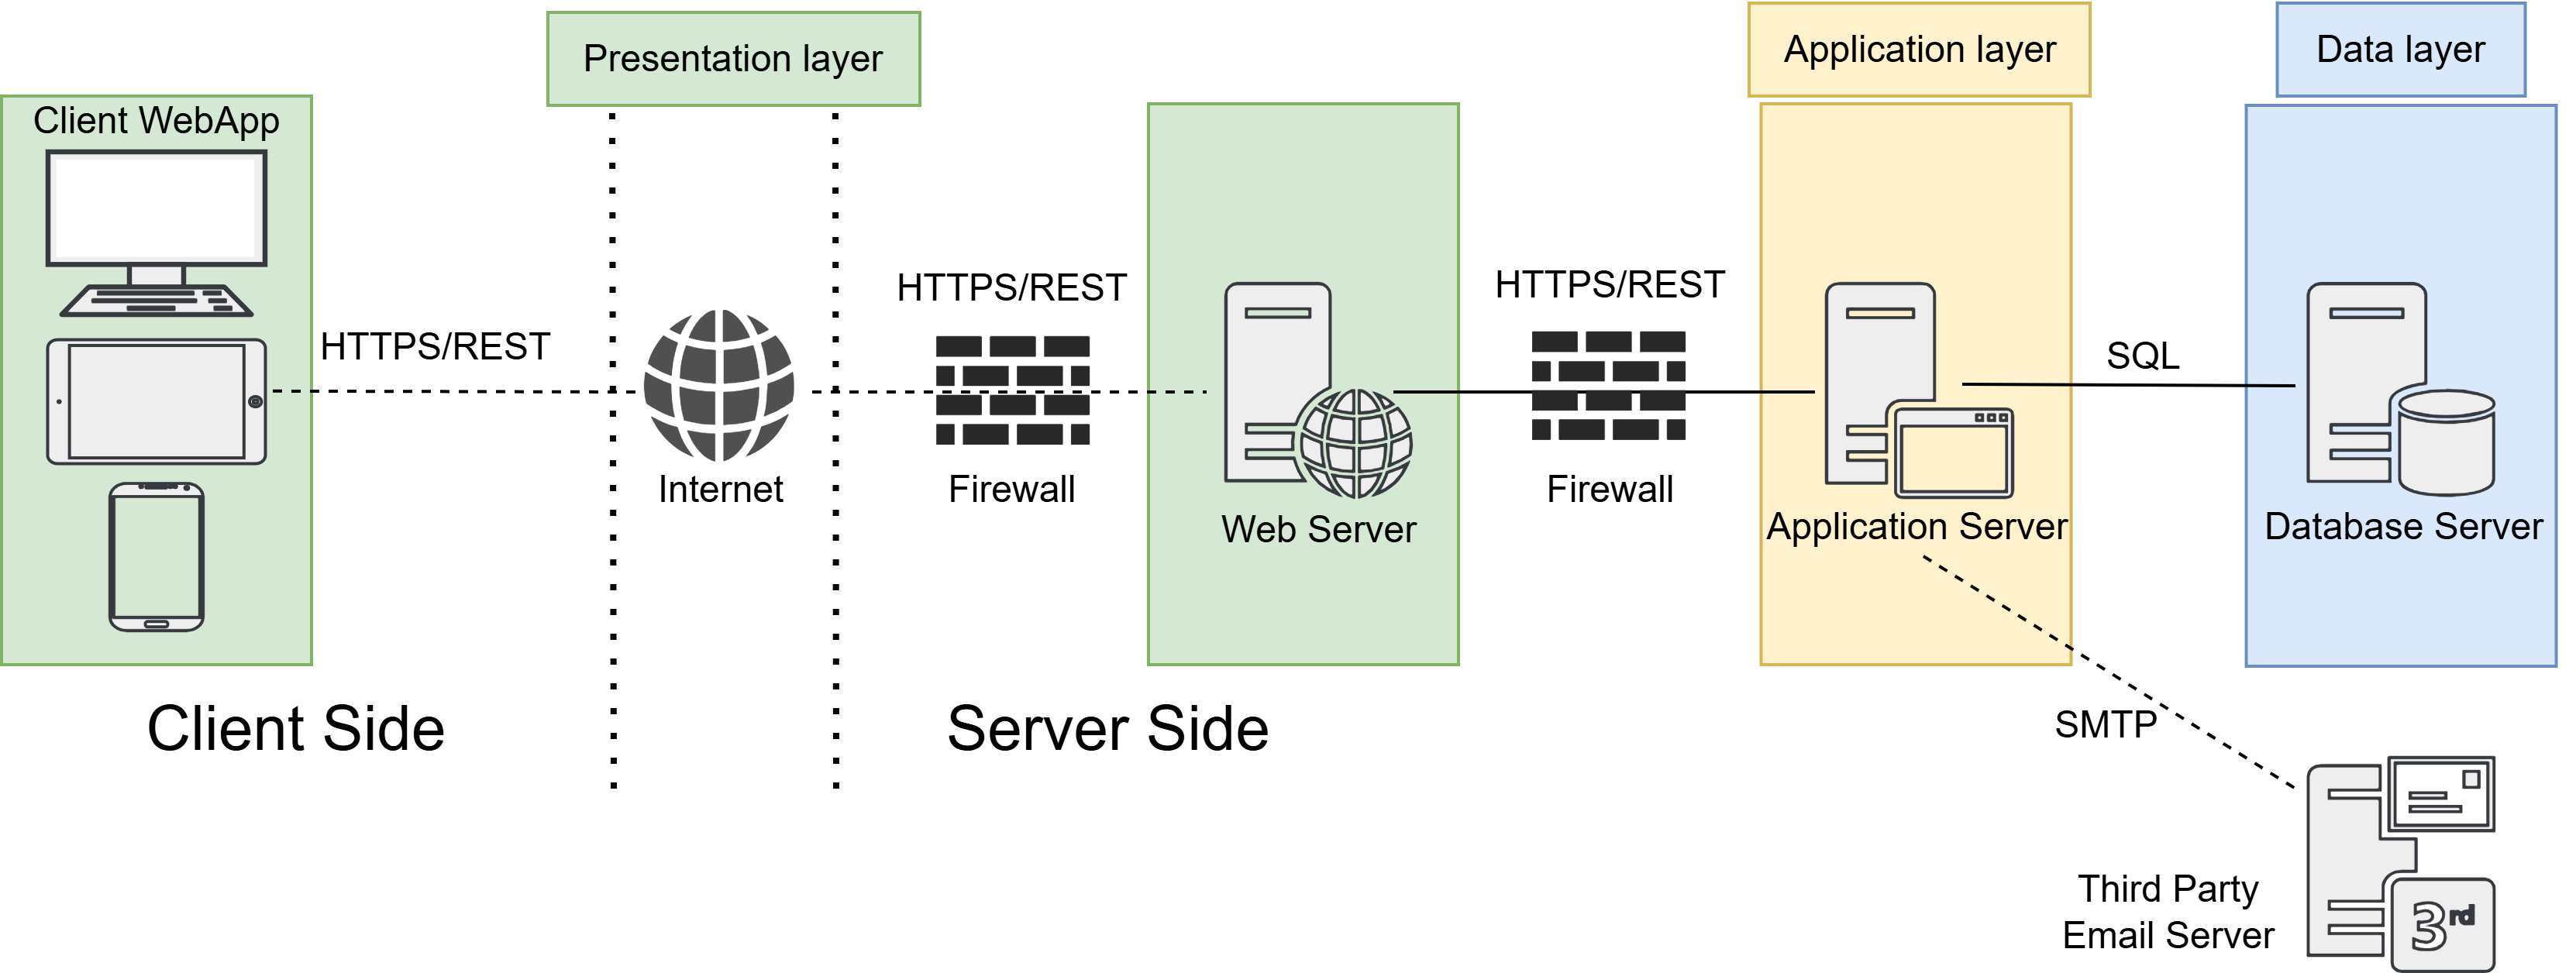
\includegraphics[width=1\textwidth]{Images/tiers_architecture.png}
    \caption{S\&C architectural overview}\label{fig:tiers_architecture}
\end{figure}

In the following paragraph we describe each tier presented in Figure \ref{fig:tiers_architecture}: and what layer it deploys:
\paragraph{Client Side}
\begin{itemize}
    \item \textbf{Web App:} It is the user interface. It will be responsible for managing the user interaction. This means that it will be responsible 
    for hosting part of the presentation layer. 
\end{itemize}

\paragraph{Server Side}
\begin{itemize}
    \item \textbf{Firewall:} It will be responsible for managing the security of the system, by filtering the incoming and outgoing traffic and restricting
    the access based on predefined rules. It will be placed between the Web Server and the Internet and between the Application Server and the Web Server.
    In this way, the web server will reside in a DMZ (Demilitarized Zone), while the application server will resides in a protected internal network.
    \item \textbf{Web Server:} It serves as a gateway between the client and the application server (backend). It will be responsible for hosting part 
    of the presentation layer. For example, it will be responsible for serving the web pages to the client, handling requests routing to the application
    server, managing load balancing, and handling security.
    \item \textbf{Application Server:} It will be responsible for managing the application logic. This means that it will host the application layer. For 
    example, it will be responsible for processing the client requests, execute the business logic, and coordinates with the database and email server.
    \item \textbf{Database Server:} It will be responsible for managing the data storage and the data access. This means that it will host the data layer.
    For example, it will be responsible for storing and retrieving the application data, and executing the database queries.
    \item \textbf{Mail Server:} It will be responsible for managing the email communication. This means that it will be responsible for sending emails to 
    the users. It is triggered by the application server.
\end{itemize}

The Figure\ref{fig:tiers_architecture} also shows how the tiers interact with each other. The Web App interacts with the Web Server through HTTPS/REST 
requests; the Web Server interacts with the Application Server through HTTPS/REST calls; the Application Server interacts with the Database Server through 
SQL queries; and the Application Server interacts with the Mail Server through SMTP requests.



\section{Components view}\label{sec:components view}
In this section we describe the components of the S\&C platform, their interactions, and the interfaces they expose. For understandability we divide the
components into two categories: high-level components and low-level components.

\subsection{High-level components and interactions}\label{subsec:high-level components and interactions}
\begin{figure}[H]
    \centering
    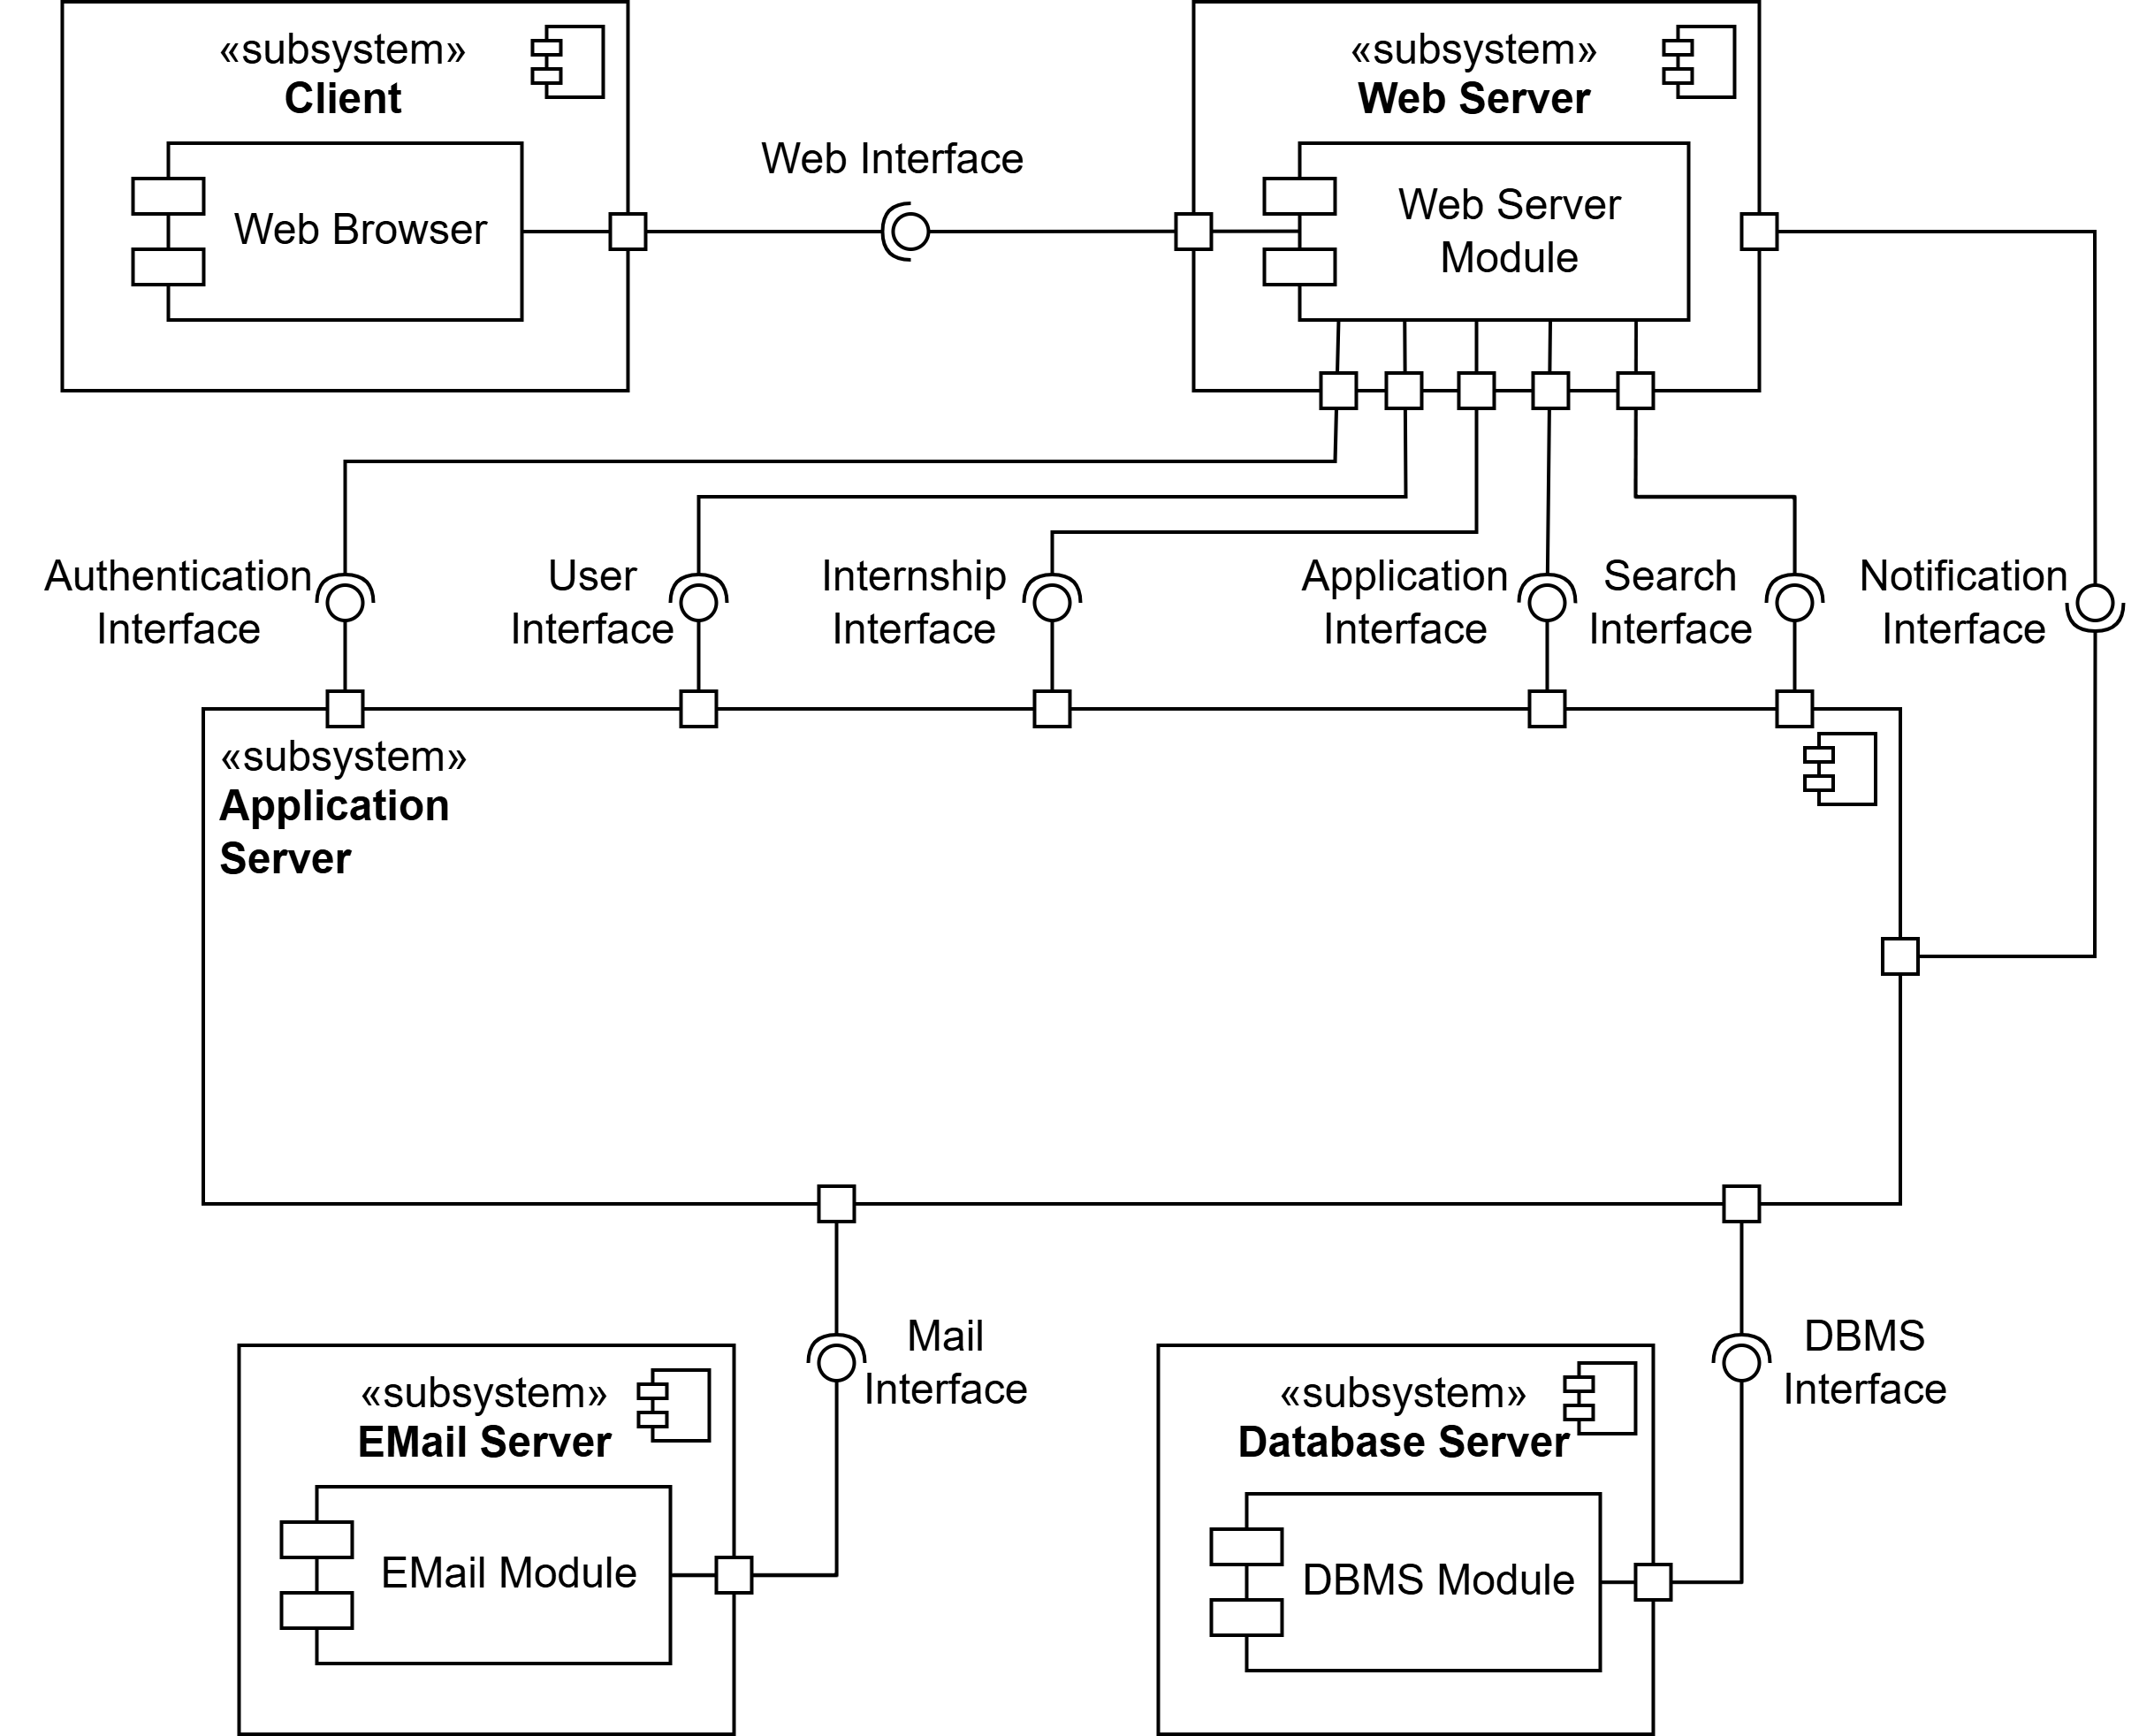
\includegraphics[width=1\textwidth]{Images/Components/HL_Component_Diagram.png}
    \caption{High Level Component Diagram}\label{fig:hl_component_diagram}
\end{figure}
In the figure above we show the high-level components of the S\&C platform. In particular we show which are the components that are run on each tier of 
the system.
\begin{itemize}
    \item \textbf{Web Browser:} It serves as the external interface for the user to interact with the platform. It sends requests to the Web Server and
    receives responses from it. It is responsible for rendering the web pages and handling user input.
    \item \textbf{Web Server Module:} It serves as a gateway between the client and the application server. It handles load balancing and security, 
    ensuring that requests are properly routed through the interfaces that are provided by the application server. It also provides the Notification 
    Interface, which allows the Web Server Module to send notifications to users.
    \item \textbf{Application Server:} Hosts all the system's internal components and provides the following interfaces: Authentication Interface, User 
    Interface, Internship Interface, Application Interface, and Search Interface. 
    \item \textbf{DBMS:} It communicates with the application server through the DBMS Interface and is responsible for managing the data storage and 
    retrieval operations. It ensures data consistency and integrity, and provides mechanisms for data backup and recovery. 
    \item \textbf{Email Server:} It is responsible for the sending of emails for user registration confirmation. The Application Server interacts with 
    the Email Server via the Email Interface to send these emails.
\end{itemize}

\subsection{Low-level components and interactions}\label{subsec:low-level components and interactions}
\begin{figure}[H]
    \centering
    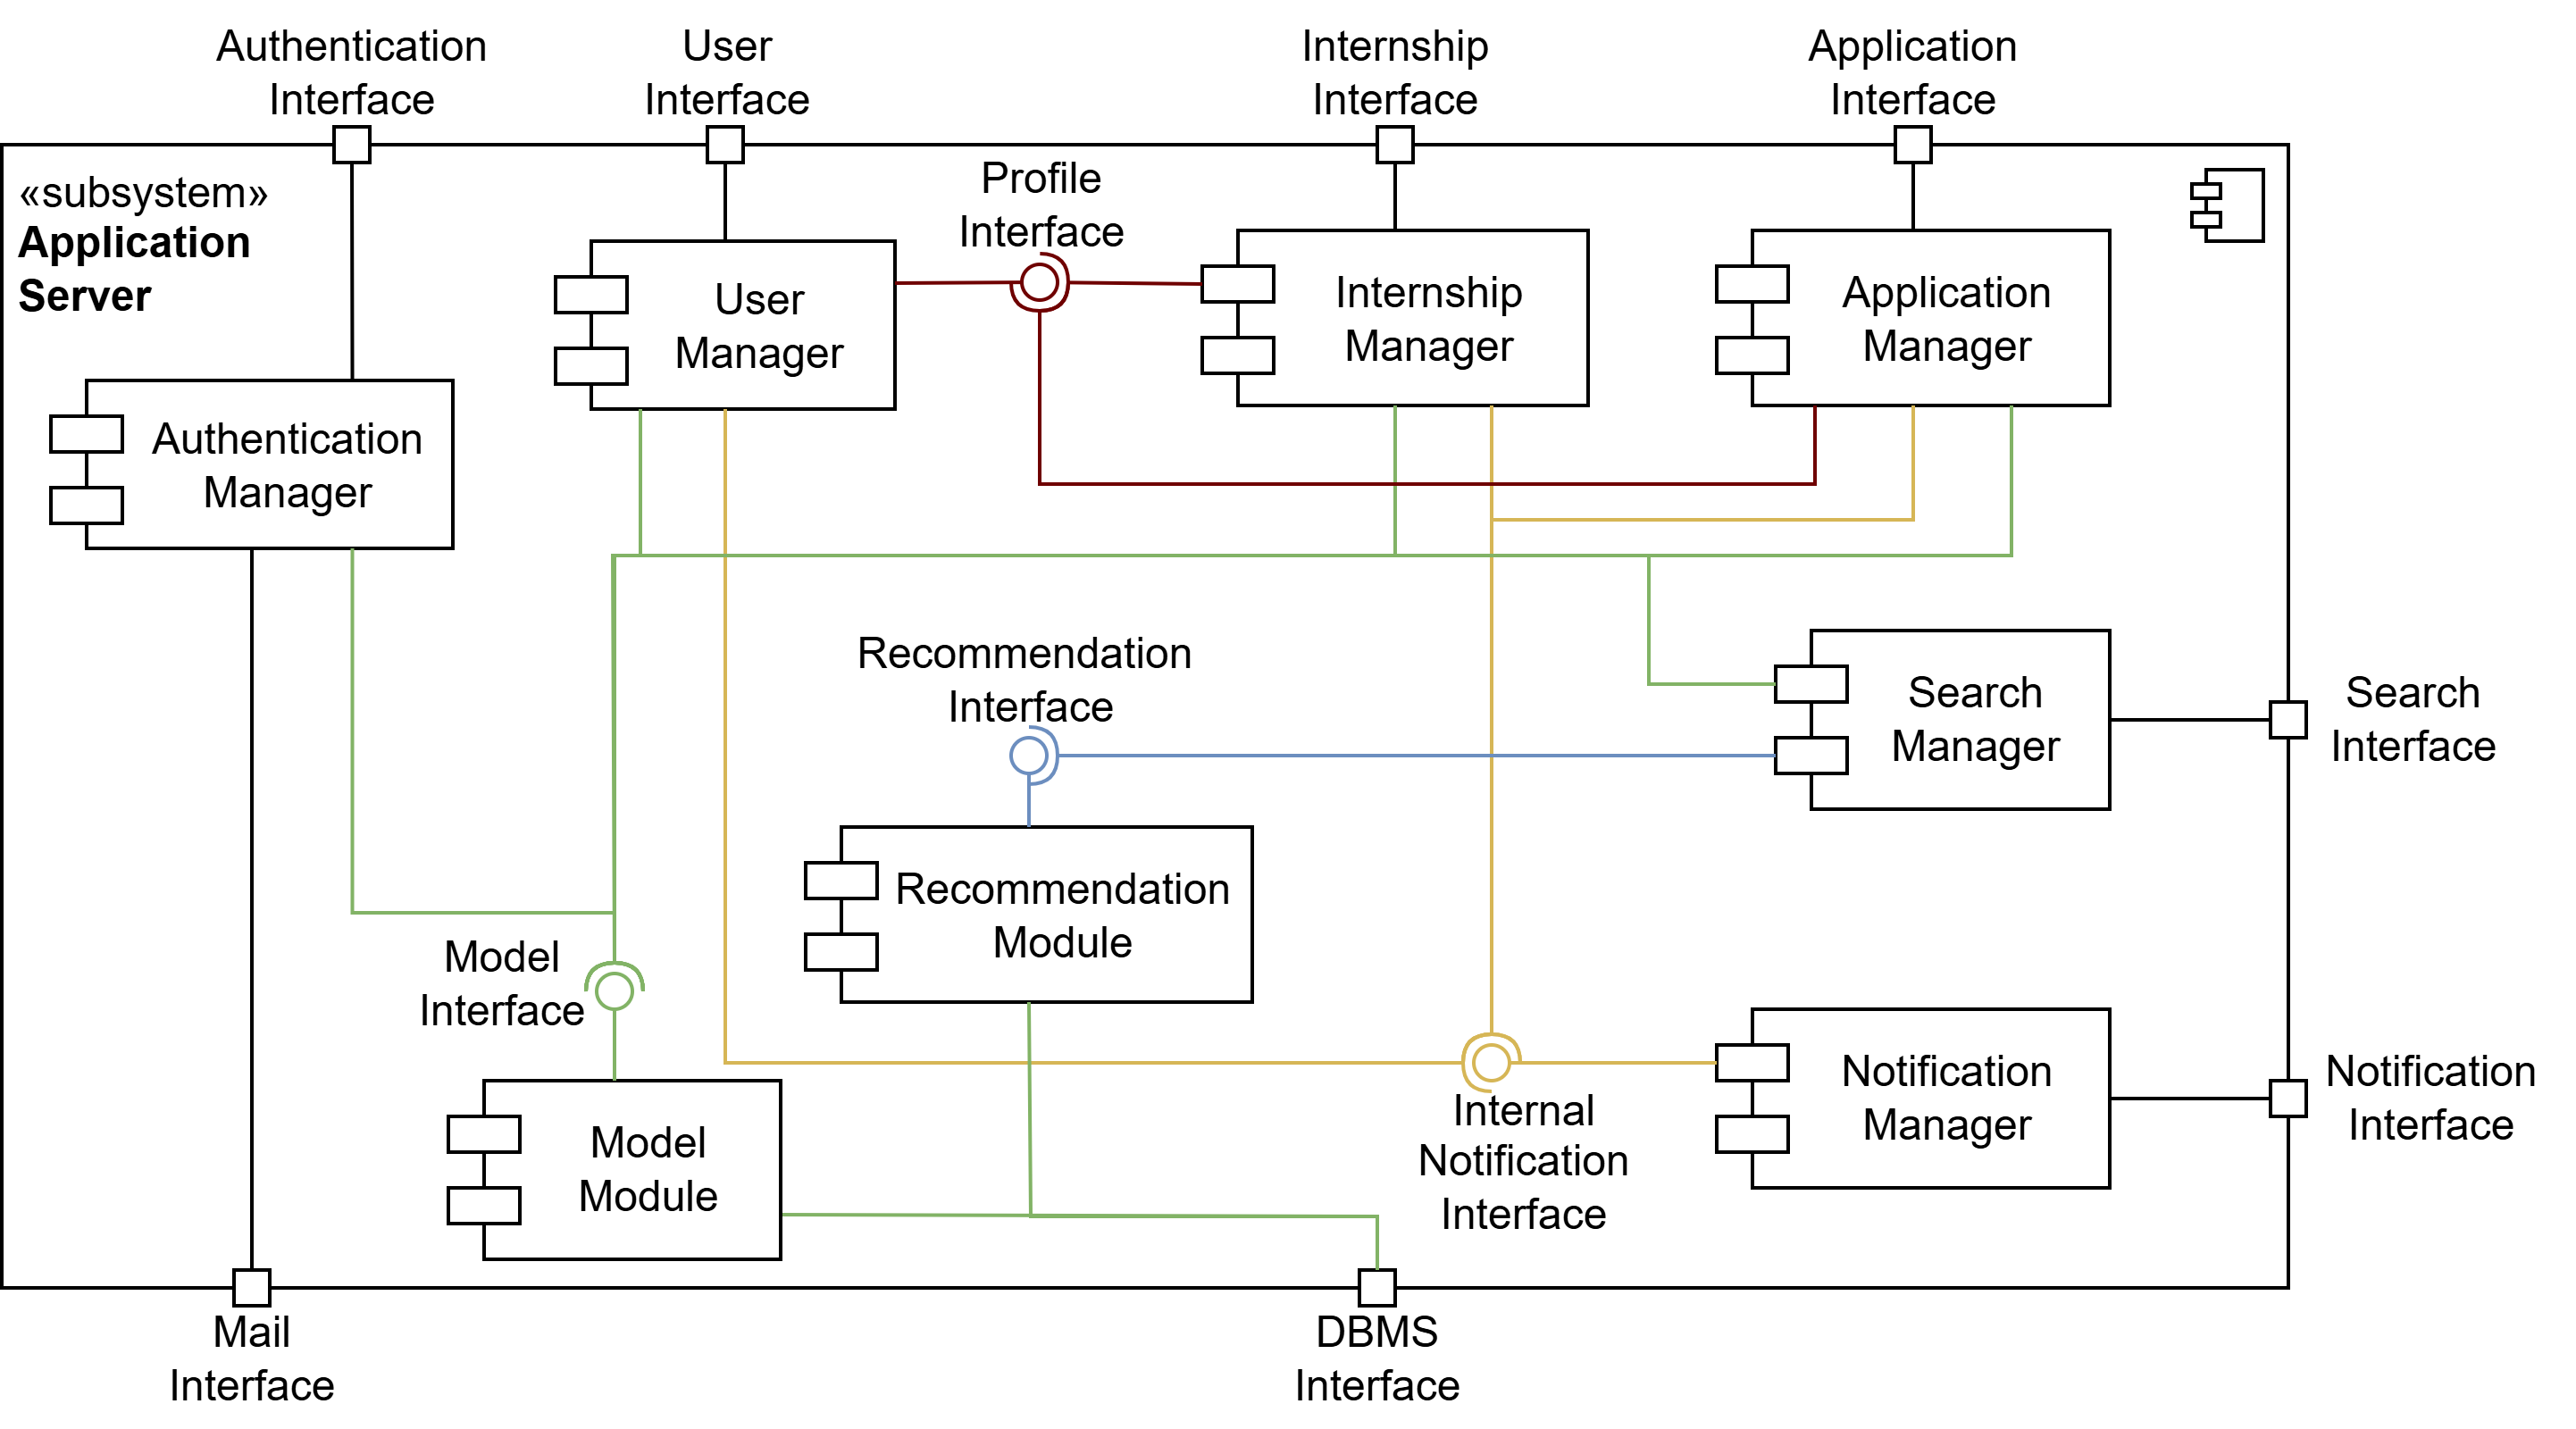
\includegraphics[width=1\textwidth]{Images/Components/LL_Component_Diagram.png}
    \caption{Low Level Component Diagram}\label{fig:ll_component_diagram}
\end{figure}
In Figure \ref{fig:ll_component_diagram}, we show the low-level components of the platform. In particular, these components provide more detailed 
insights into the internal workings of the Application Server. The low-level components are divided as follows:
\subsubsection{Authentication Manager}
This component manages user authentication and authorization processes. It interacts with the Model Module through the provided
interface in order to store and retrieve information from the database. It includes the following subcomponents:
\begin{itemize}
    \item \textbf{Registration Manager:} It is responsible for managing the user registration process, including the creation of new user accounts 
    and sending verification emails through the Mail Interface.
    \item \textbf{Login Manager:} It is responsible for managing the user login process, including verifying user credentials and maintaining user sessions.
\end{itemize}
\begin{figure}[H]
    \centering
    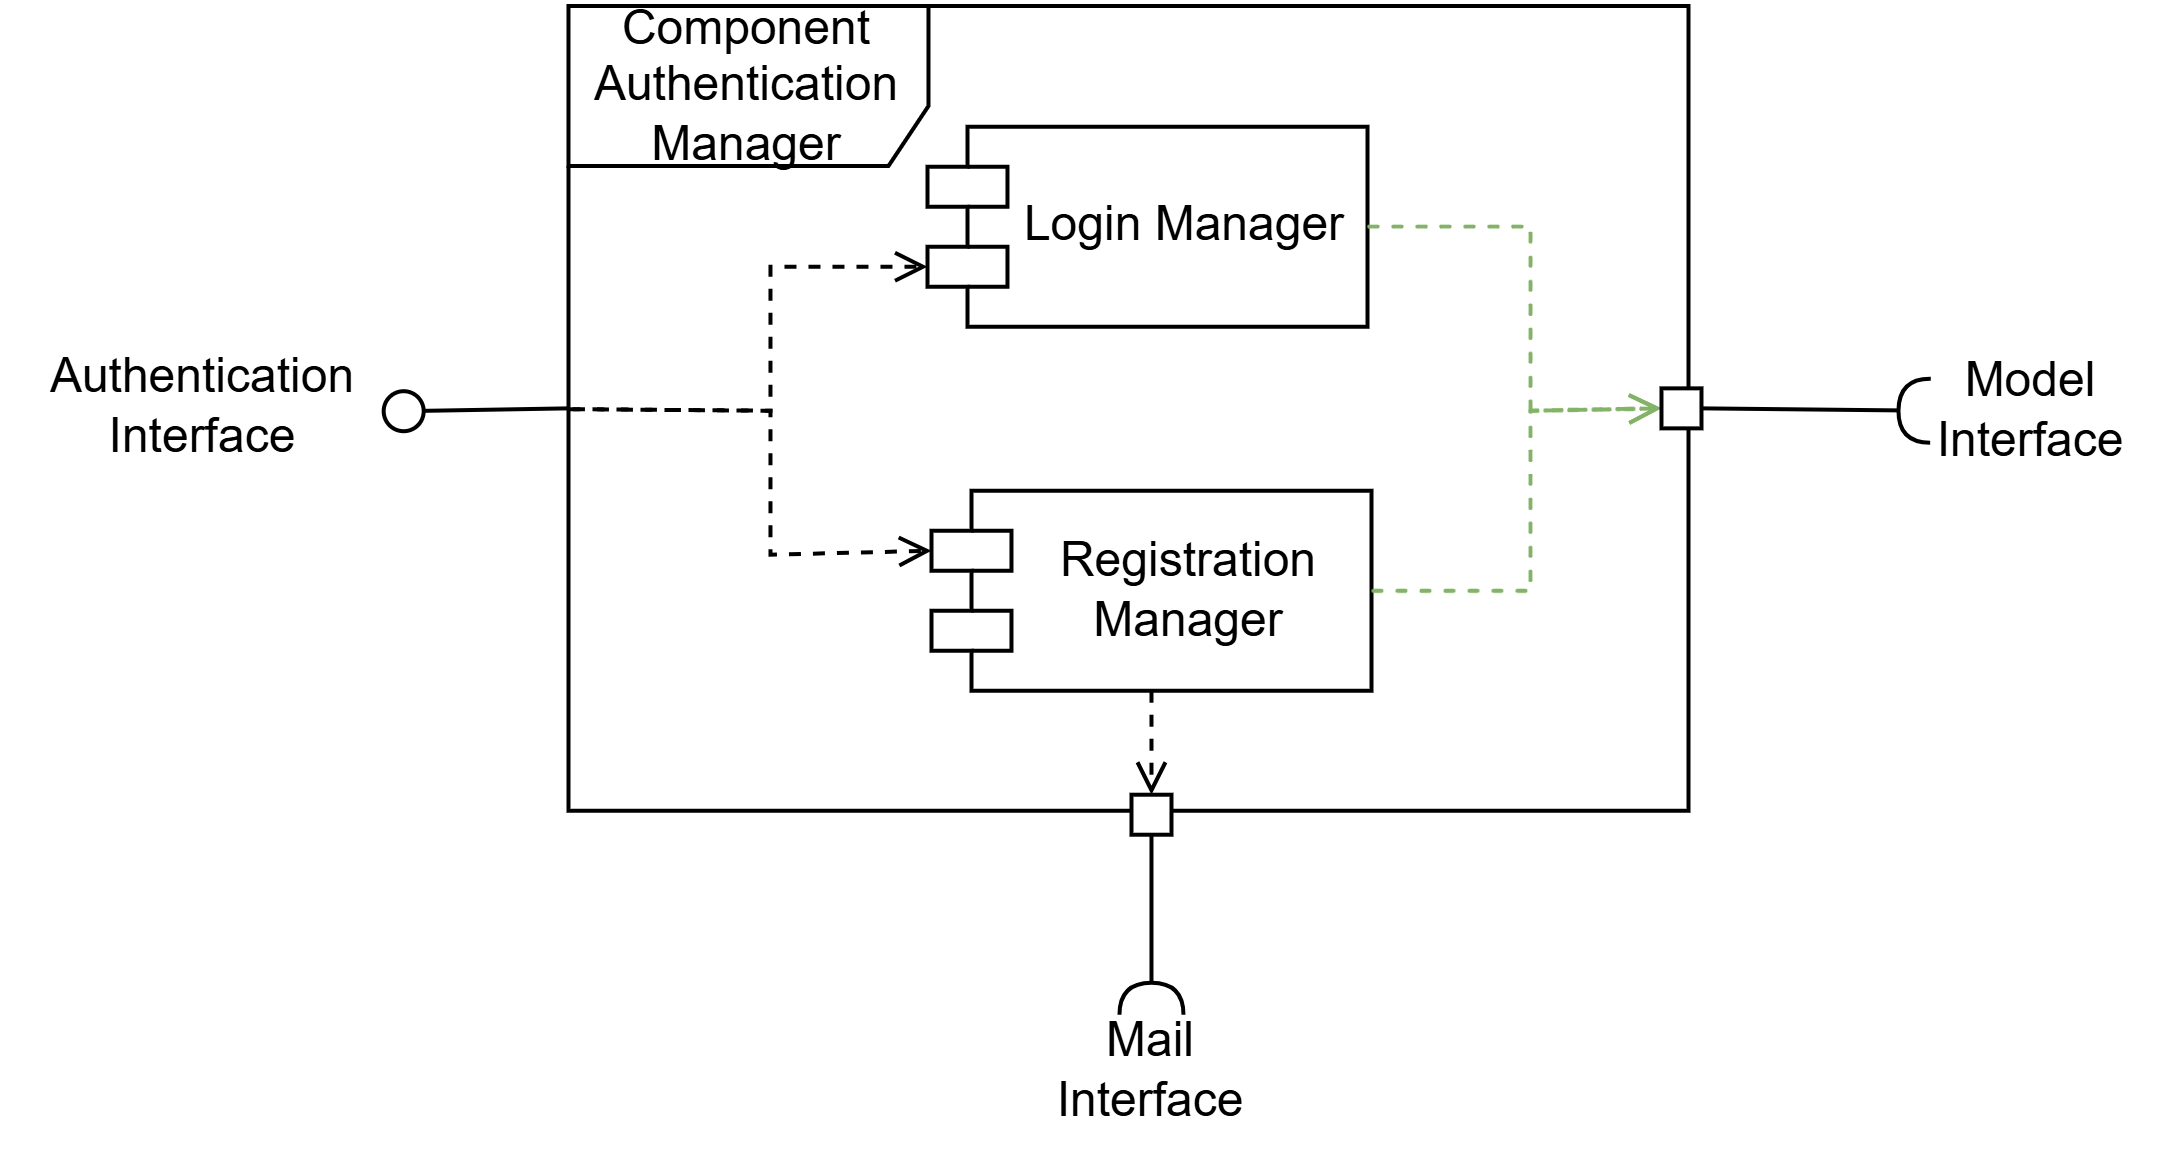
\includegraphics[width=0.75\textwidth]{Images/Components/auth_Component.png}
    \caption{Authentication Manager}\label{fig:auth_manager}
\end{figure}
\subsubsection{User Manager}
This component is responsible for managing user-related operations, such as user profile management and visualization, and handling user-specific 
notifications. It interacts with the Model Module to store and retrieve user information from the database.
\begin{itemize}
    \item \textbf{View Profile Manager:} Provides users with an overview of their activities and notifications. It provides a Profile Interface that
    allows other components to access user data.
    \item \textbf{Profile Modification Manager:} Allows users to view and edit their personal information.
\end{itemize}
\begin{figure}[H]
    \centering
    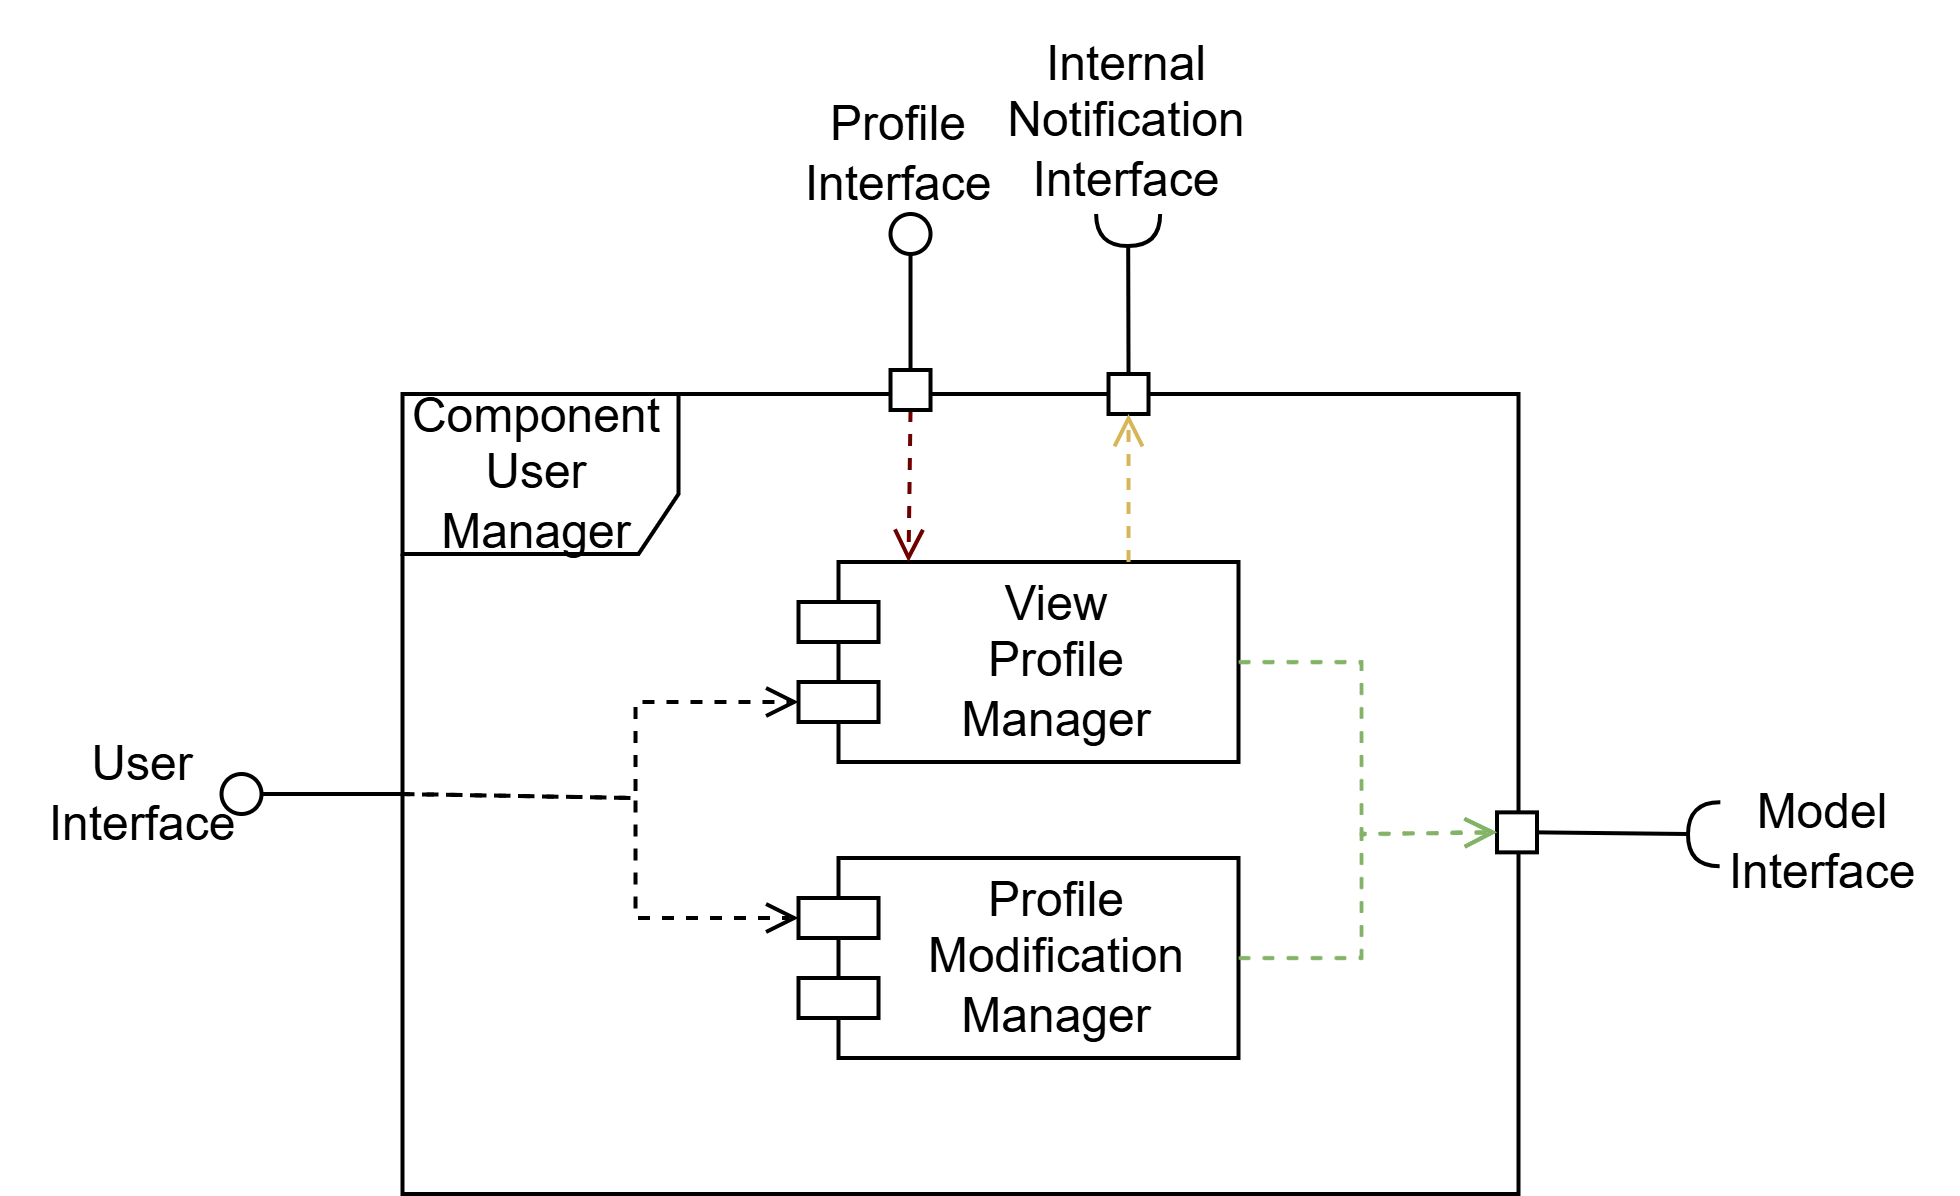
\includegraphics[width=0.75\textwidth]{Images/Components/user_Component.png}
    \caption{User Manager}\label{fig:user_manager}
\end{figure}
\subsubsection{Internship Manager}
The Internship Manager is the component used by the S\&C platform to manage internship-related operations. It interacts with the Model Module to store
and retrieve internship information and related data (such as chat messages and feedback) from the database. It includes the following subcomponents:
\begin{itemize}
    \item \textbf{Creation Manager:} Manages the creation of internship and their posting. 
    \item \textbf{View Internship Information Manager:} Manages the display of internship information when users request them.
    \item \textbf{Selection Manager:} Manages the selection process for internships. It allows companies to go through the list of applications and select 
    candidates for their internships. After the interview phase, it also allows them to decide whether to accept or reject a candidate for the internship. 
    It interacts with the Internal Notification Interface to notify students in case they are selected for interviews and in case they are accepted or rejected 
    for an internship.
    \item \textbf{Chat Manager:} Manages the chat functionality between student and company. It interacts with the Notification Manager through the provided
    interface to notify users when they receive a new message.
    \item \textbf{Feedback Manager:} Manages the feedback system for internships, allowing both companies and students to provide feedback on their internship 
    experience. It interacts with the Notification Manager through the provided interface to notify users when they receive new feedback.
\end{itemize}
The View Internship Information Manager, Chat Manager, and Feedback Manager also interact with the View Profile Manager through the provided Profile Interface,
since they need to show to both students and companies other users profile information.
\begin{figure}[H]
    \centering
    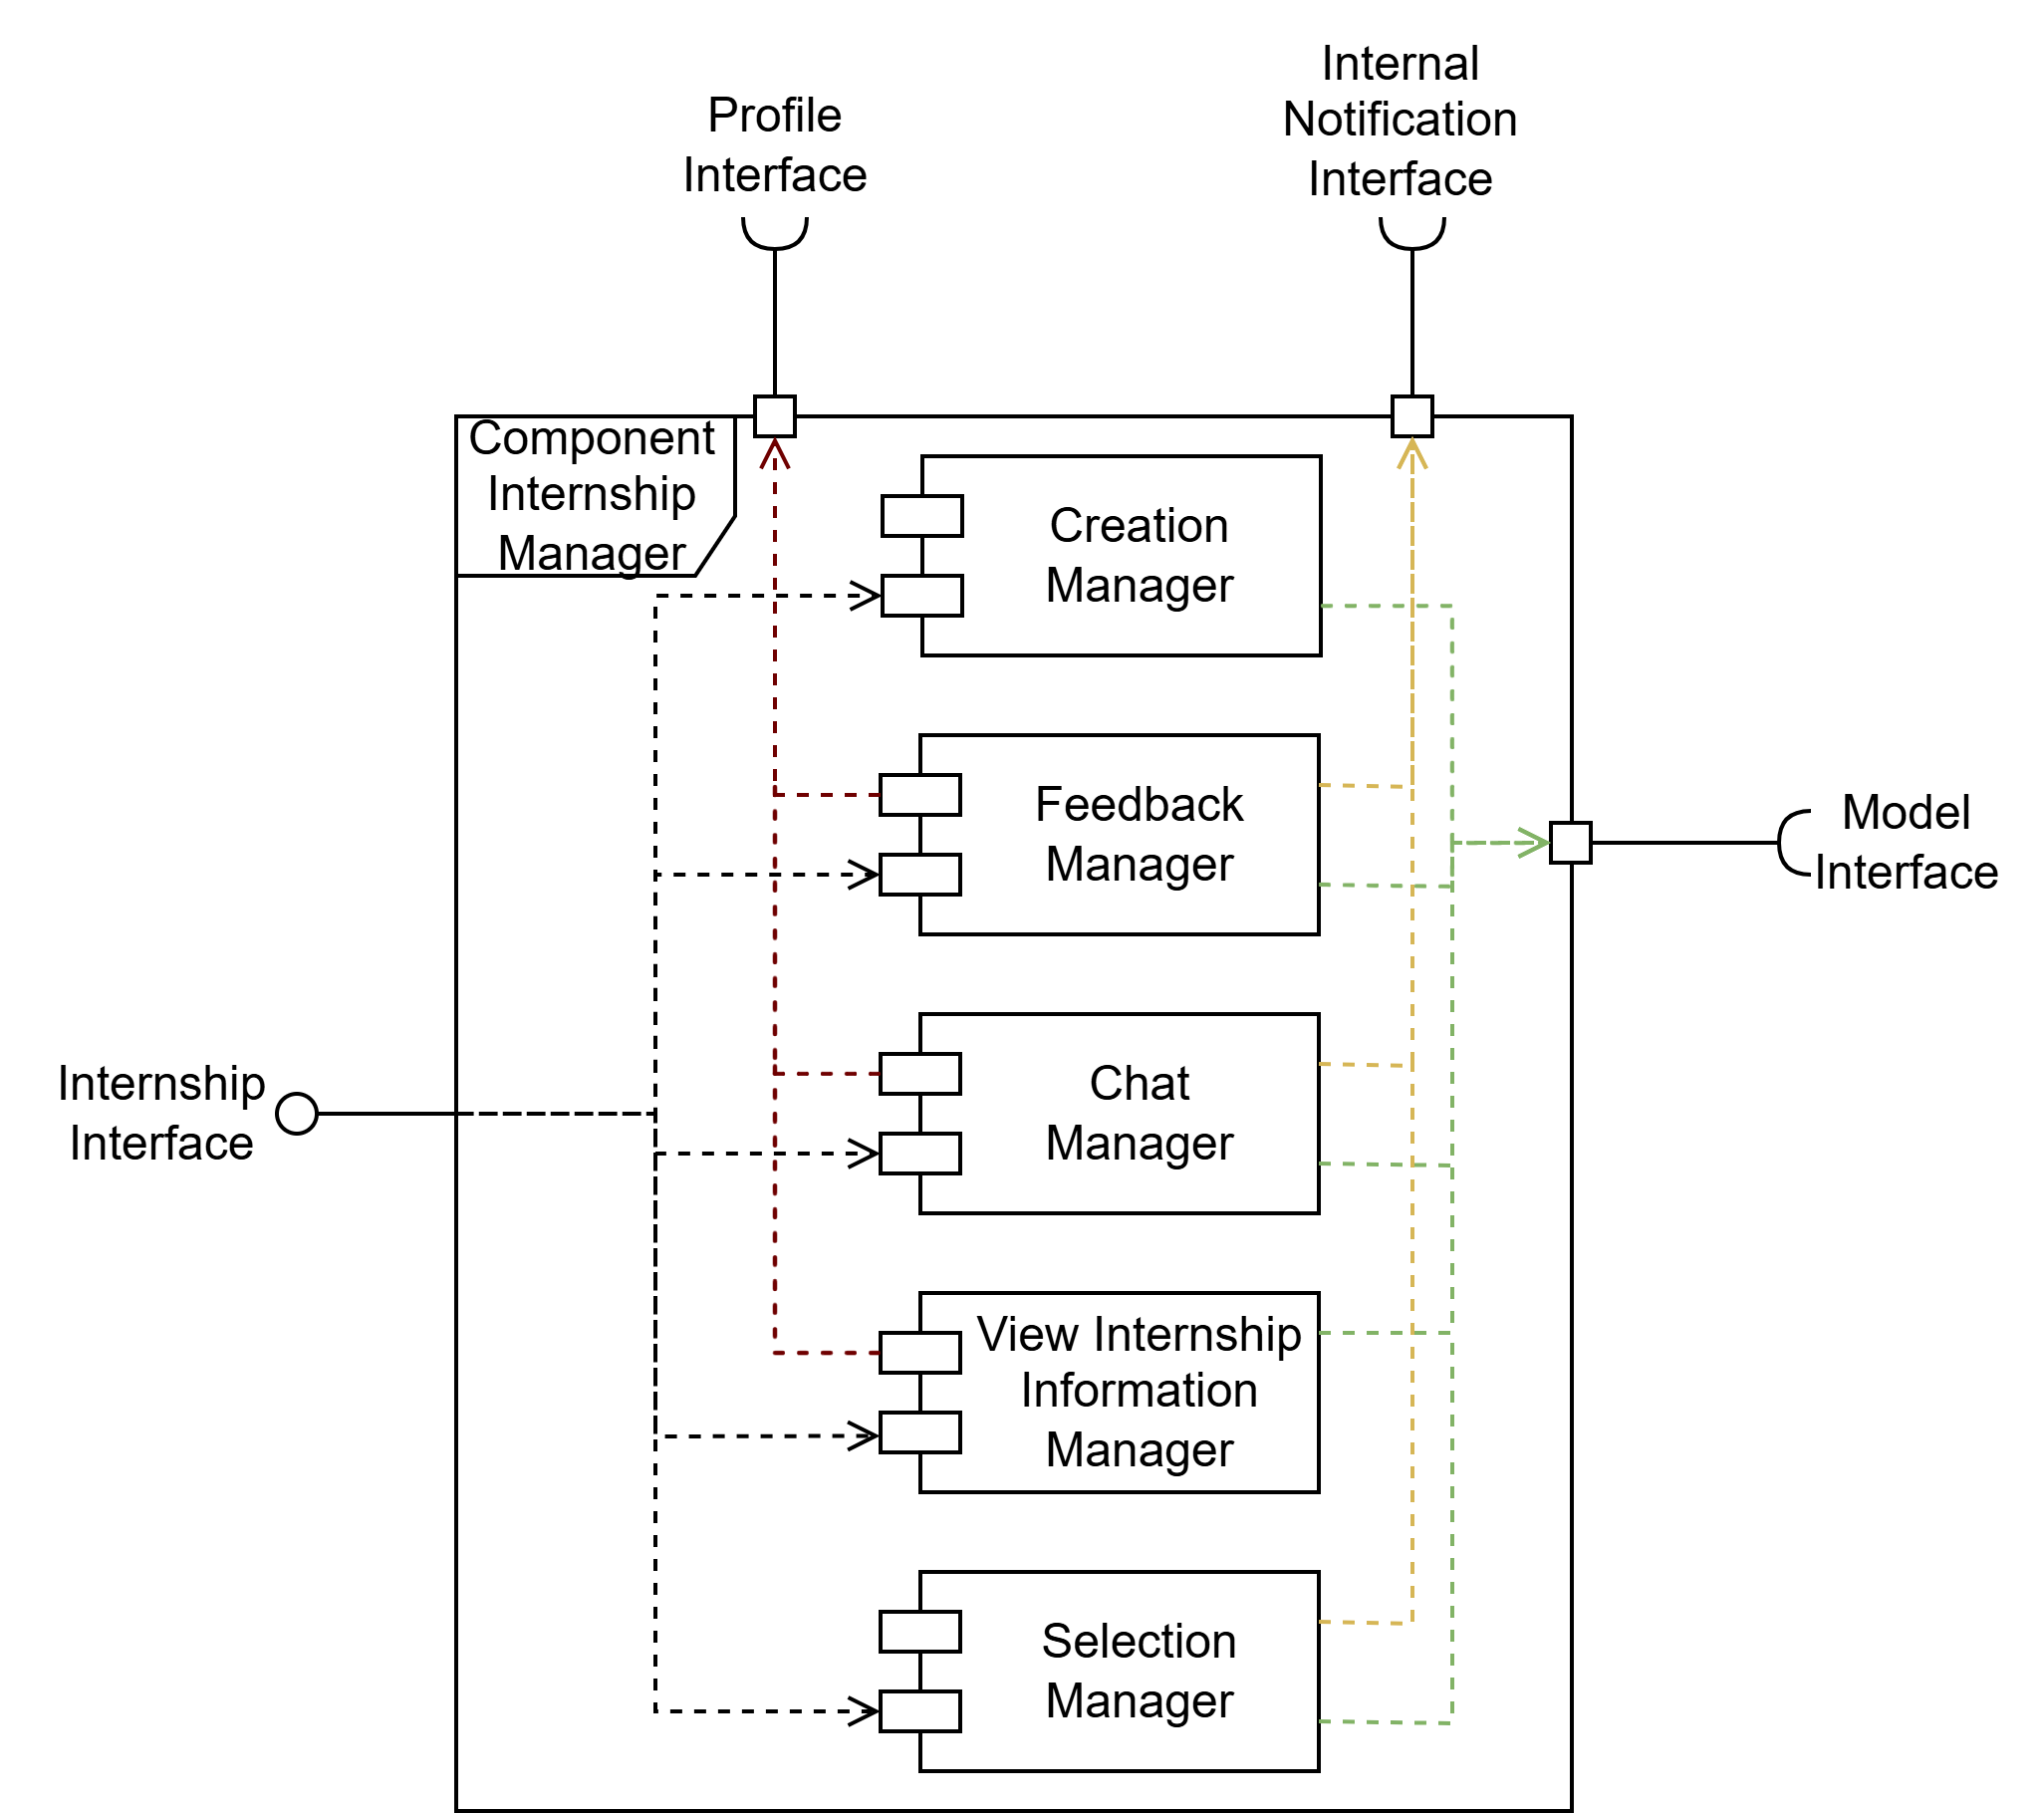
\includegraphics[width=0.75\textwidth]{Images/Components/internship_Component.png}
    \caption{Internship Manager}\label{fig:internship_manager}
\end{figure}
\subsubsection{Application Manager}
The Application Manager is the component used by the S\&C platform to handle every aspect of the application process for internships. It interacts with the
Model Module to store and retrieve application information and related data from the database. It includes the following subcomponents:
\begin{itemize}
    \item \textbf{Submission Manager:} Handles the submission of applications for internships. It allows students to apply for internships and submit their
    applications. It also allows candidates who have been accepted for the internship to accept or reject the offer from the company. It interacts with the 
    Internal Notification Interface to notify students when their application status changes.
    \item \textbf{View Application Information Manager:} Manages the display of application information to users who request them and have the rights to access
    them.
    \item \textbf{Interview Manager:} Manages the interview process for applications; it allows companies to create and modify interview forms and record 
    the results of interviews. It interacts with the Internal Notification Interface to notify students when they are selected for interviews, and notify 
    companies when the results of the interviews are available. 
    \item \textbf{Questionnaire Manager:} Manages the questionnaire system for applications, allowing students to respond to interview questions and both 
    students and companies to view the responses. It interacts with the Internal Notification Interface to notify companies when a student has completed the 
    interview form.
\end{itemize}
The View Application Information Manager, Interview Manager, and Submission Manager also interact with the View Profile Manager through the provided Profile
Interface, since they need to show to both students and companies other users profile information.
\begin{figure}[H]
    \centering
    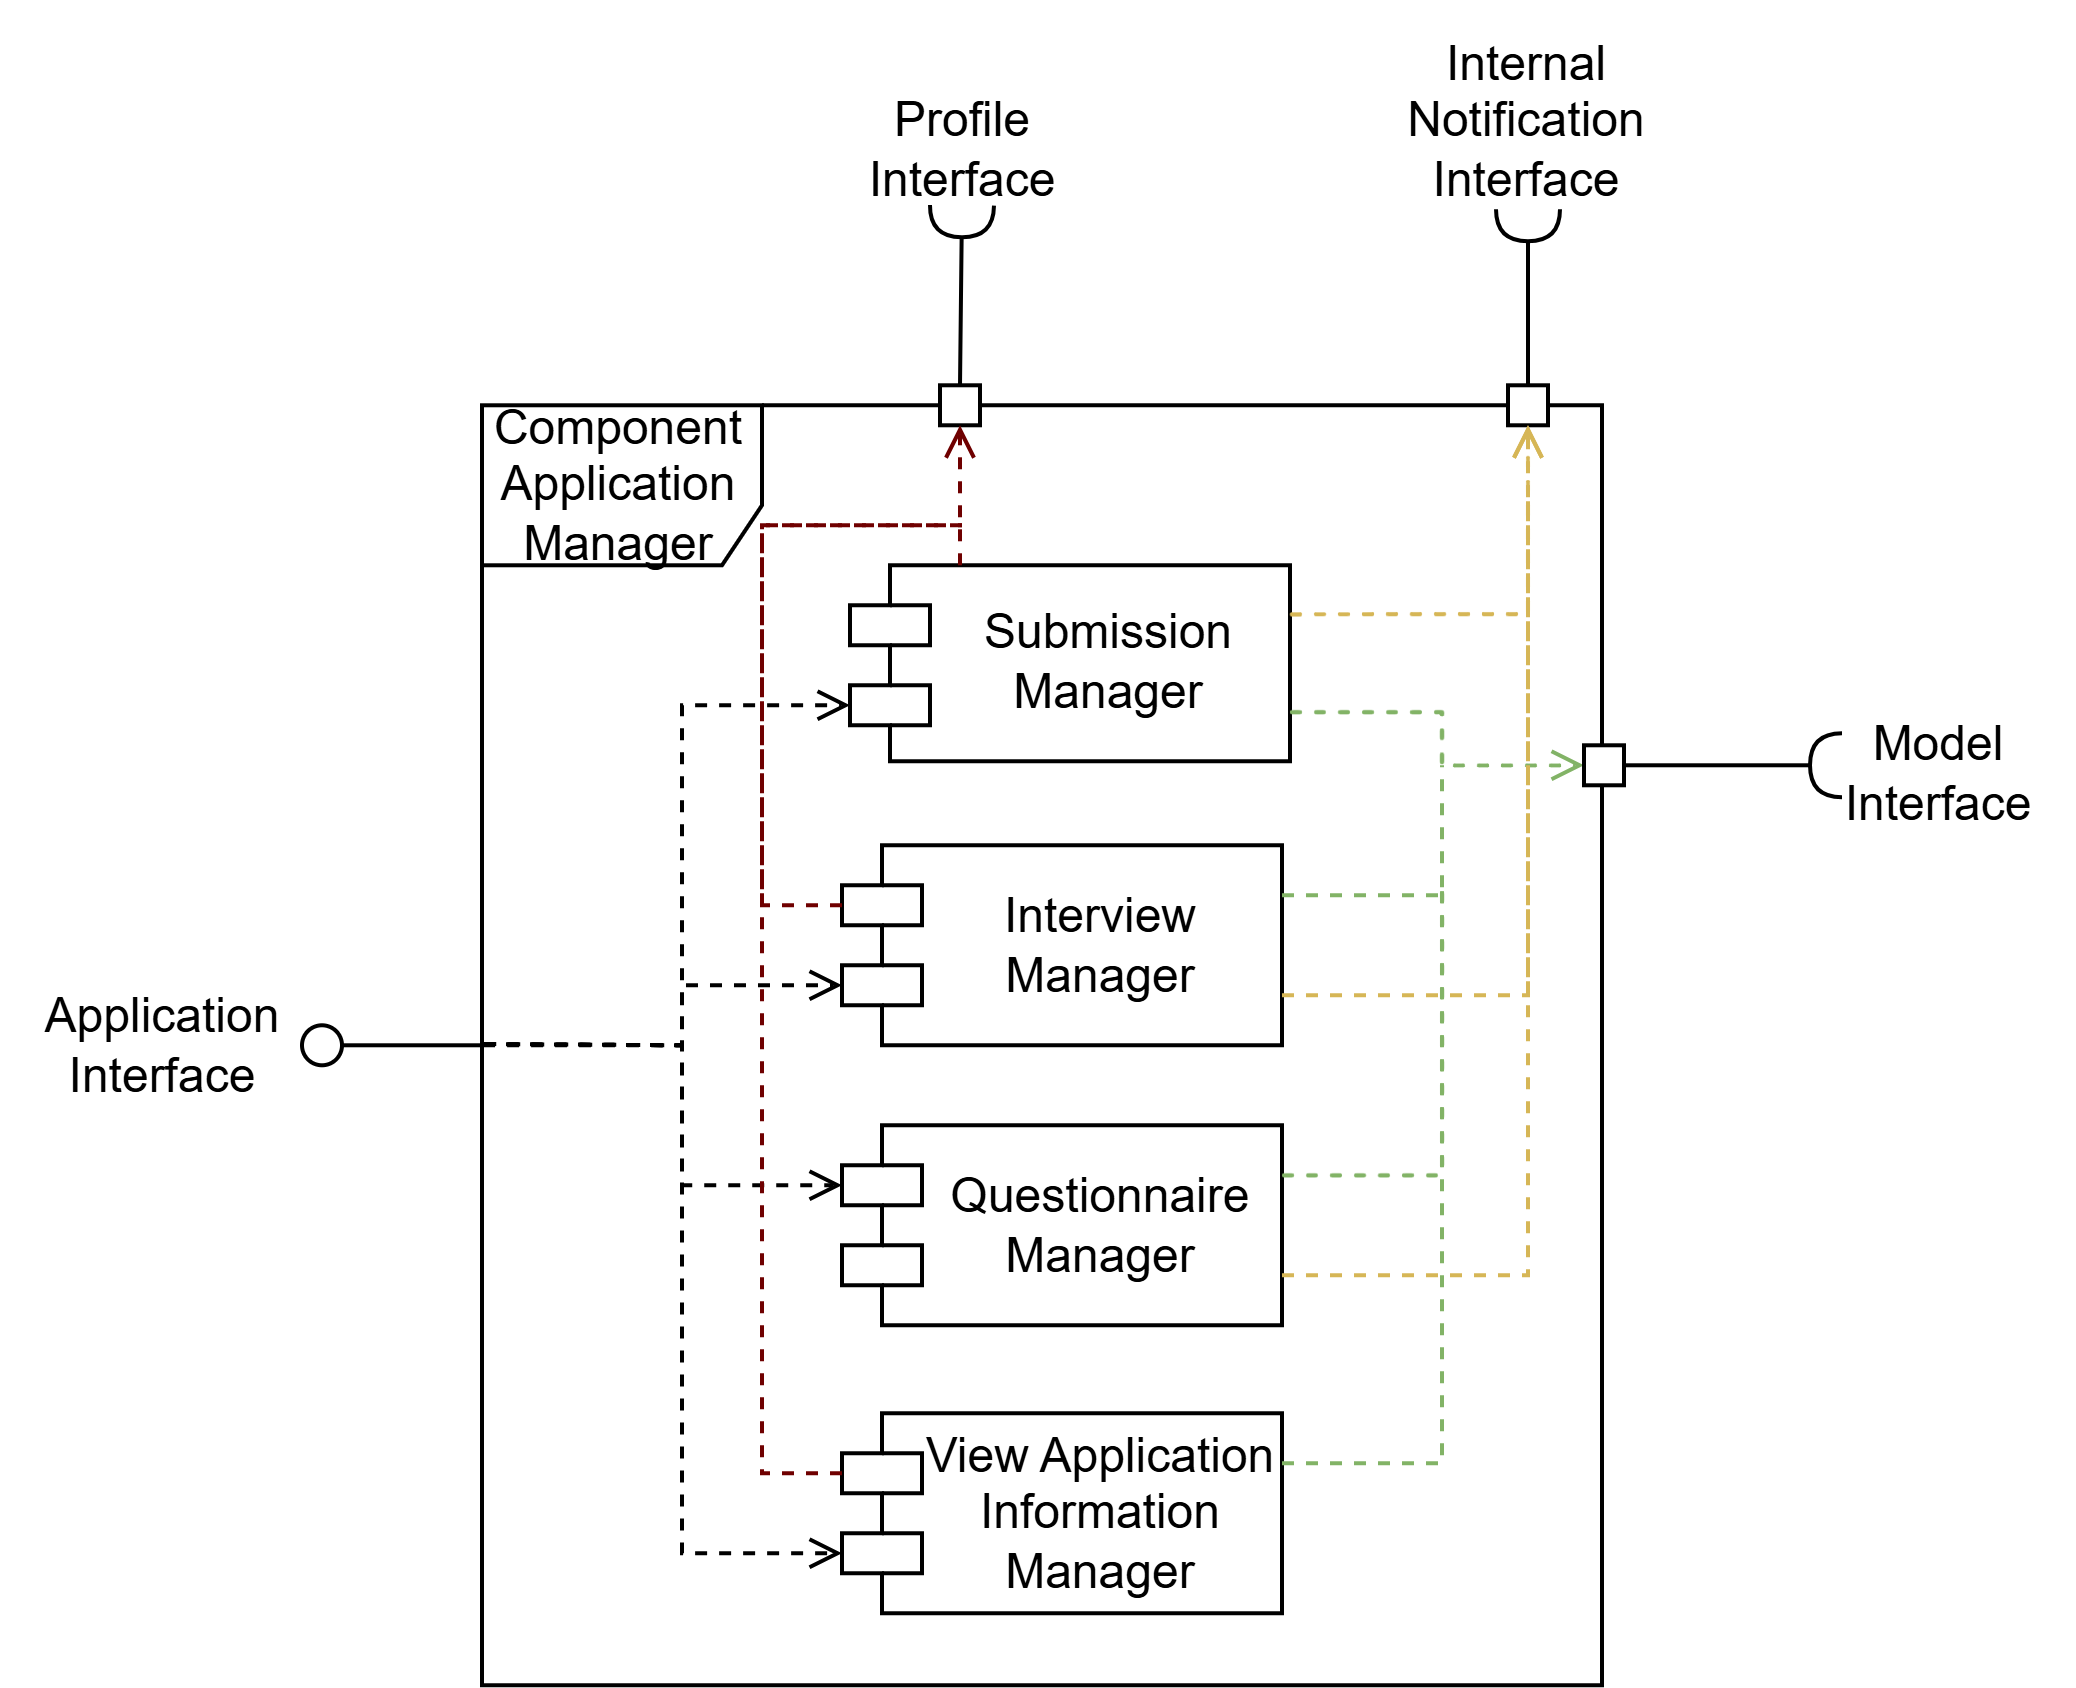
\includegraphics[width=0.75\textwidth]{Images/Components/application_Component.png}
    \caption{Application Manager}\label{fig:application_manager}
\end{figure}
\subsubsection{Search Manager}
The Search Manager is responsible for managing the search functionality of the platform, allowing users to search using filters or keywords. It interacts with 
the Model Module to retrieve search results from the database. It also interacts with the Recommendation Module to provide personalized, real-time 
recommendations to users.
\subsubsection{Notification Manager}
The Notification Manager is responsible for managing the notification system of the platform, allowing users to receive real-time updates on their activities.
It provides an Internal Notification Interface that allows other components to send notifications to users.
\subsubsection{Recommentation Module}
The Recommendation Module is responsible for generating personalized recommendations for users based on their interests, skills, and activities. It interacts
directly with the DBMS Server to retrieve the necessary information from the database in order to provide recommendations to users. It also interacts with the 
Search Manager to provide real-time recommendations based on search results.
\subsubsection{Model Module}
The Model Module is responsible for managing the data storage and retrieval operations of the platform. It interacts with the DBMS to store and retrieve
information from the database. It provides the Module Interface that allows other components to access the data stored in the database.



\section{Deployment view}\label{sec:deployment view}
\begin{figure}[H]
    \centering
    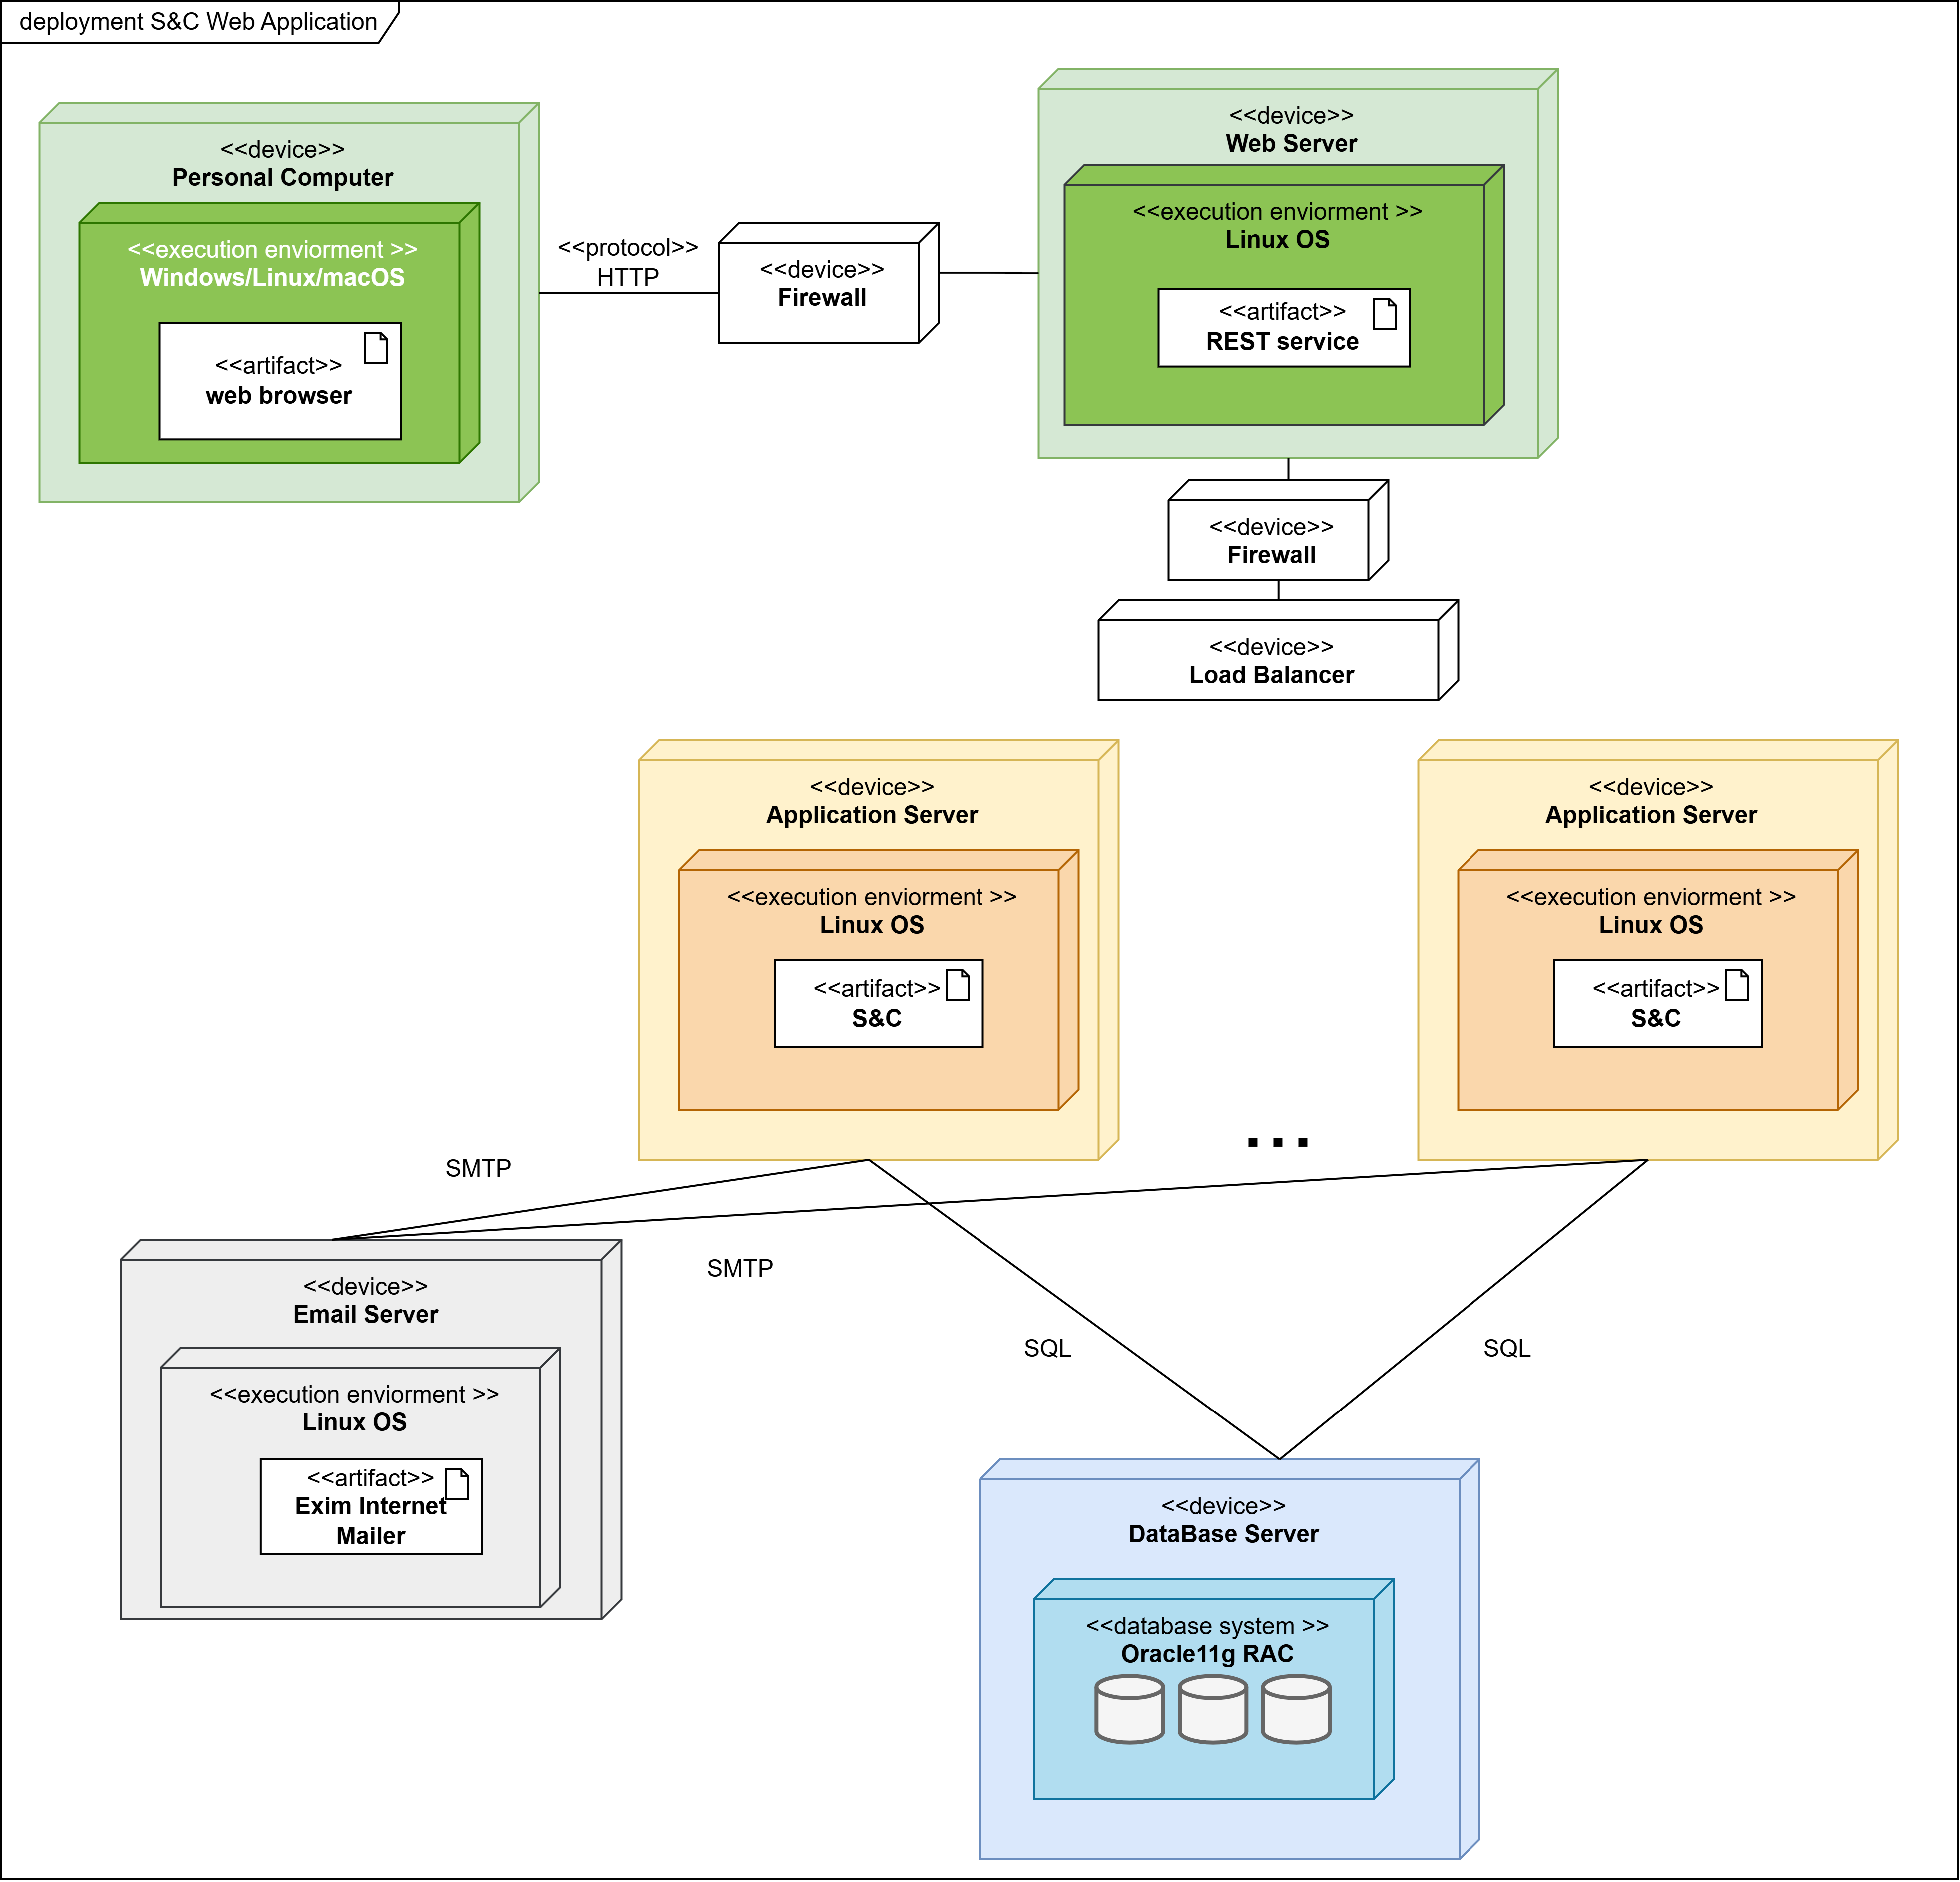
\includegraphics[width=1\textwidth]{Images/Deployment_View.png}
    \caption{S\&C deployment diagram}\label{fig:deployment_diagram}
\end{figure}
The infrastructure of the S\&C platform is described in below using a deployment diagram and a description of the components and their interactions.
As described at the beginning of this document, the system is divided into three tiers: the presentation layer, the application layer, and the data layer.
The deployment diagram in Figure \ref{fig:deployment_diagram} shows the physical distribution of the components across different servers and the communication
between them.

\begin{itemize}
    \item \textbf{Personal Computer:} Anyone interested in using the platform can access it through any type of personal computer. Users can also access the 
    platform using any device capable of running a web browser. This component communicates and interacts with the Web Server via HTTPS protocols and RESTful 
    API services.
    \item \textbf{Web Server:} The Web Server hosts the web application and serves web pages to users. It handles HTTP requests from clients and forwards them 
    to the Application Server. Together with the Firewall and Load Balancer, it ensures the security, scalability, and availability of the system. It acts as 
    a gateway between the client and the Application Server.
    \item \textbf{Application Server:} This component contains the core application logic of the platform, managing the operations necessary to provide services 
    and functionalities to users. Thanks to RESTful API services and the Load Balancer, it can handle multiple requests simultaneously without the risk of 
    overloading or crashing. It interacts with the Database Server to access or store data, such as recording a student's new internship. Additionally, it 
    communicates with the Mail Server, particularly during user registration, to authenticate email addresses and verify user identities.
    \item \textbf{Database Server:} Most primary operations of the platform require frequent interaction with the Database Server. This component manages 
    personal data, tracks the progress of applications and internships, stores chat histories between users, and more. The Application Server retrieves or 
    stores data using SQL queries.
    \item \textbf{Mail Server:} During the registration process, the platform requires users to verify their email addresses to confirm their identity and 
    complete account creation. The Application Server interacts with the Mail Server via SMTP requests to send verification emails.
    \item \textbf{Firewall:} The Firewall protects the core components of the system by filtering incoming and outgoing traffic and restricting access based on 
    predefined rules. For example, if an unauthorized individual attempts to access the Application Server and modify data in the Database Server without proper 
    credentials, the Firewall blocks the attempt, preventing unauthorized access.
    \item \textbf{Load Balancer:} The Load Balancer distributes incoming client requests to ensure that no one application server is overwhelmed to operate at 
    peak efficiency. It is placed between the Web Server and the Application Server, in order to optimize the performance and availability of the system.
\end{itemize}

\section{Component interfaces}\label{sec:component interfaces}
In the following paragraphs, we describe the interfaces of the main components of the platform specifying the methods that each component can perform.
Note: 

- \textit{userId} are unique identifiers generated by the system for each user once they register on the platform and are used to access the data related to 
that user.

- \textit{userTypes} enumeration is used to distinguish between the different types of users that can register on the platform: Student, Company, University.

- \textit{SearchType} enumeration used to distinguish between the different types of searches that can be performed on the platform: Internship and User Profile.

- \textit{NotificationType} enumeration used to distinguish between the different types of notifications that can be sent on the platform in order to handle 
them in a different way.

- \textit{InternshipID} is a unique identifier generated by the system for each internship published successfully and is used to access the data related to 
that internship.

- \textit{ChatID} is a unique identifier generated by the system for each chat created between two users and is helpful to access the data related to that 
chat more easily.

- \textit{ApplicationID} is a unique identifier generated by the system for each application submitted by a student for an internship and is used to access 
the data related to that application and take a track of its status.
\paragraph{Registration Manager}
\begin{itemize}
    \item[-] registration (String email, String password, String name, String surname, University university, List[Field] interests, List[String] skills): Boolean
    \item[-] registration (String email, String password, String legalName, String EIN, String department, List[Field] fields): Boolean
    \item[-] registration (String email, String password, String name, String legalName): Boolean
    \item[-] confirmRegistration (String email): Boolean
    \item[-] generateUserId (): int
\end{itemize}

\paragraph{Login Manager}
\begin{itemize}
    \item[-] login (String email, String password): Boolean
\end{itemize}


\subsubsection{User Manager}
\paragraph{Profile Modification Manager}
\begin{itemize}
    \item[-] uploadCV (int userId, File cv): Boolean
    \item[-] updatePersonalInfo (int userId, String name, String surname): Boolean
    \item[-] updateUniversityInfo (int userId, University university): Boolean
    \item[-] updateInterestsAndSkills (int userId, List<Field> interests, List<String> skills): Boolean
    \item[-] updatePassword (int userId, String oldPassword, String newPassword): Boolean
    \item[-] updateLegalInfo (int userId, String legalName, String EIN, String department): Boolean
    \item[-] updateProfilePicture (int userId, File profilePicture): Boolean
    \item[-] addFieldOfInterest (int userId, Field field): Boolean
    \item[-] removeFieldOfInterest (int userId, Field field): Boolean
    \item[-] addSkill (int userId, String skill): Boolean
    \item[-] removeSkill (int userId, String skill): Boolean
\end{itemize}

\paragraph{View Profile Manager}
\begin{itemize}
    \item[-] getProfile (int userId): Profile
    \item[-] getListOfEnrolledStudents (University university): List[Student]
\end{itemize}


\subsubsection{Search Manager}
\begin{itemize}
    \item[-] search (int userId, String keyword): List[Result]
    \item[-] searchFilterByType (int userId, SearchType type, List[Result]): List[Result]
    \item[-] searchFilterByField (int userId, Field field, List[Result]): List[Result]
    \item[-] searchFilterByLocation (int userId, String location, List[Result]): List[Result]
    \item[-] searchFilterByTime (int userId, Date startDate, Date endDate, List[Result]): List[Result]
\end{itemize}


\subsubsection{Notification Manager}
\begin{itemize}
    \item[-] notify (int userId, String notification, NotificationType type): Boolean
    \item[-] getNotifications (int userId): List[Notification]
    \item[-] getNotificationDetails (int userId, String notification): Notification
    \item[-] isRead (int userId, String notification): Boolean
    \item[-] deleteNotification (int userId, String notification): Boolean
    \item[-] deleteAllNotifications (int userId): Boolean
\end{itemize}


\subsubsection{Recommendation Module}
\begin{itemize}
    \item[-] getRecommendations (int userId): List[Recommendation]
    \item[-] generateRecommendations (int userId): List[Recommendation]
    \item[-] revaluateRecommendationsList (int userId, List[Recommendation] 
    oldRecommendations): List[Recommendation]
    \item[-] needRecommendationUpdate (int userId): Boolean
\end{itemize}


\subsubsection{Internship Manager}
\paragraph{Creation Manager}
\begin{itemize}
    \item[-] createInternship (): None
    \item[-] publishInternship (String title, String description, Field field, String location, Date startDate, Date endDate, int duration, int totalPositions, 
    Date deadline): Boolean
    \item[-] generateInternshipID (): String
    \item[-] addInternshipInList (String internshipID, Company company): Boolean
\end{itemize}

\paragraph{View Internship Information Manager}
\begin{itemize}
    \item[-] getInternshipInformation (String internshipID): Internship
    \item[-] getInternshipList (Company company): List[Internship]
    \item[-] getInternshipList (Student student): List[Internship]
\end{itemize}

\paragraph{Selection Manager}
\begin{itemize}
    \item[-] selectStudentForInterview (String internshipID, List[Student]): List[Student]
    \item[-] selectStudentForInternship (String internshipID, List[Student]): List[Student]
    \item[-] getSelectedStudents (String internshipID): List[Student]
    \item[-] updateStudentStatus (String internshipID, Student student, Status status): Boolean
    \item[-] getCandidatesList (String internshipID): List[Student]
\end{itemize}

\paragraph{Feedback Manager}
\begin{itemize}
    \item[-] writeFeedback (String internshipID, String feedback, int userId): Boolean
    \item[-] getFeedback (String internshipID): List[String]
\end{itemize}

\paragraph{Chat Manager}
\begin{itemize}
    \item[-] sendMessage (String ChatID, String message, String sender, String receiver): Boolean
    \item[-] getChatHistory (String ChatID): List[Message]
    \item[-] createChat (int userId1, int userId2): String
    \item[-] getChatID (int userId1, int userId2): String
    \item[-] openChat (String ChatID): Boolean
    \item[-] closeChat (String ChatID): Boolean
    \item[-] getChatList (int userId): List[Chat]
\end{itemize}


\subsubsection{Application Manager}
\paragraph{Submission Manager}
\begin{itemize}
    \item[-] applyForInternship (String internshipID): Boolean
    \item[-] submitApplication (String internshipID, int userId): Boolean
    \item[-] generateApplicationID (): String
    \item[-] acceptOffer (String internshipID, int userId): Boolean
    \item[-] rejectOffer (String internshipID, int userId): Boolean
    \item[-] getApplicationStatus (String internshipID, int userId): Status
    \item[-] updateApplicationStatus (String internshipID, int userId, ApplicationStatus status): Boolean
    \item[-] getApplicationList (int userId): List[Application]
\end{itemize}

\paragraph{View Application Information Manager}
\begin{itemize}
    \item[-] getApplicationList (String internshipID): List[Application]
    \item[-] getApplicationStatus (String applicationID, int userId): Status
\end{itemize}

\paragraph{Interview Manager}
\begin{itemize}
    \item[-] createInterviewForm (): None
    \item[-] submitInterviewForm (String descriptionLetter, List[String] question): Boolean
    \item[-] recordInterviewResults (String formID, int userId, ApplicationStatus InterviewResult): Boolean
    \item[-] getInterviewResults (String applicationID): List[ApplicationStatus]
    \item[-] addQuestion (String question): List[String]
    \item[-] removeQuestion (String question): List[String]
\end{itemize}

\paragraph{Questionnaire Manager}
\begin{itemize}
    \item[-] getInterviewForm (String formID): InterviewForm
    \item[-] respondForm (String formID, List[String] answers): Boolean
    \item[-] getFormResponses (String internshipID): List[Questionnaire]
    \item[-] getSpecificFormResponse (String formID): Questionnaire
\end{itemize}


\section{Runtime view}\label{sec:runtime view}
In the following section we describe the runtime view of the S\&C platform, focusing on the interactions between the components and the 
sequence of operations that occur during the execution of the system. We provide a sequence diagram for each of the main use cases of the
platform, showing the interactions between the components and the flow of data between them. This is still a high-level description, so 
function names, results, errors, and other details will be modified or added during the development process.

\subsection{User Registration}\label{subsec:user registration}
% Use Case 1
\begin{figure}[H]
    \centering
    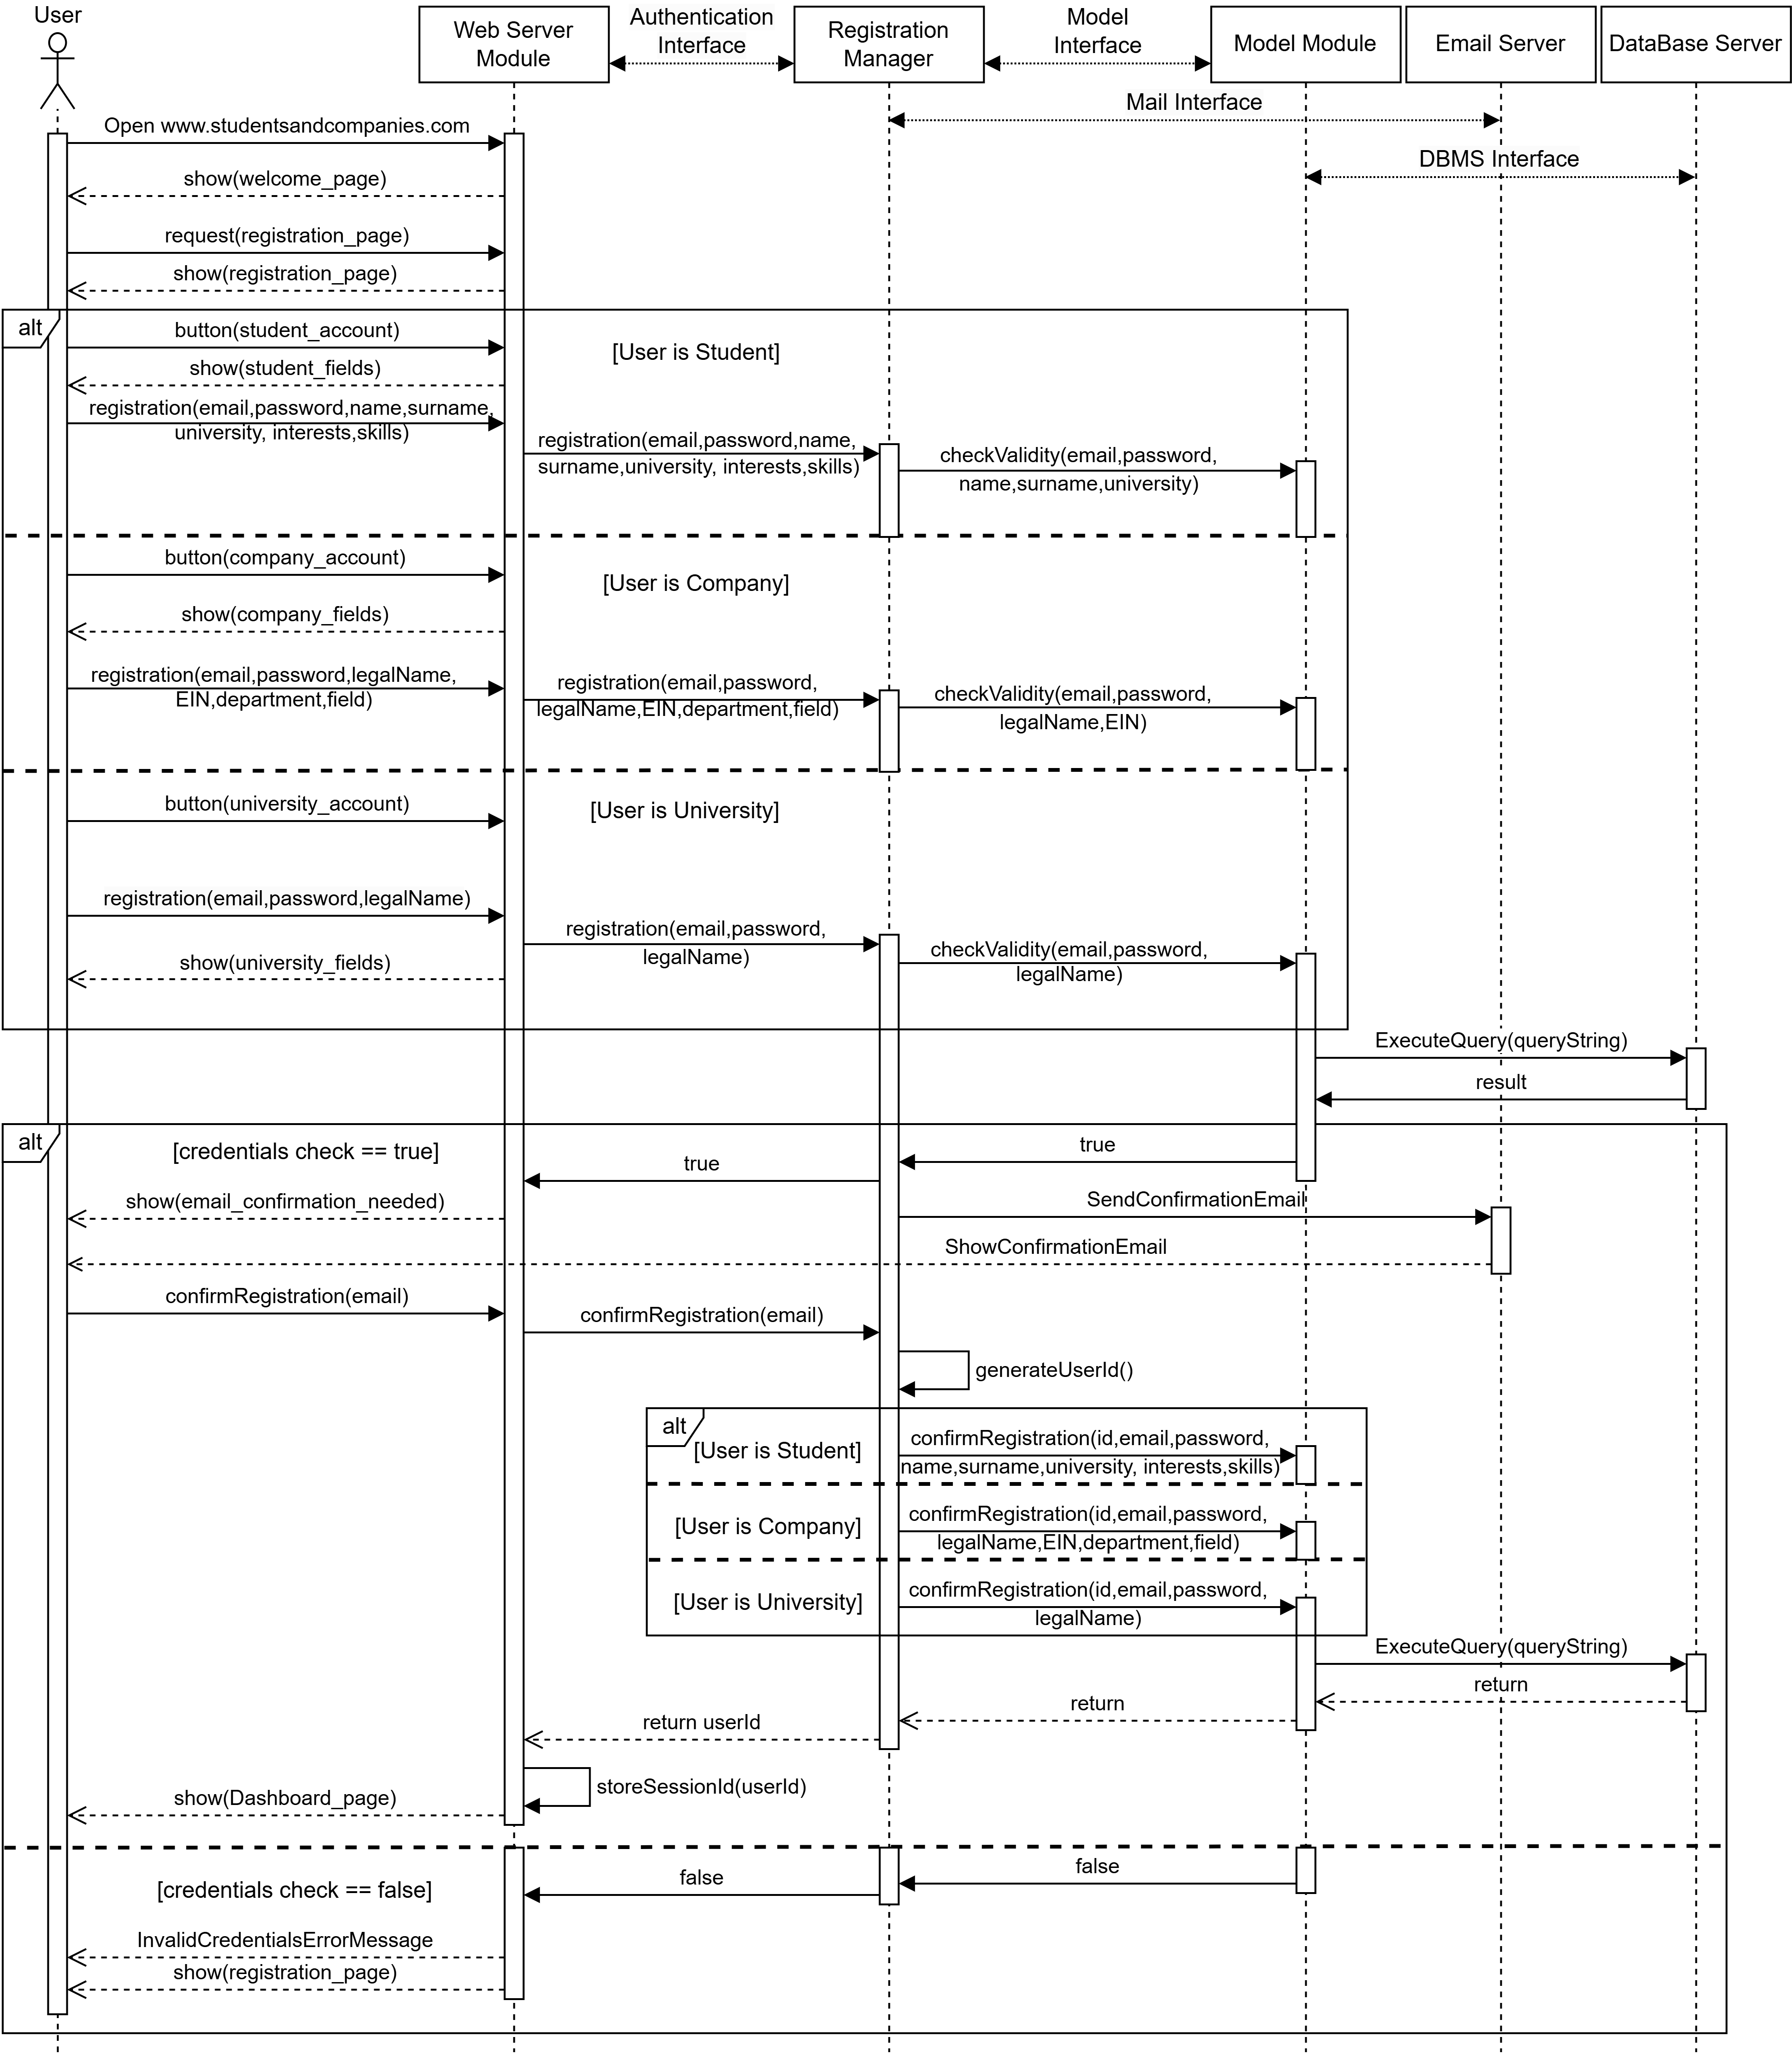
\includegraphics[width=1\textwidth]{Images/Runtime_view/registration_SD.png}
    \caption{Registration to S\&C Sequence Diagram}
\end{figure}
% Use Case 2
\begin{figure}[H]
    \centering
    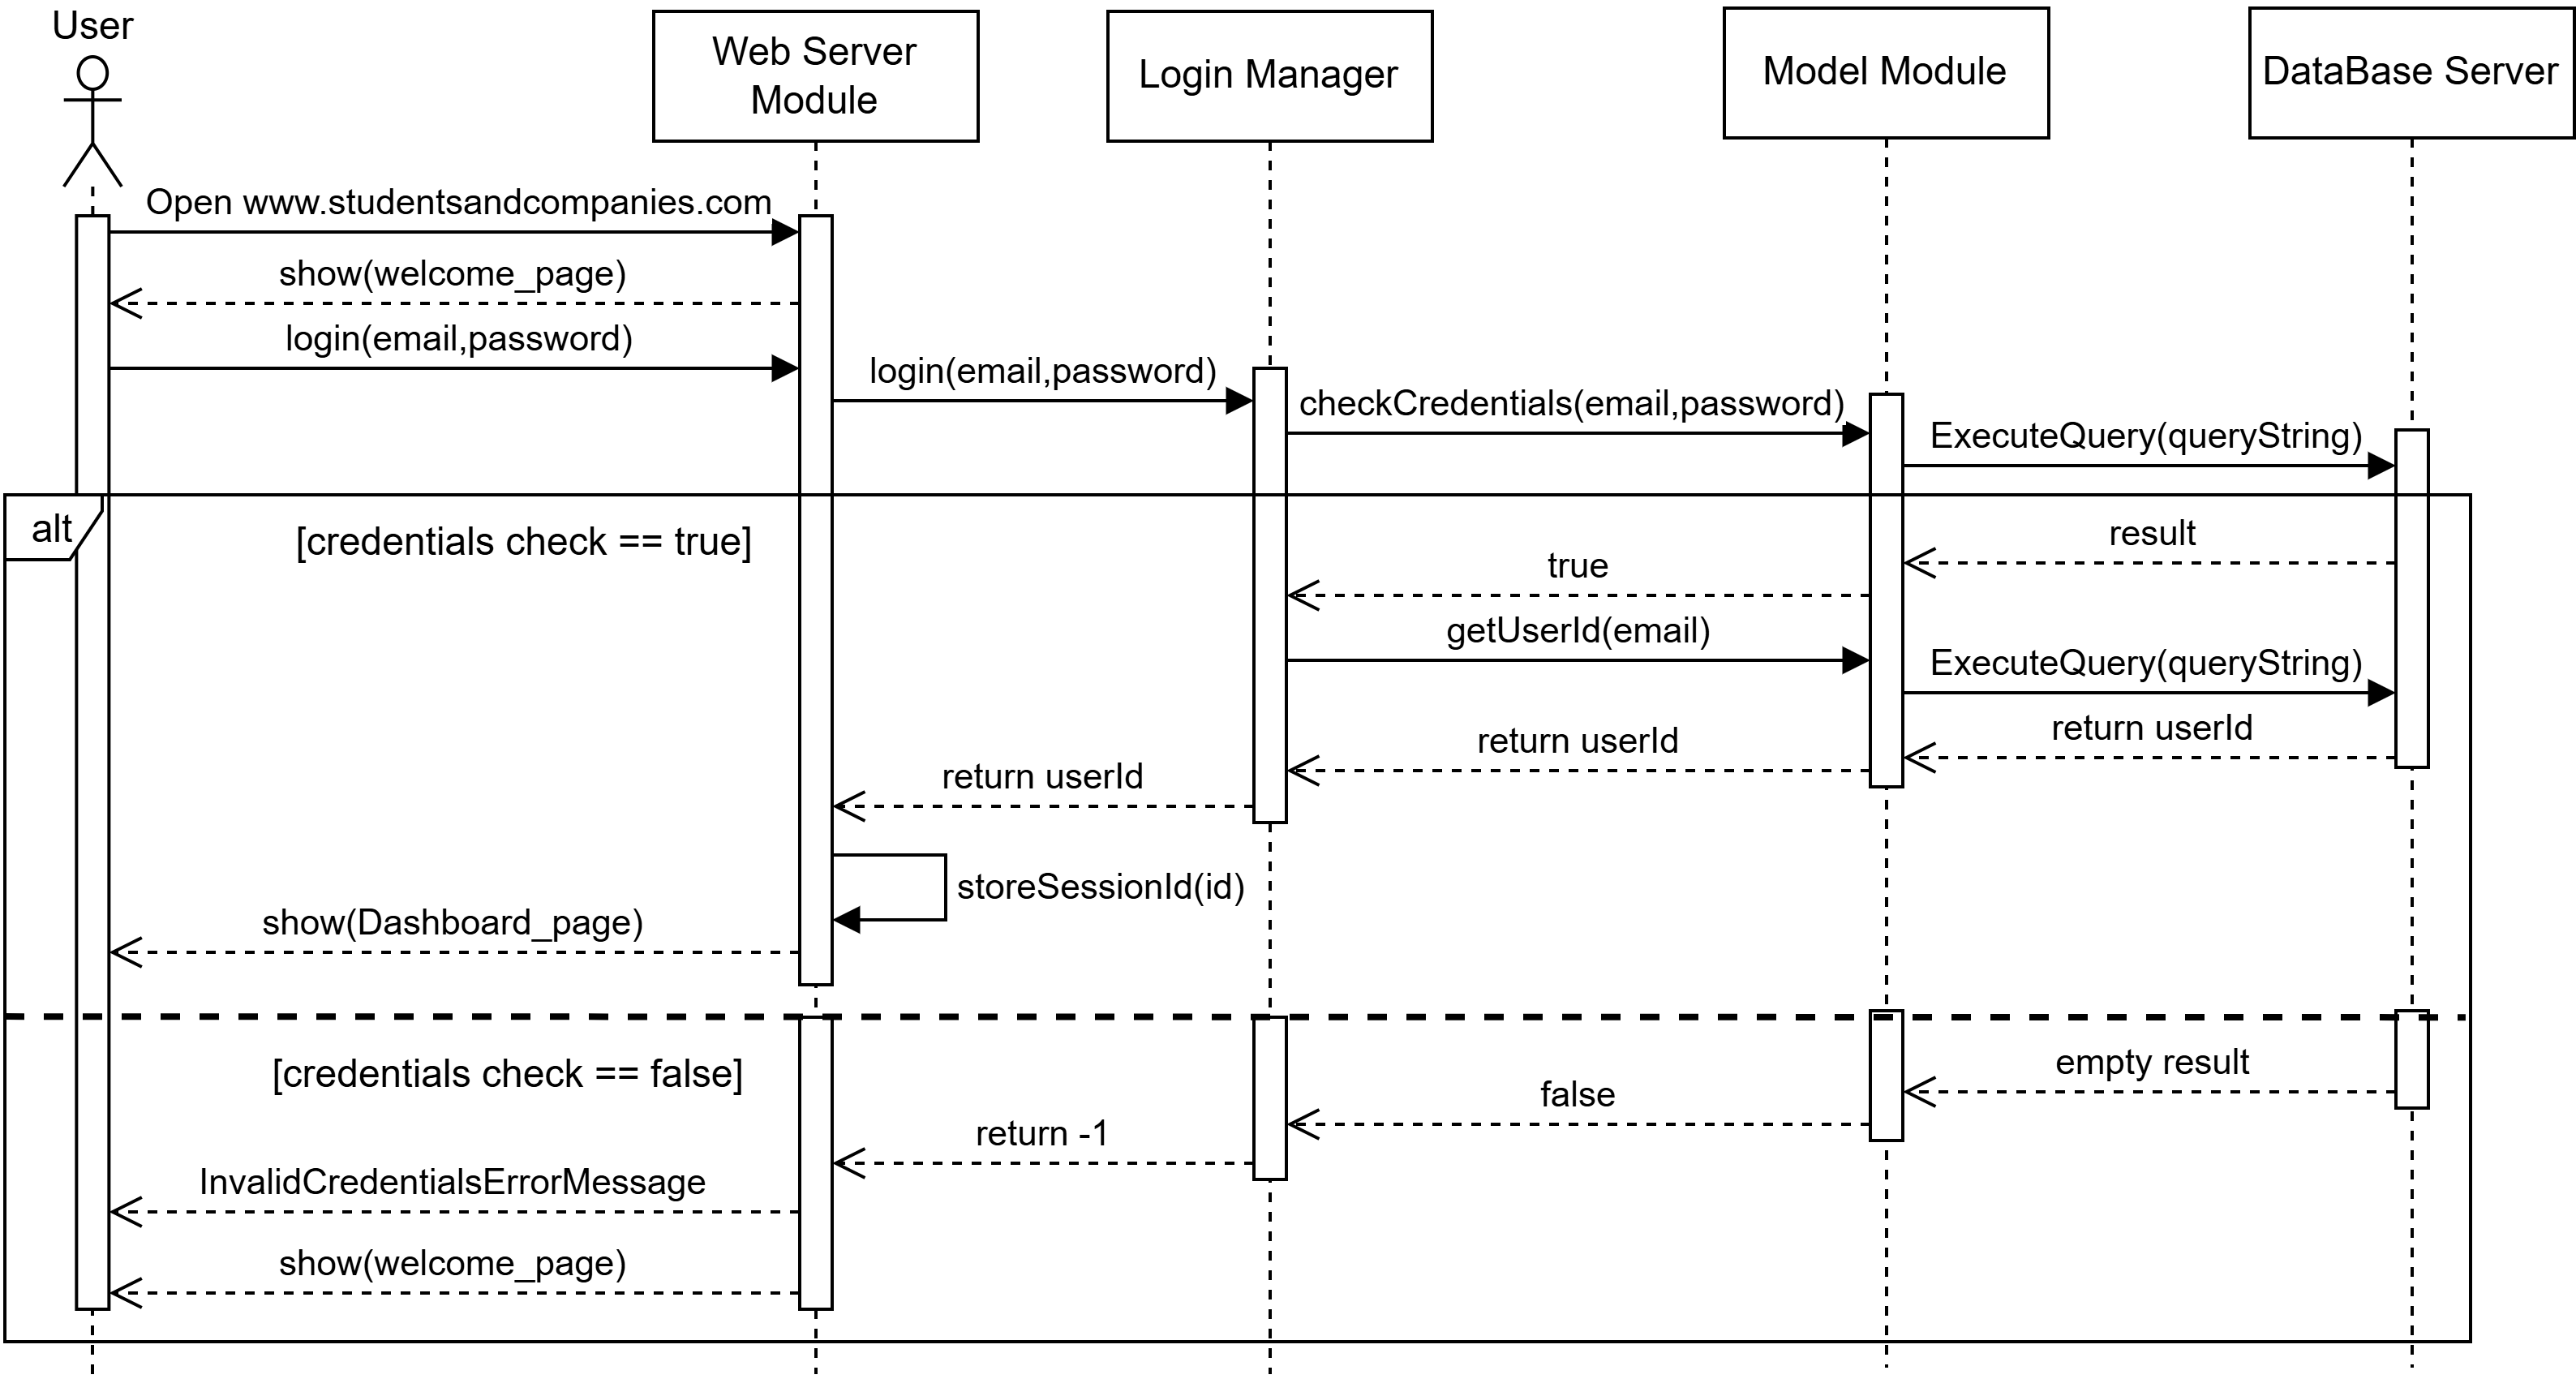
\includegraphics[width=1\textwidth]{Images/Runtime_view/login_SD.png}
    \caption{Login to S\&C Sequence Diagram}
\end{figure}
% Use Case 3
\begin{figure}[H]
    \centering
    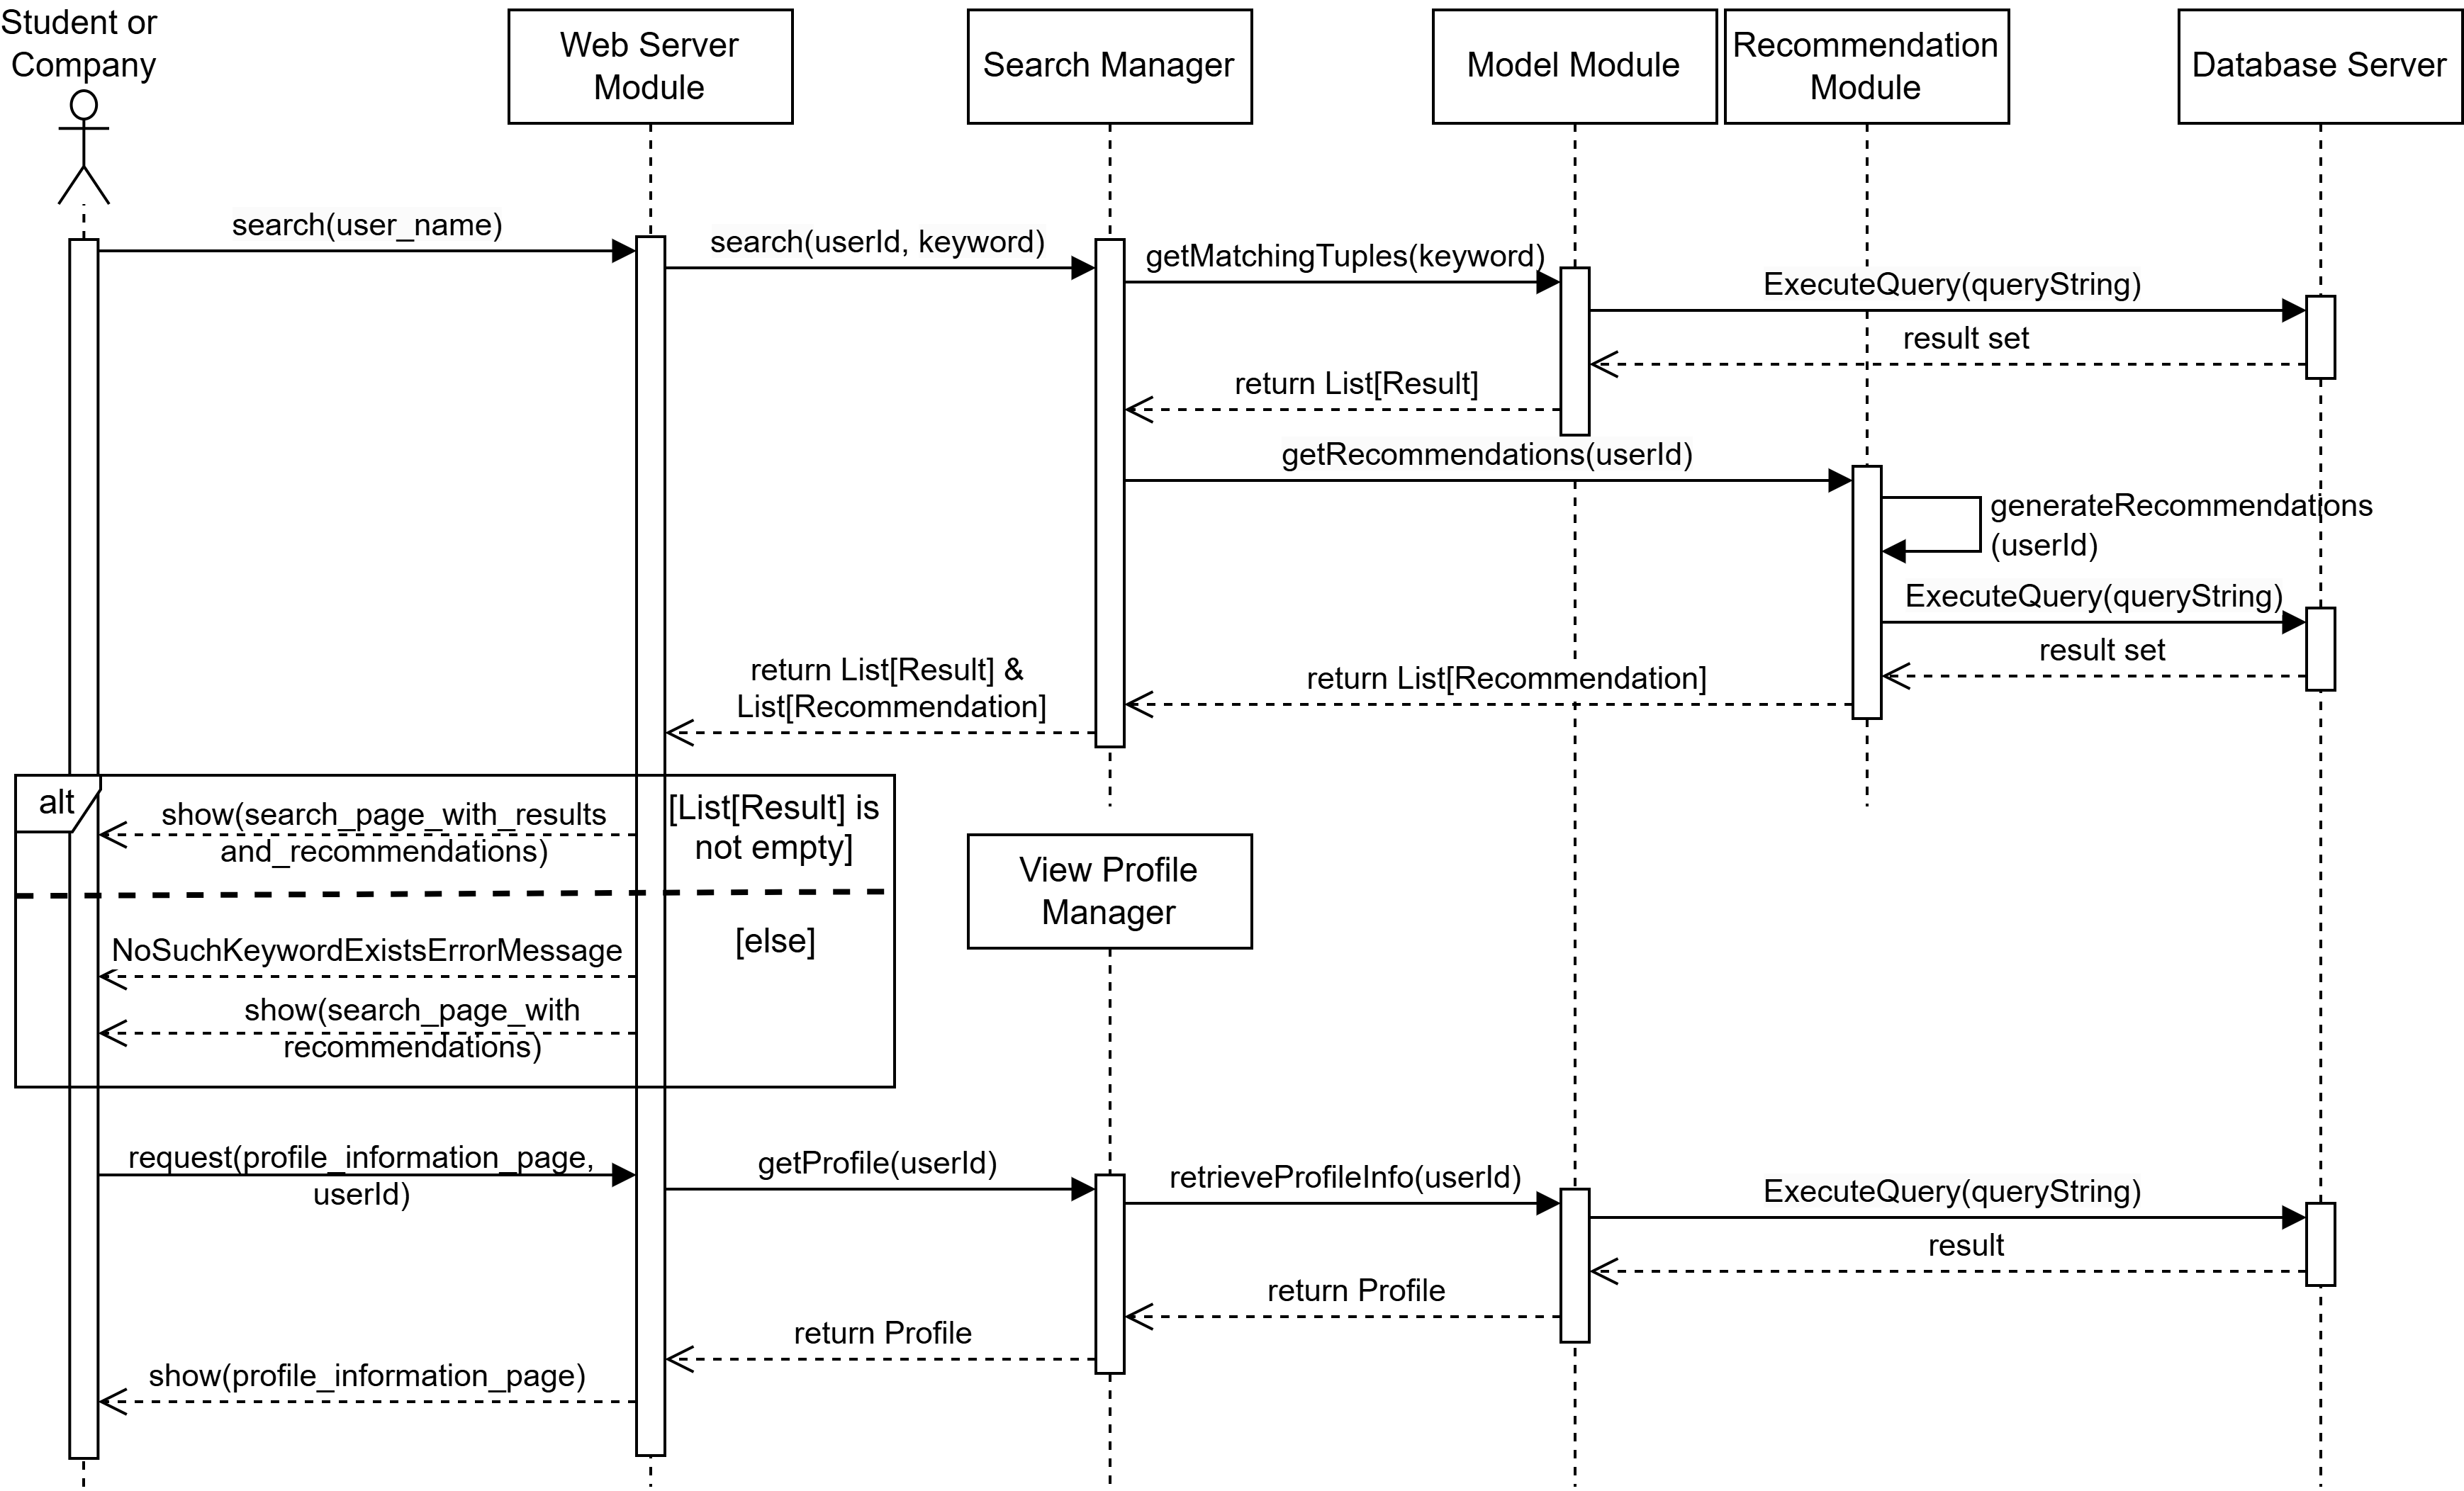
\includegraphics[width=1\textwidth]{Images/Runtime_view/seeProfile_SD.png}
    \caption{User sees profile information Sequence Diagram}
\end{figure}
% Use Case 4
\begin{figure}[H]
    \centering
    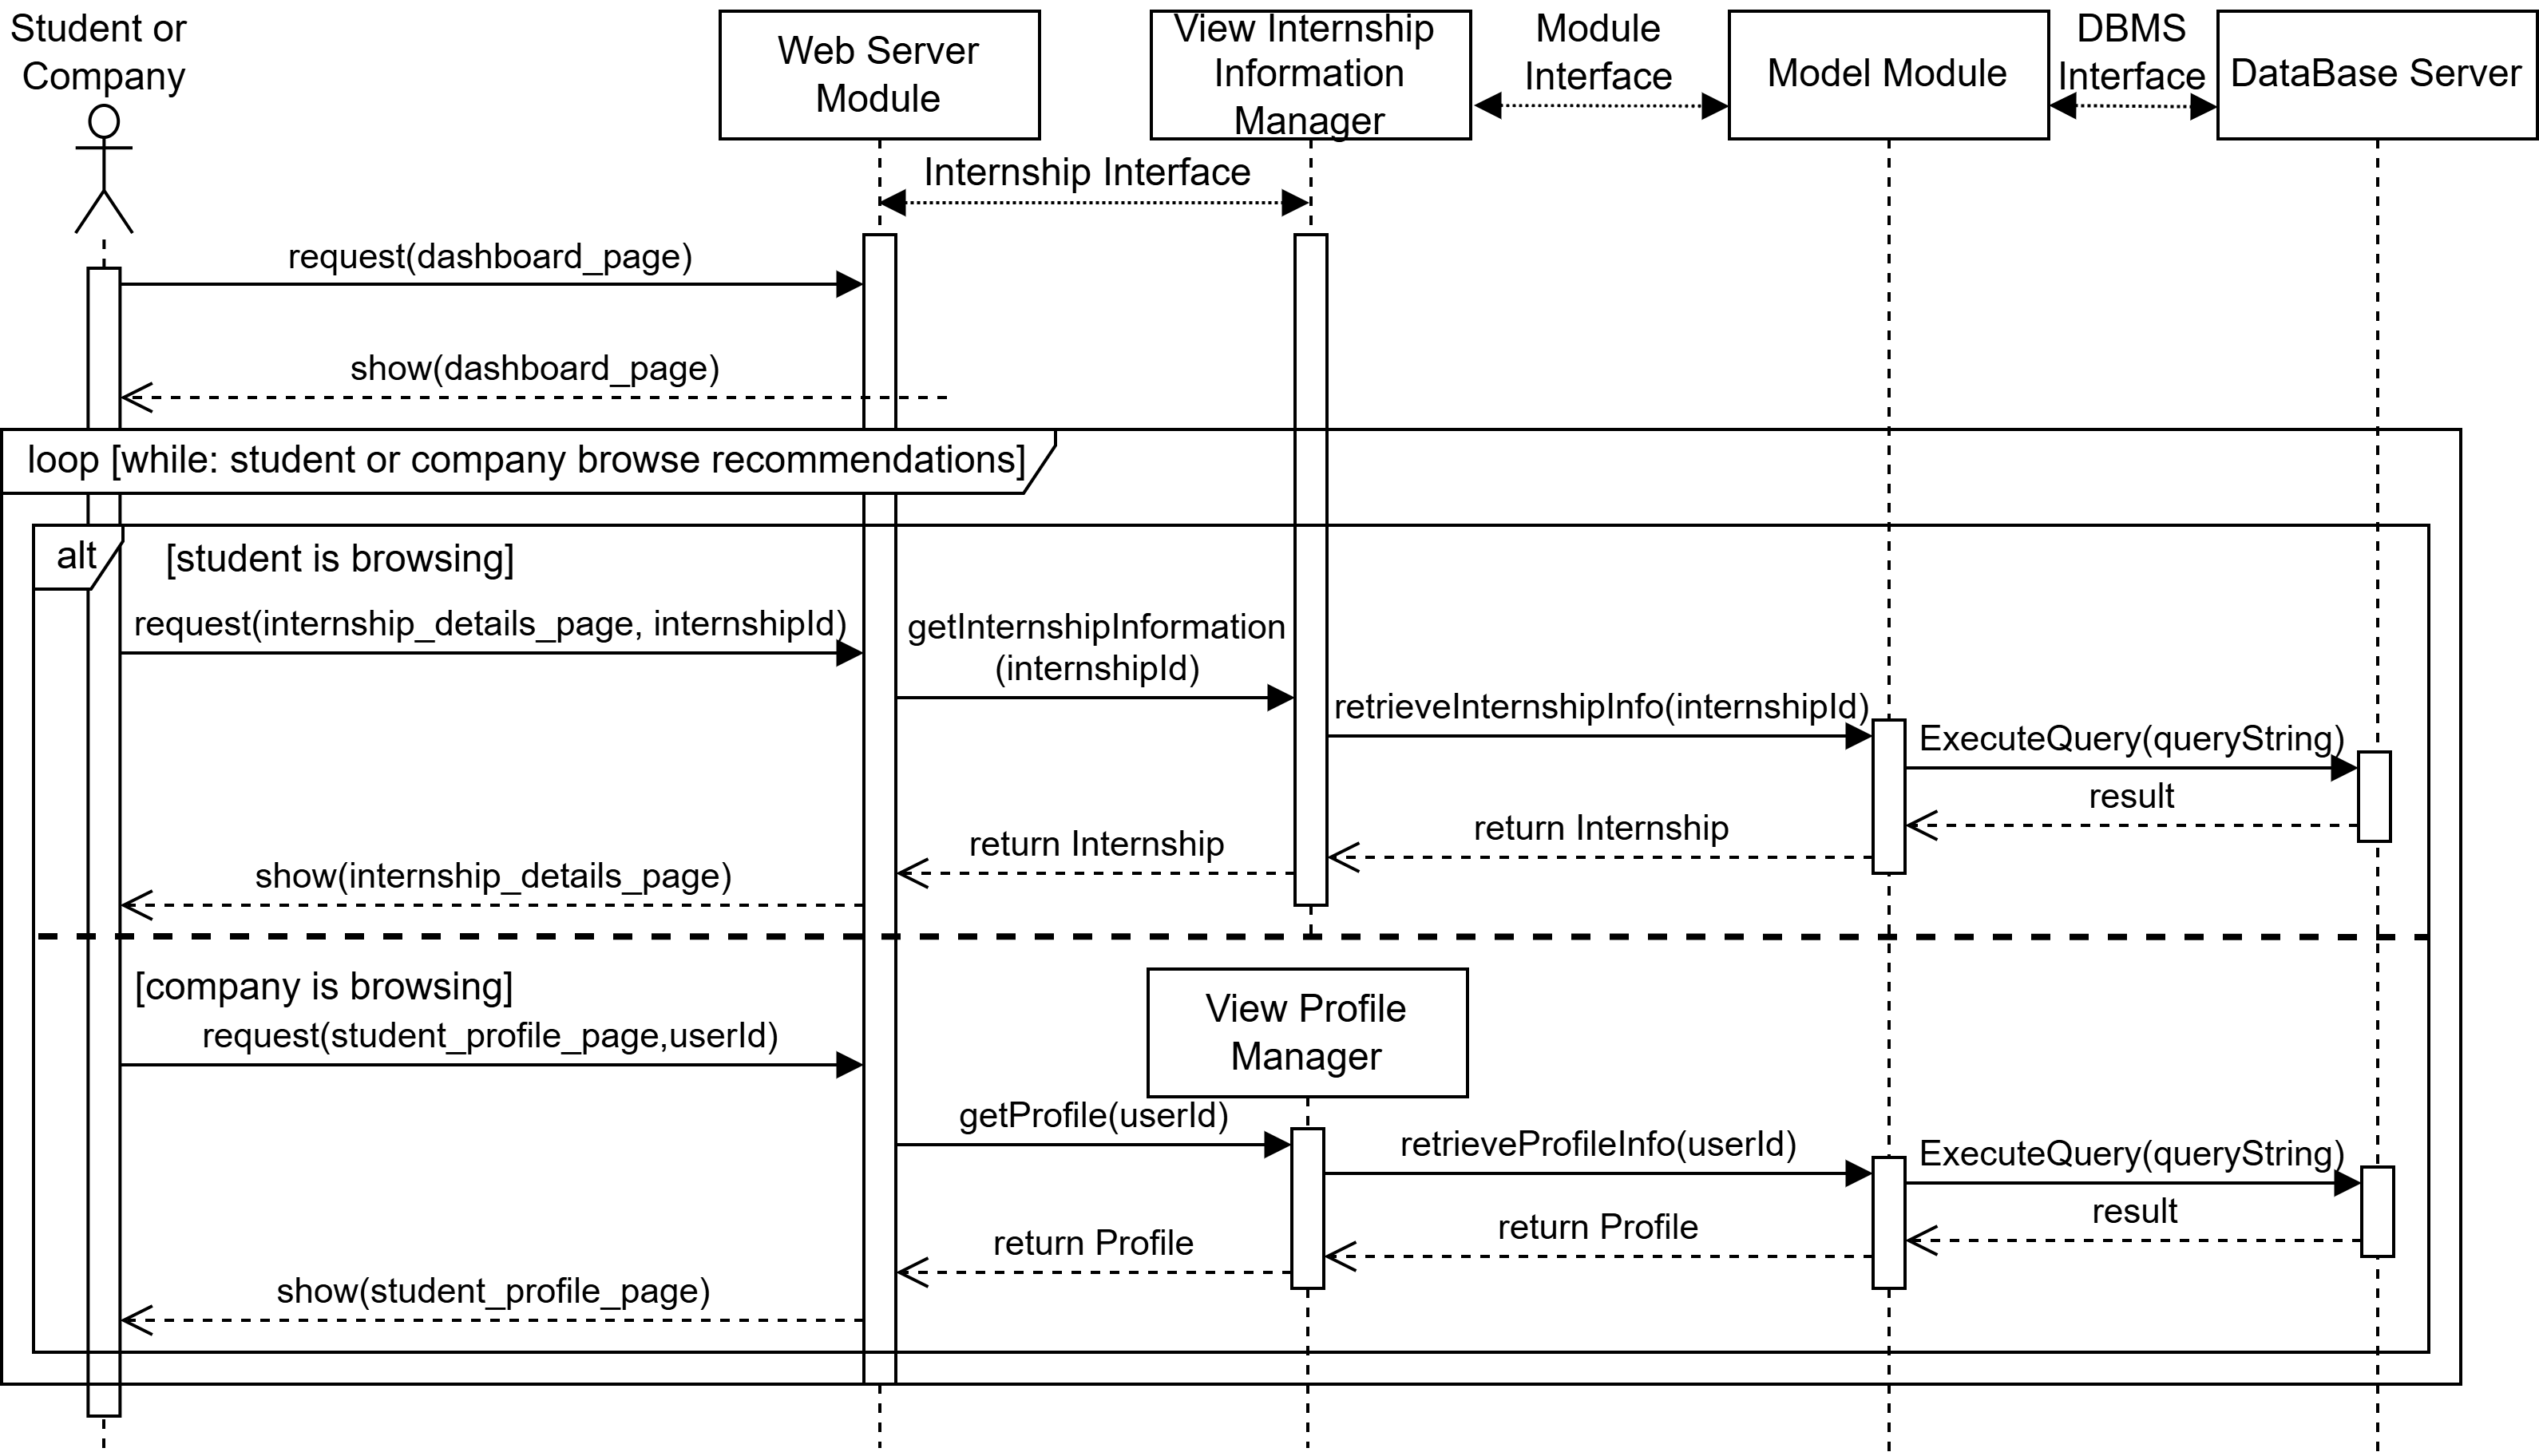
\includegraphics[width=1\textwidth]{Images/Runtime_view/recommendation_SD.png}
    \caption{Student or Company views recommendation Sequence Diagram}
\end{figure}
% Use Case 5
\begin{figure}[H]
    \centering
    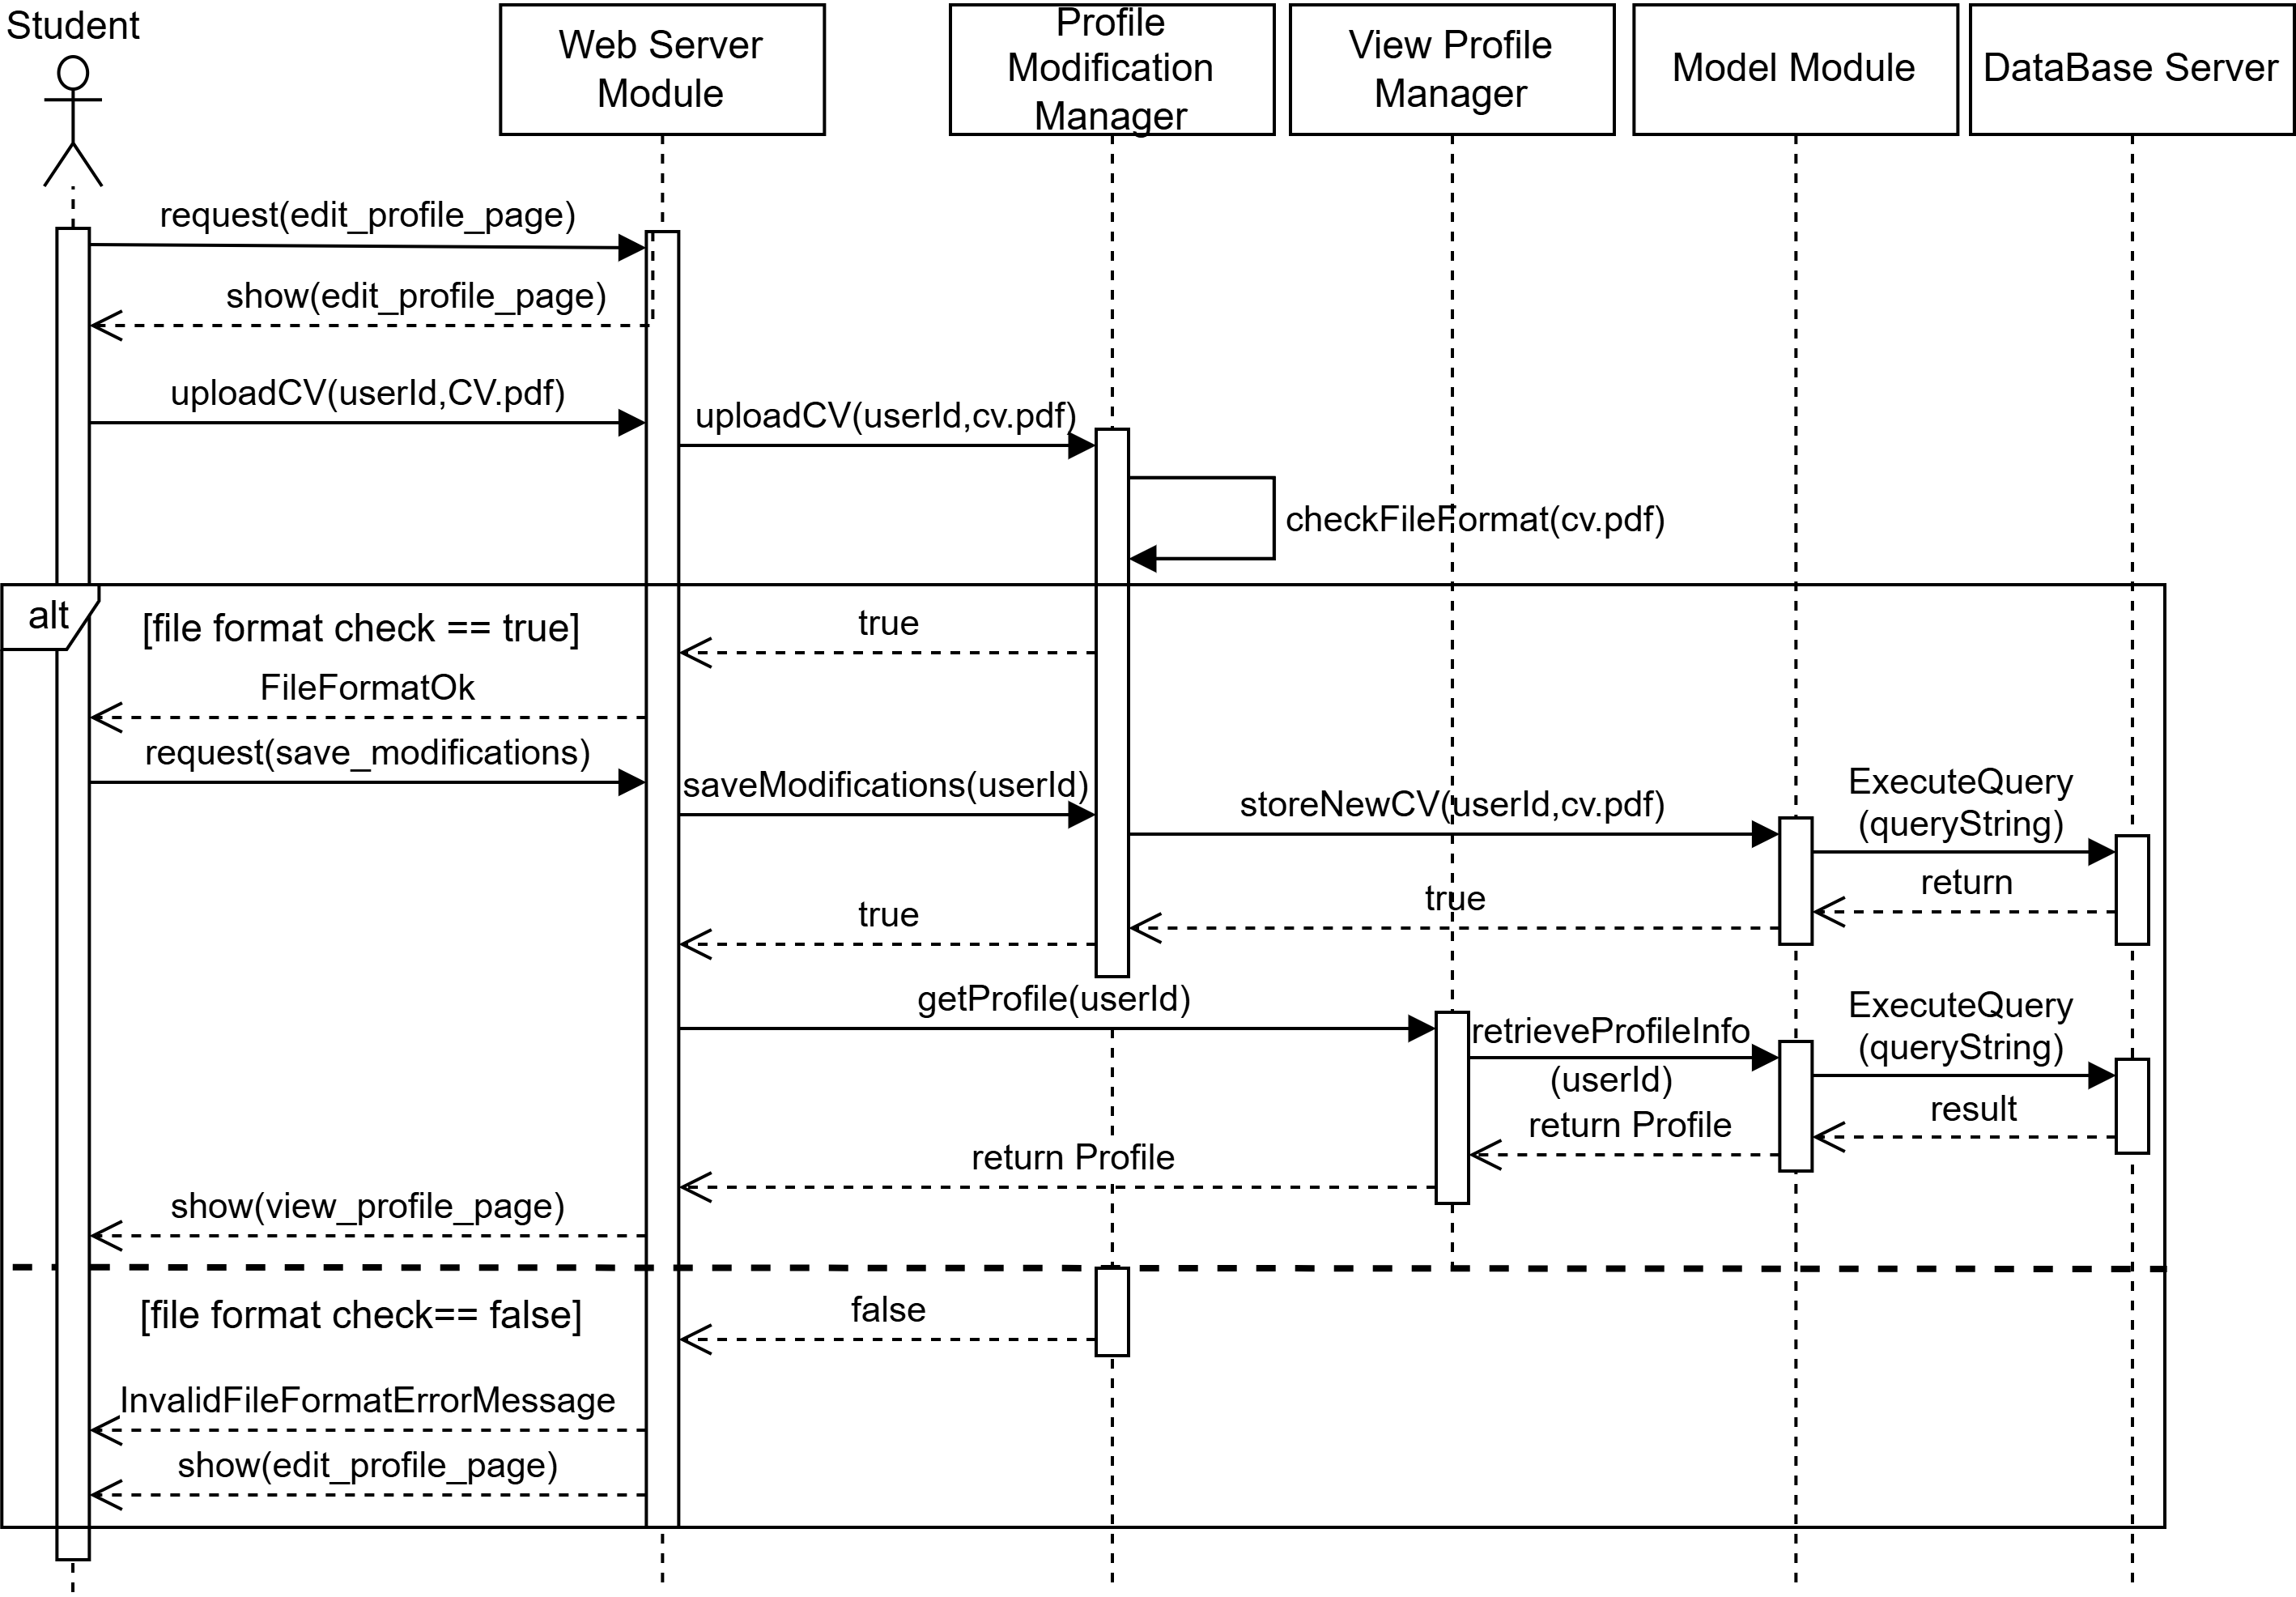
\includegraphics[width=1\textwidth]{Images/Runtime_view/uploadCV_SD.png}
    \caption{Student uploads CV to his profile Sequence Diagram}
\end{figure}
% Use Case 6
\begin{figure}[H]
    \centering
    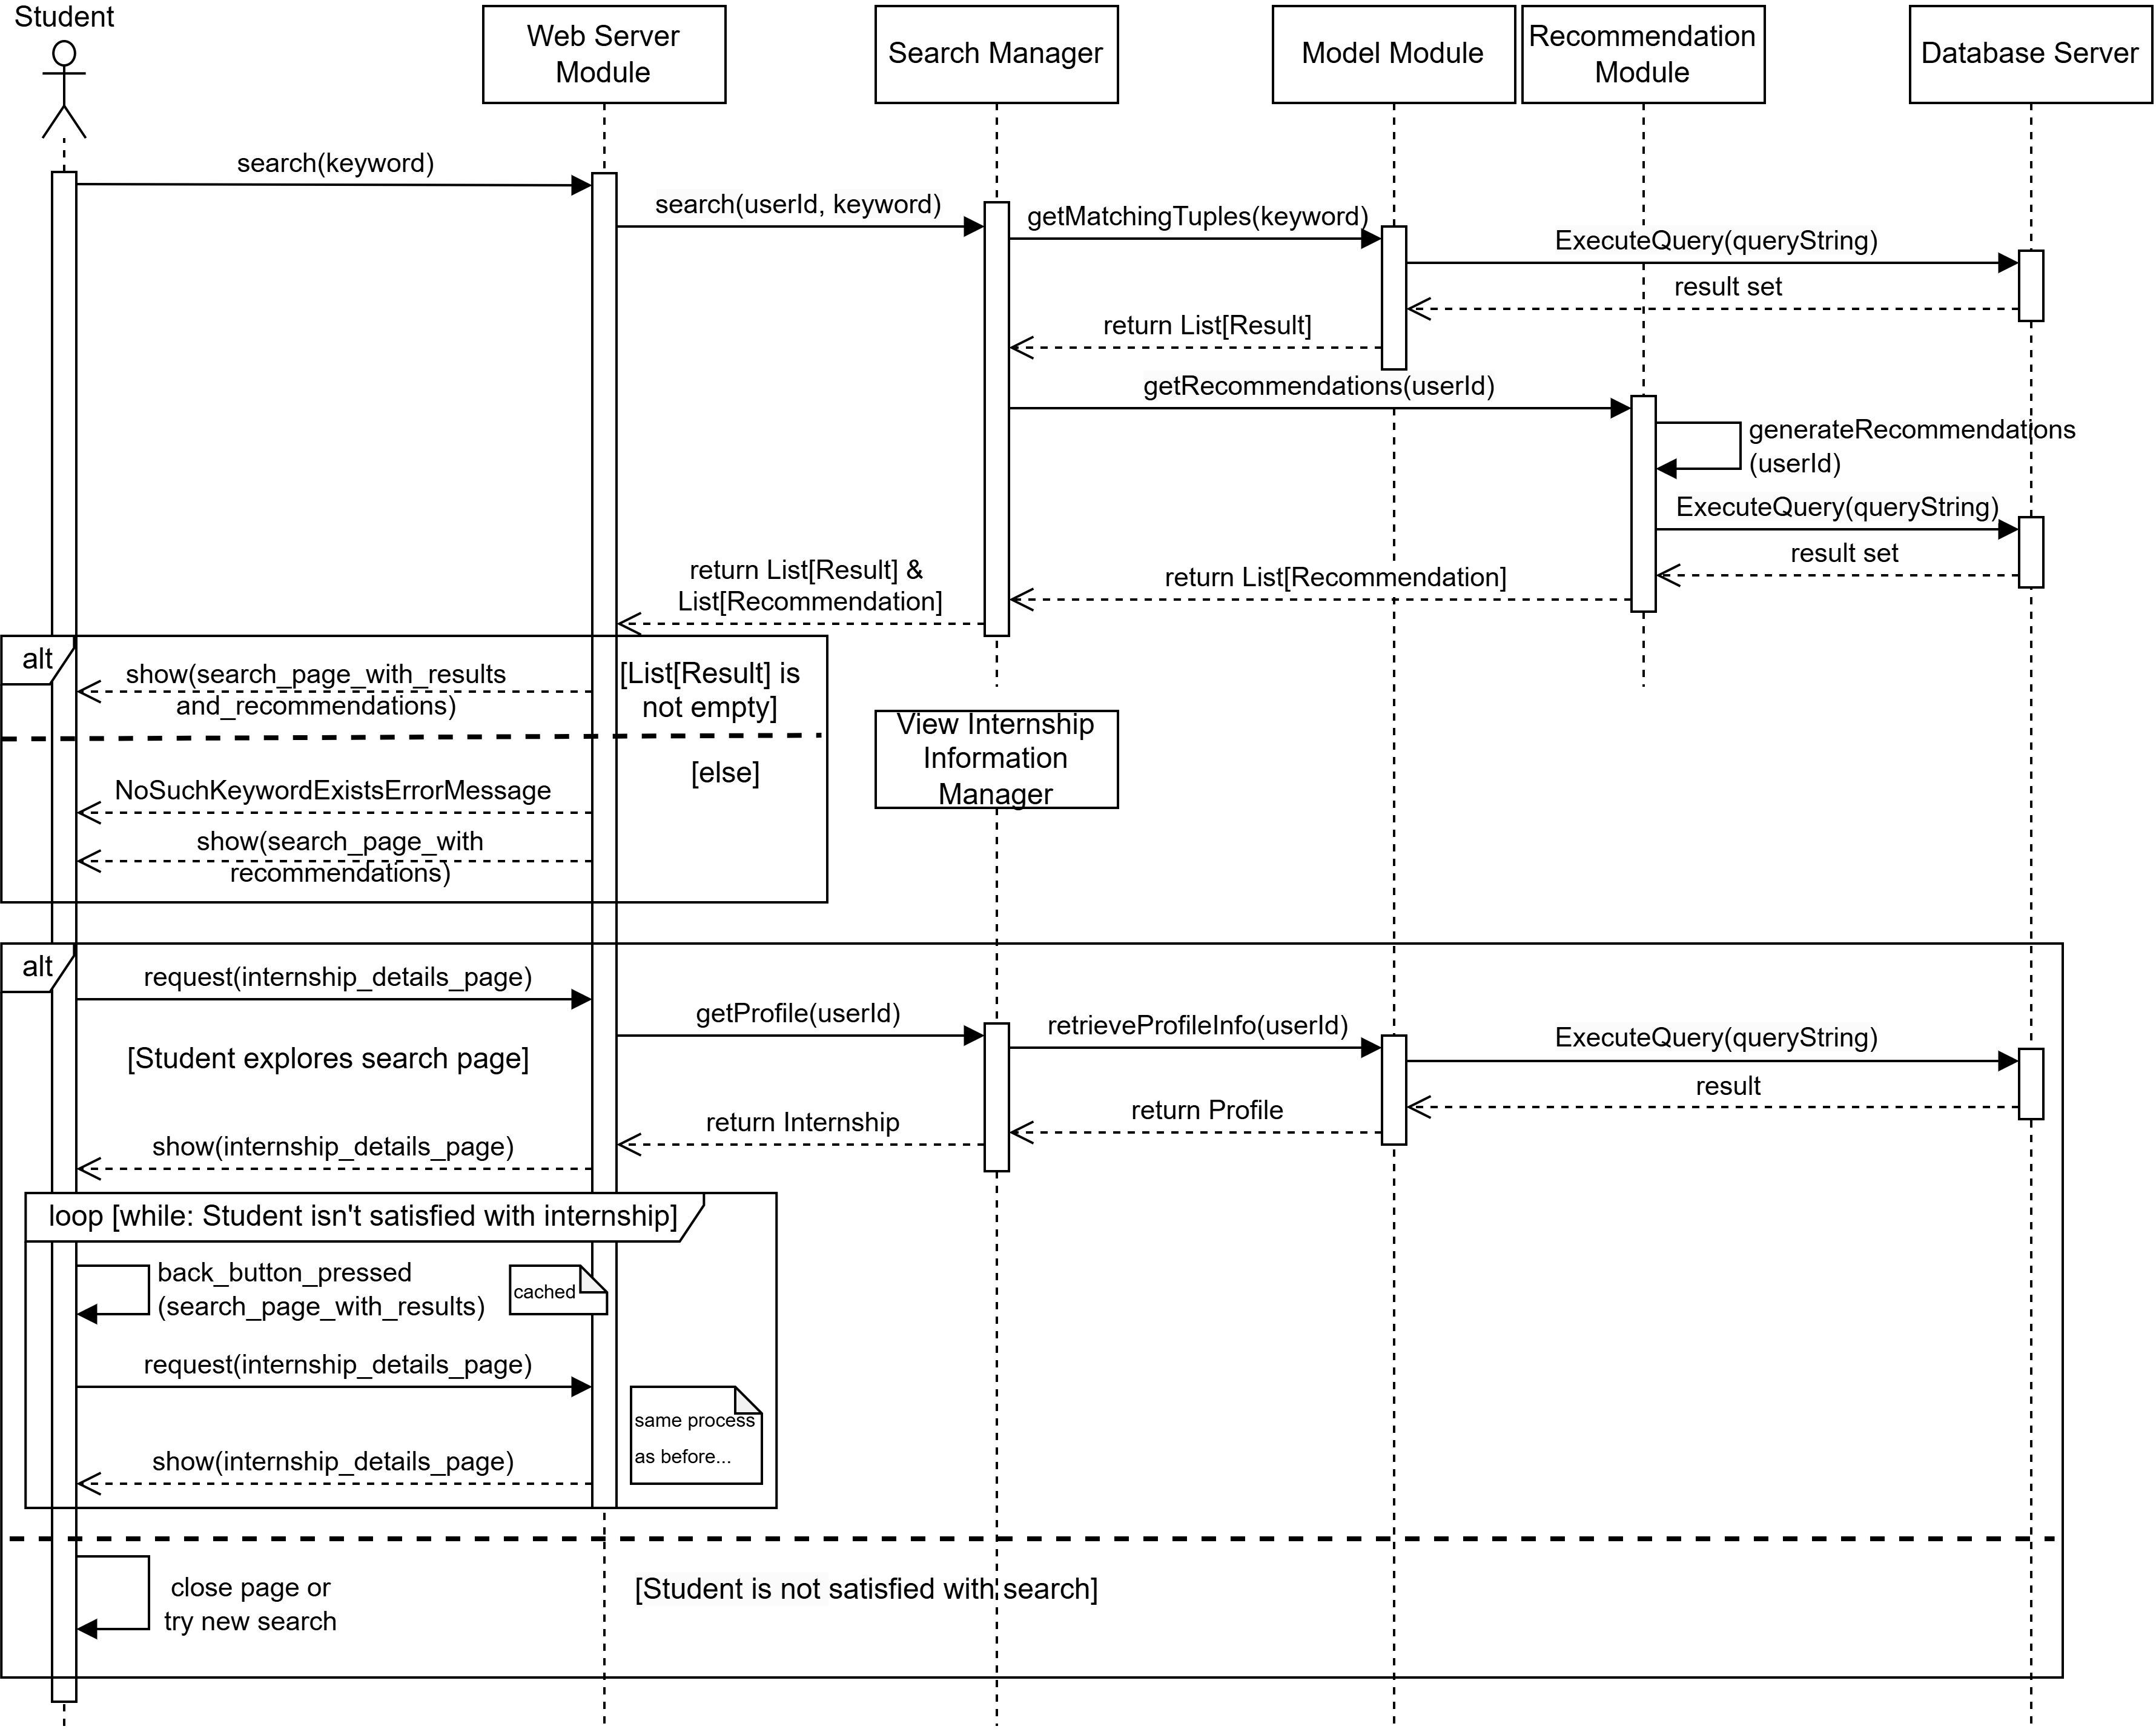
\includegraphics[width=1\textwidth]{Images/Runtime_view/searchInt_SD.png}
    \caption{Student searches for an internship Sequence Diagram}
\end{figure}
% Use Case 7
\begin{figure}[H]
    \centering
    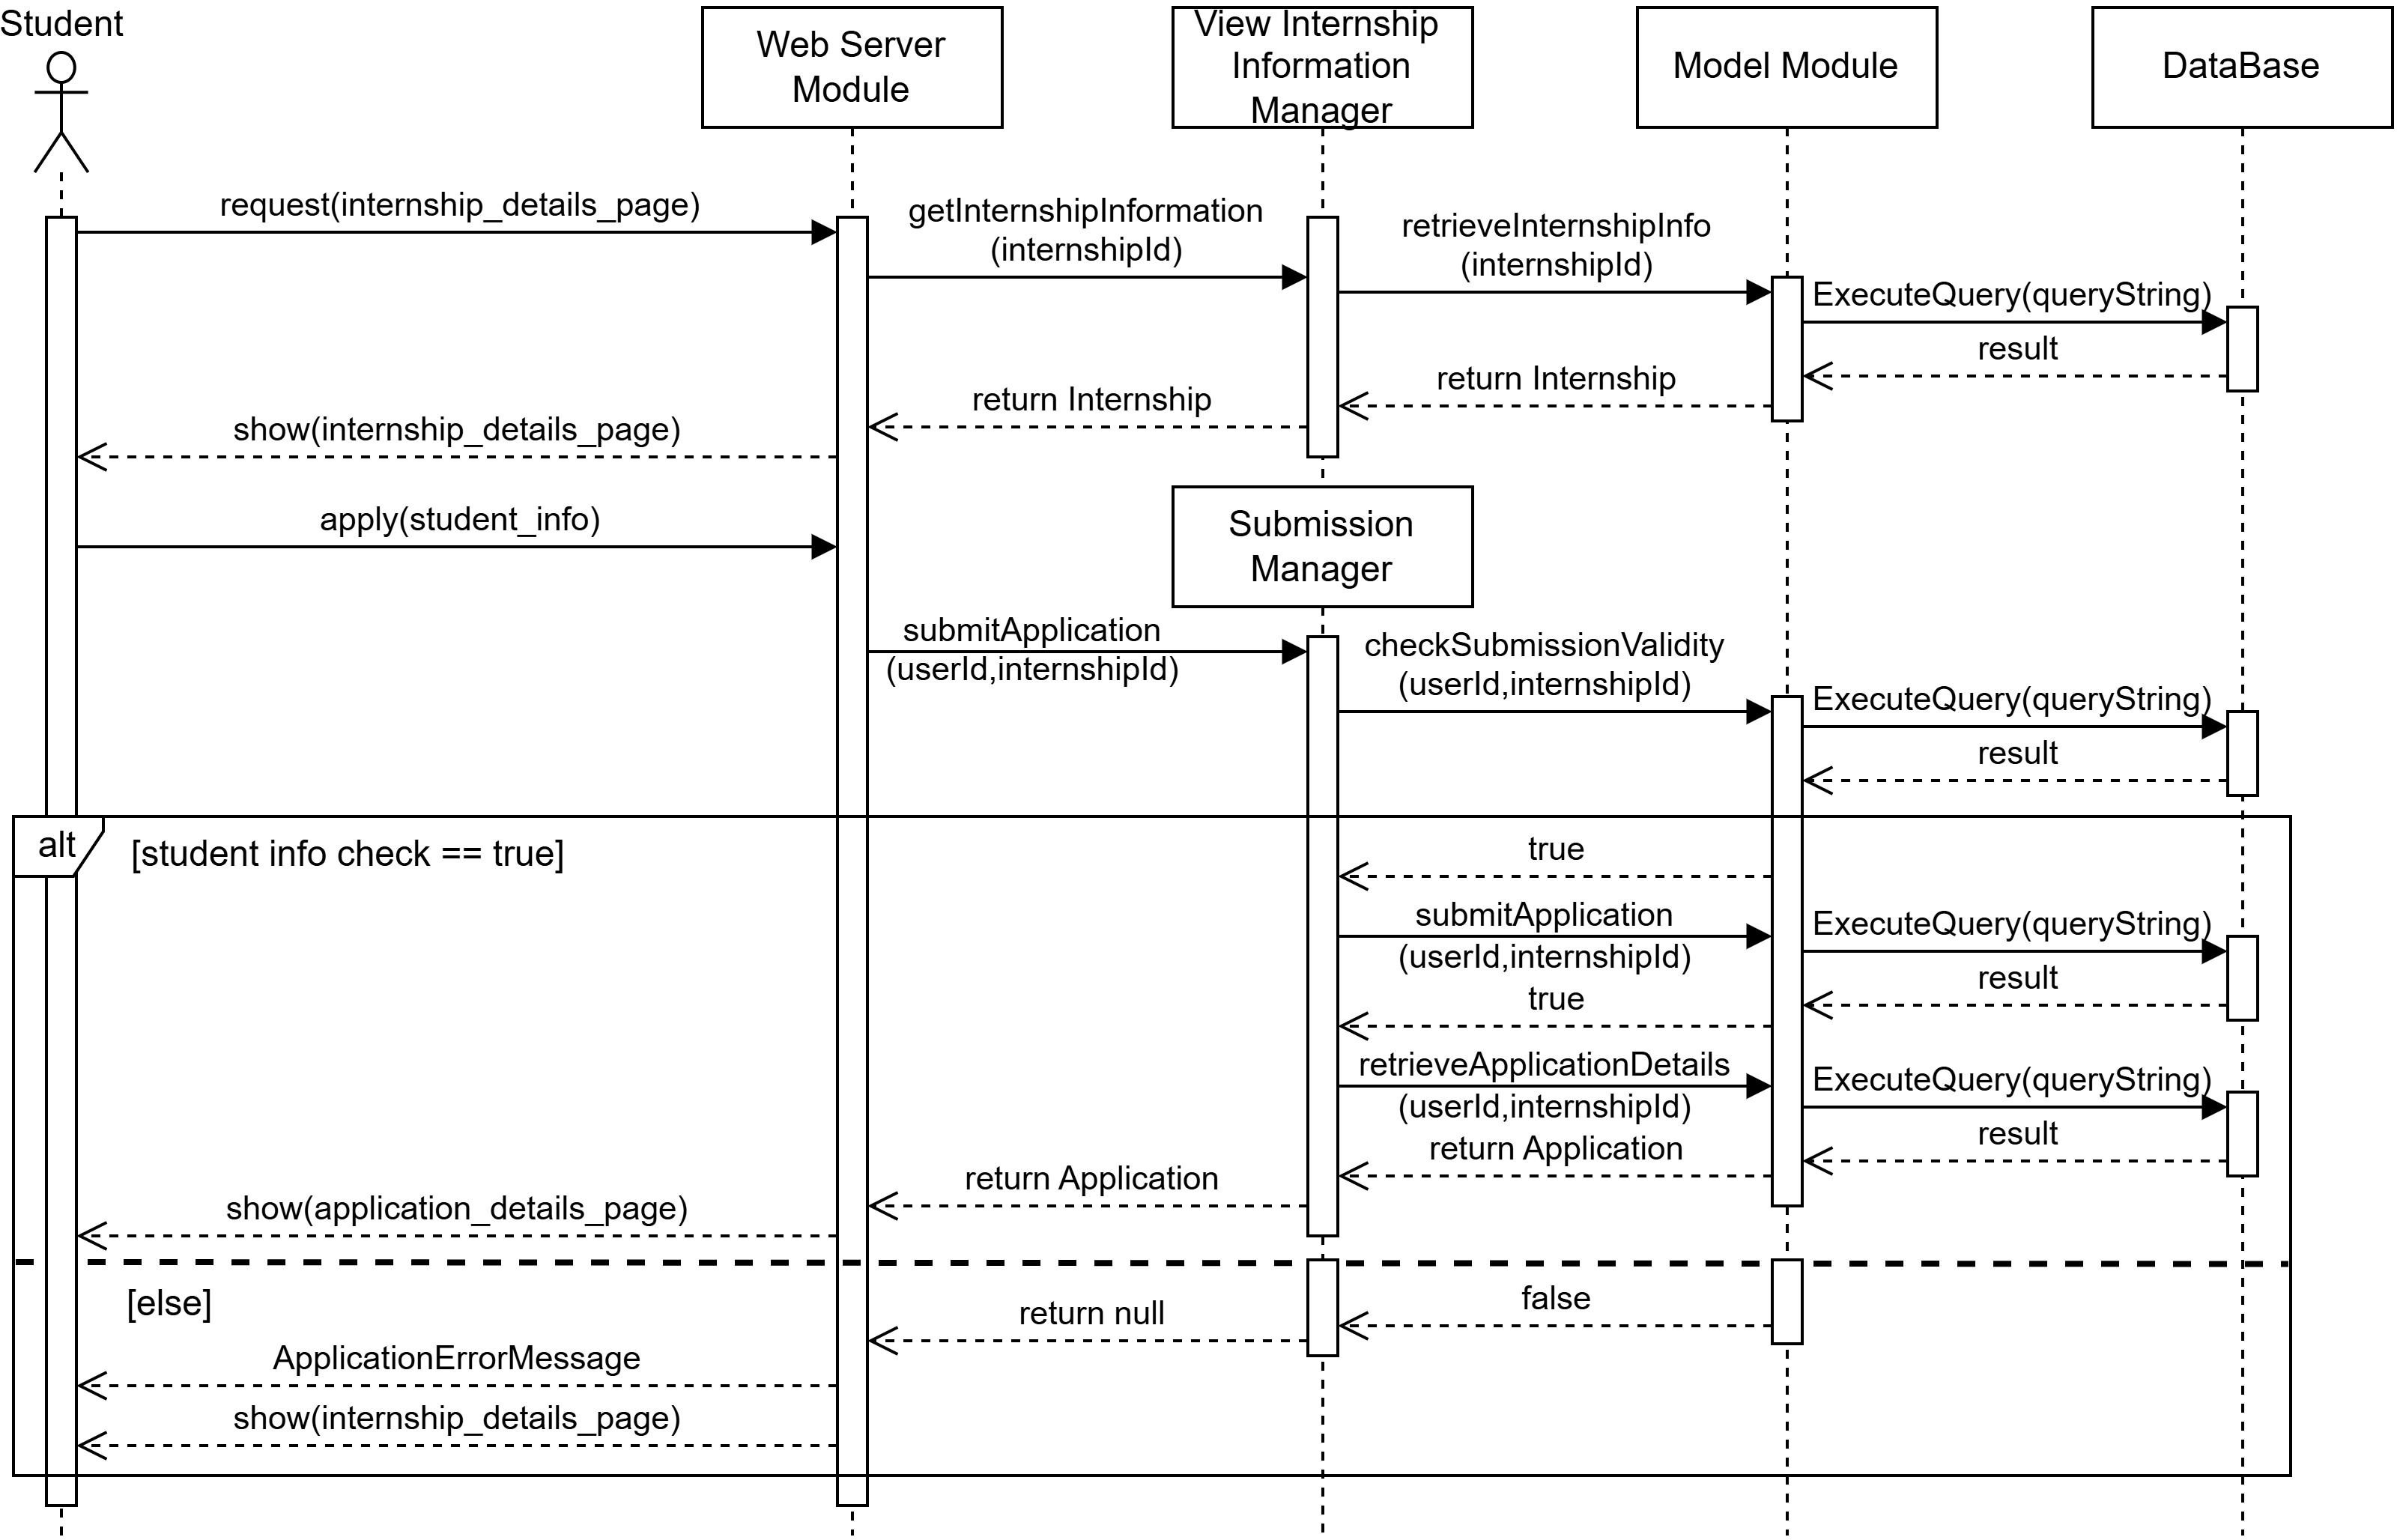
\includegraphics[width=1\textwidth]{Images/Runtime_view/applyInt_SD.png}
    \caption{Student applies for an internship Sequence Diagram}
\end{figure}
% Use Case 8
\begin{figure}[H]
    \centering
    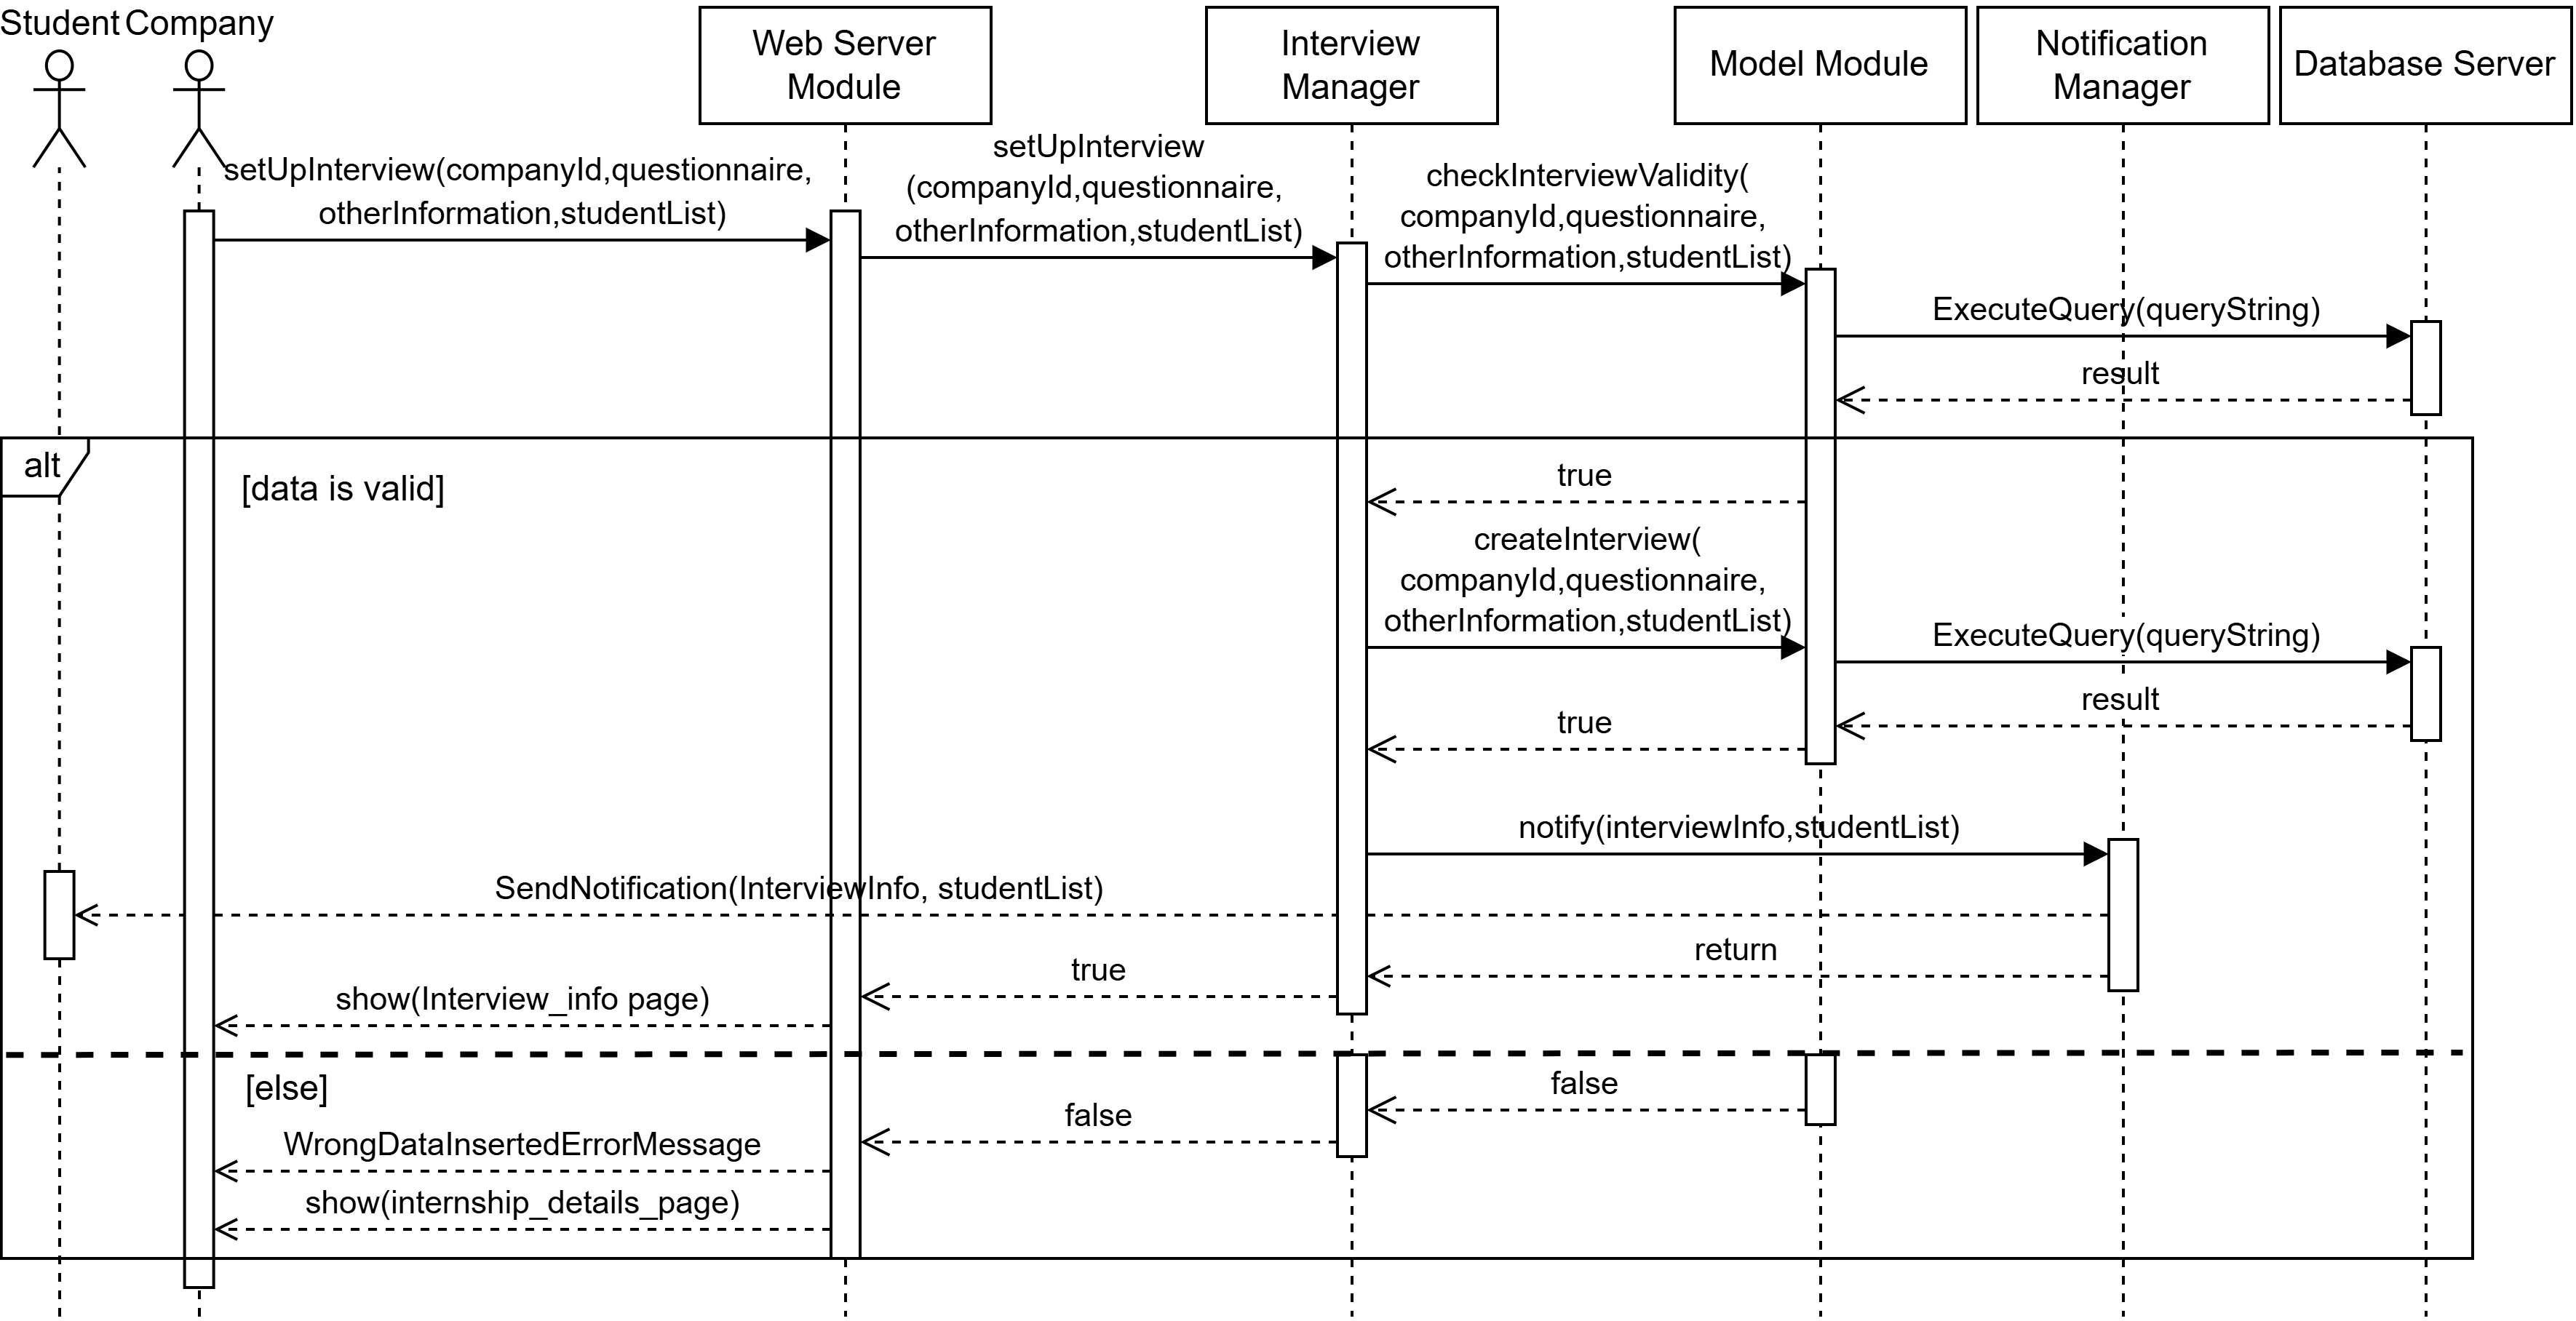
\includegraphics[width=1\textwidth]{Images/Runtime_view/createIntvw_SD.png}
    \caption{Company creates an interview Sequence Diagram}
\end{figure}
% Use Case 9
\begin{figure}[H]
    \centering
    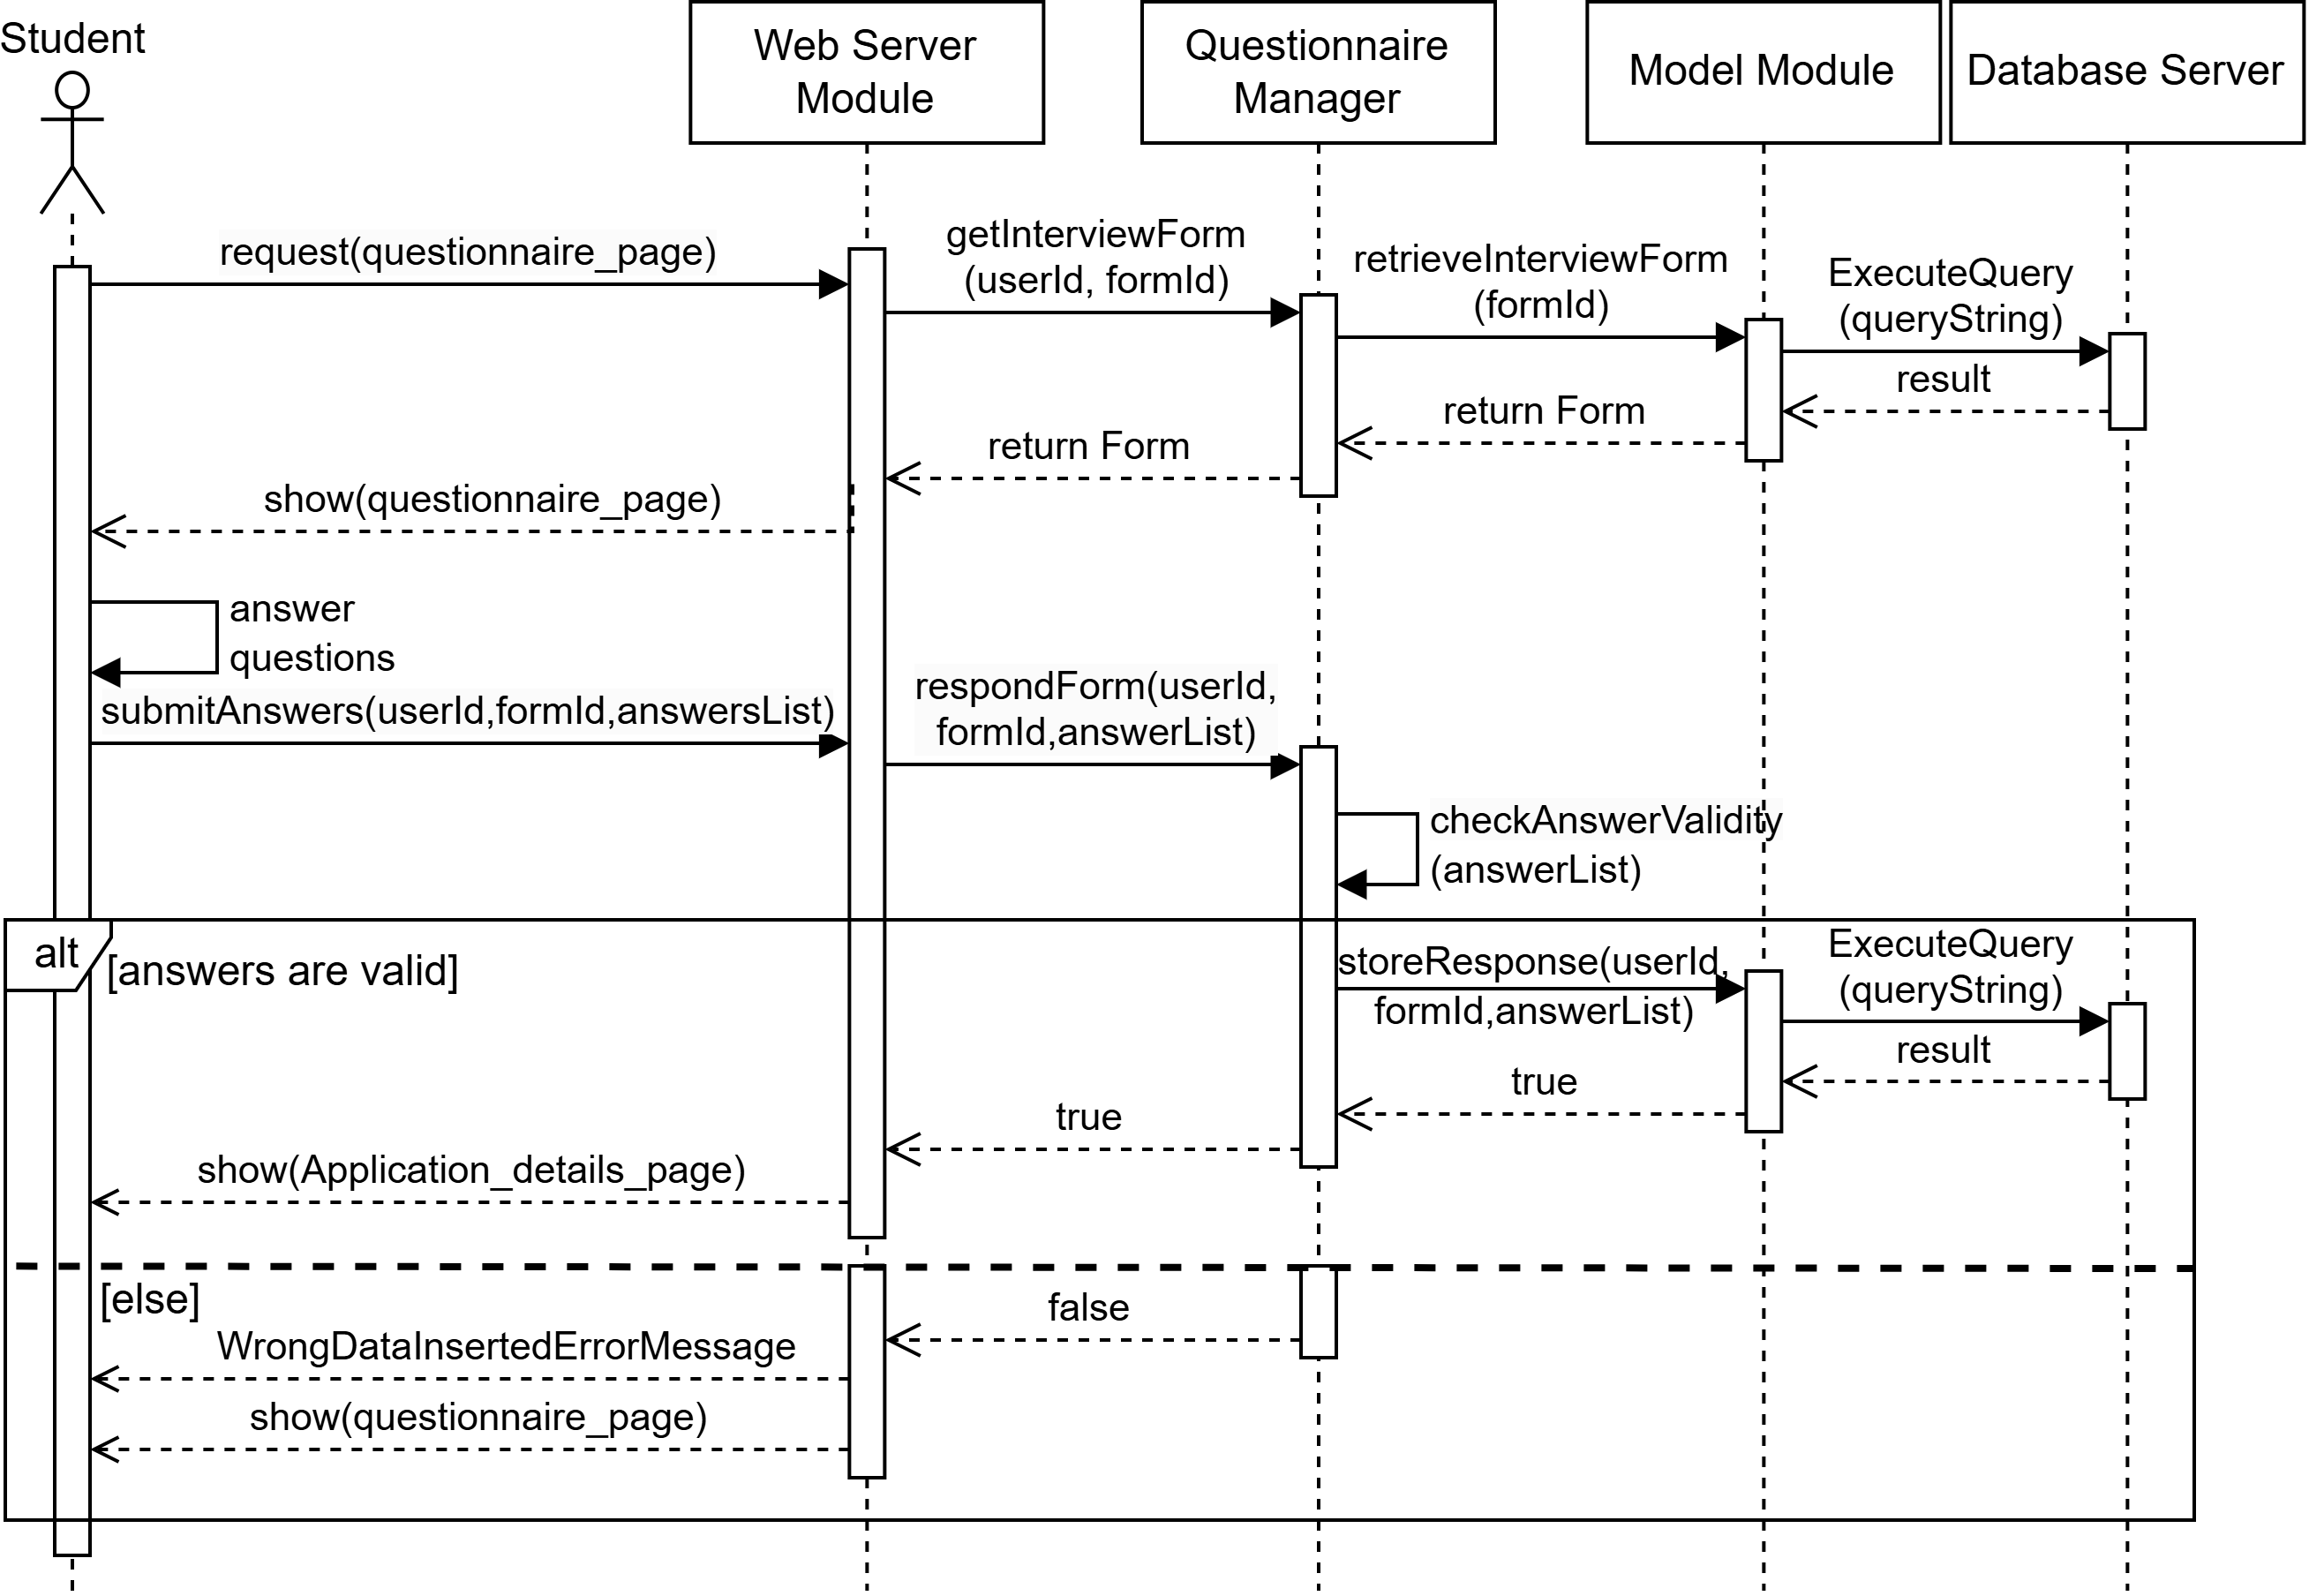
\includegraphics[width=1\textwidth]{Images/Runtime_view/respondQuest_SD.png}
    \caption{Student responds to an interview questionnaire Sequence Diagram}
\end{figure}
% Use Case 10
\begin{figure}[H]
    \centering
    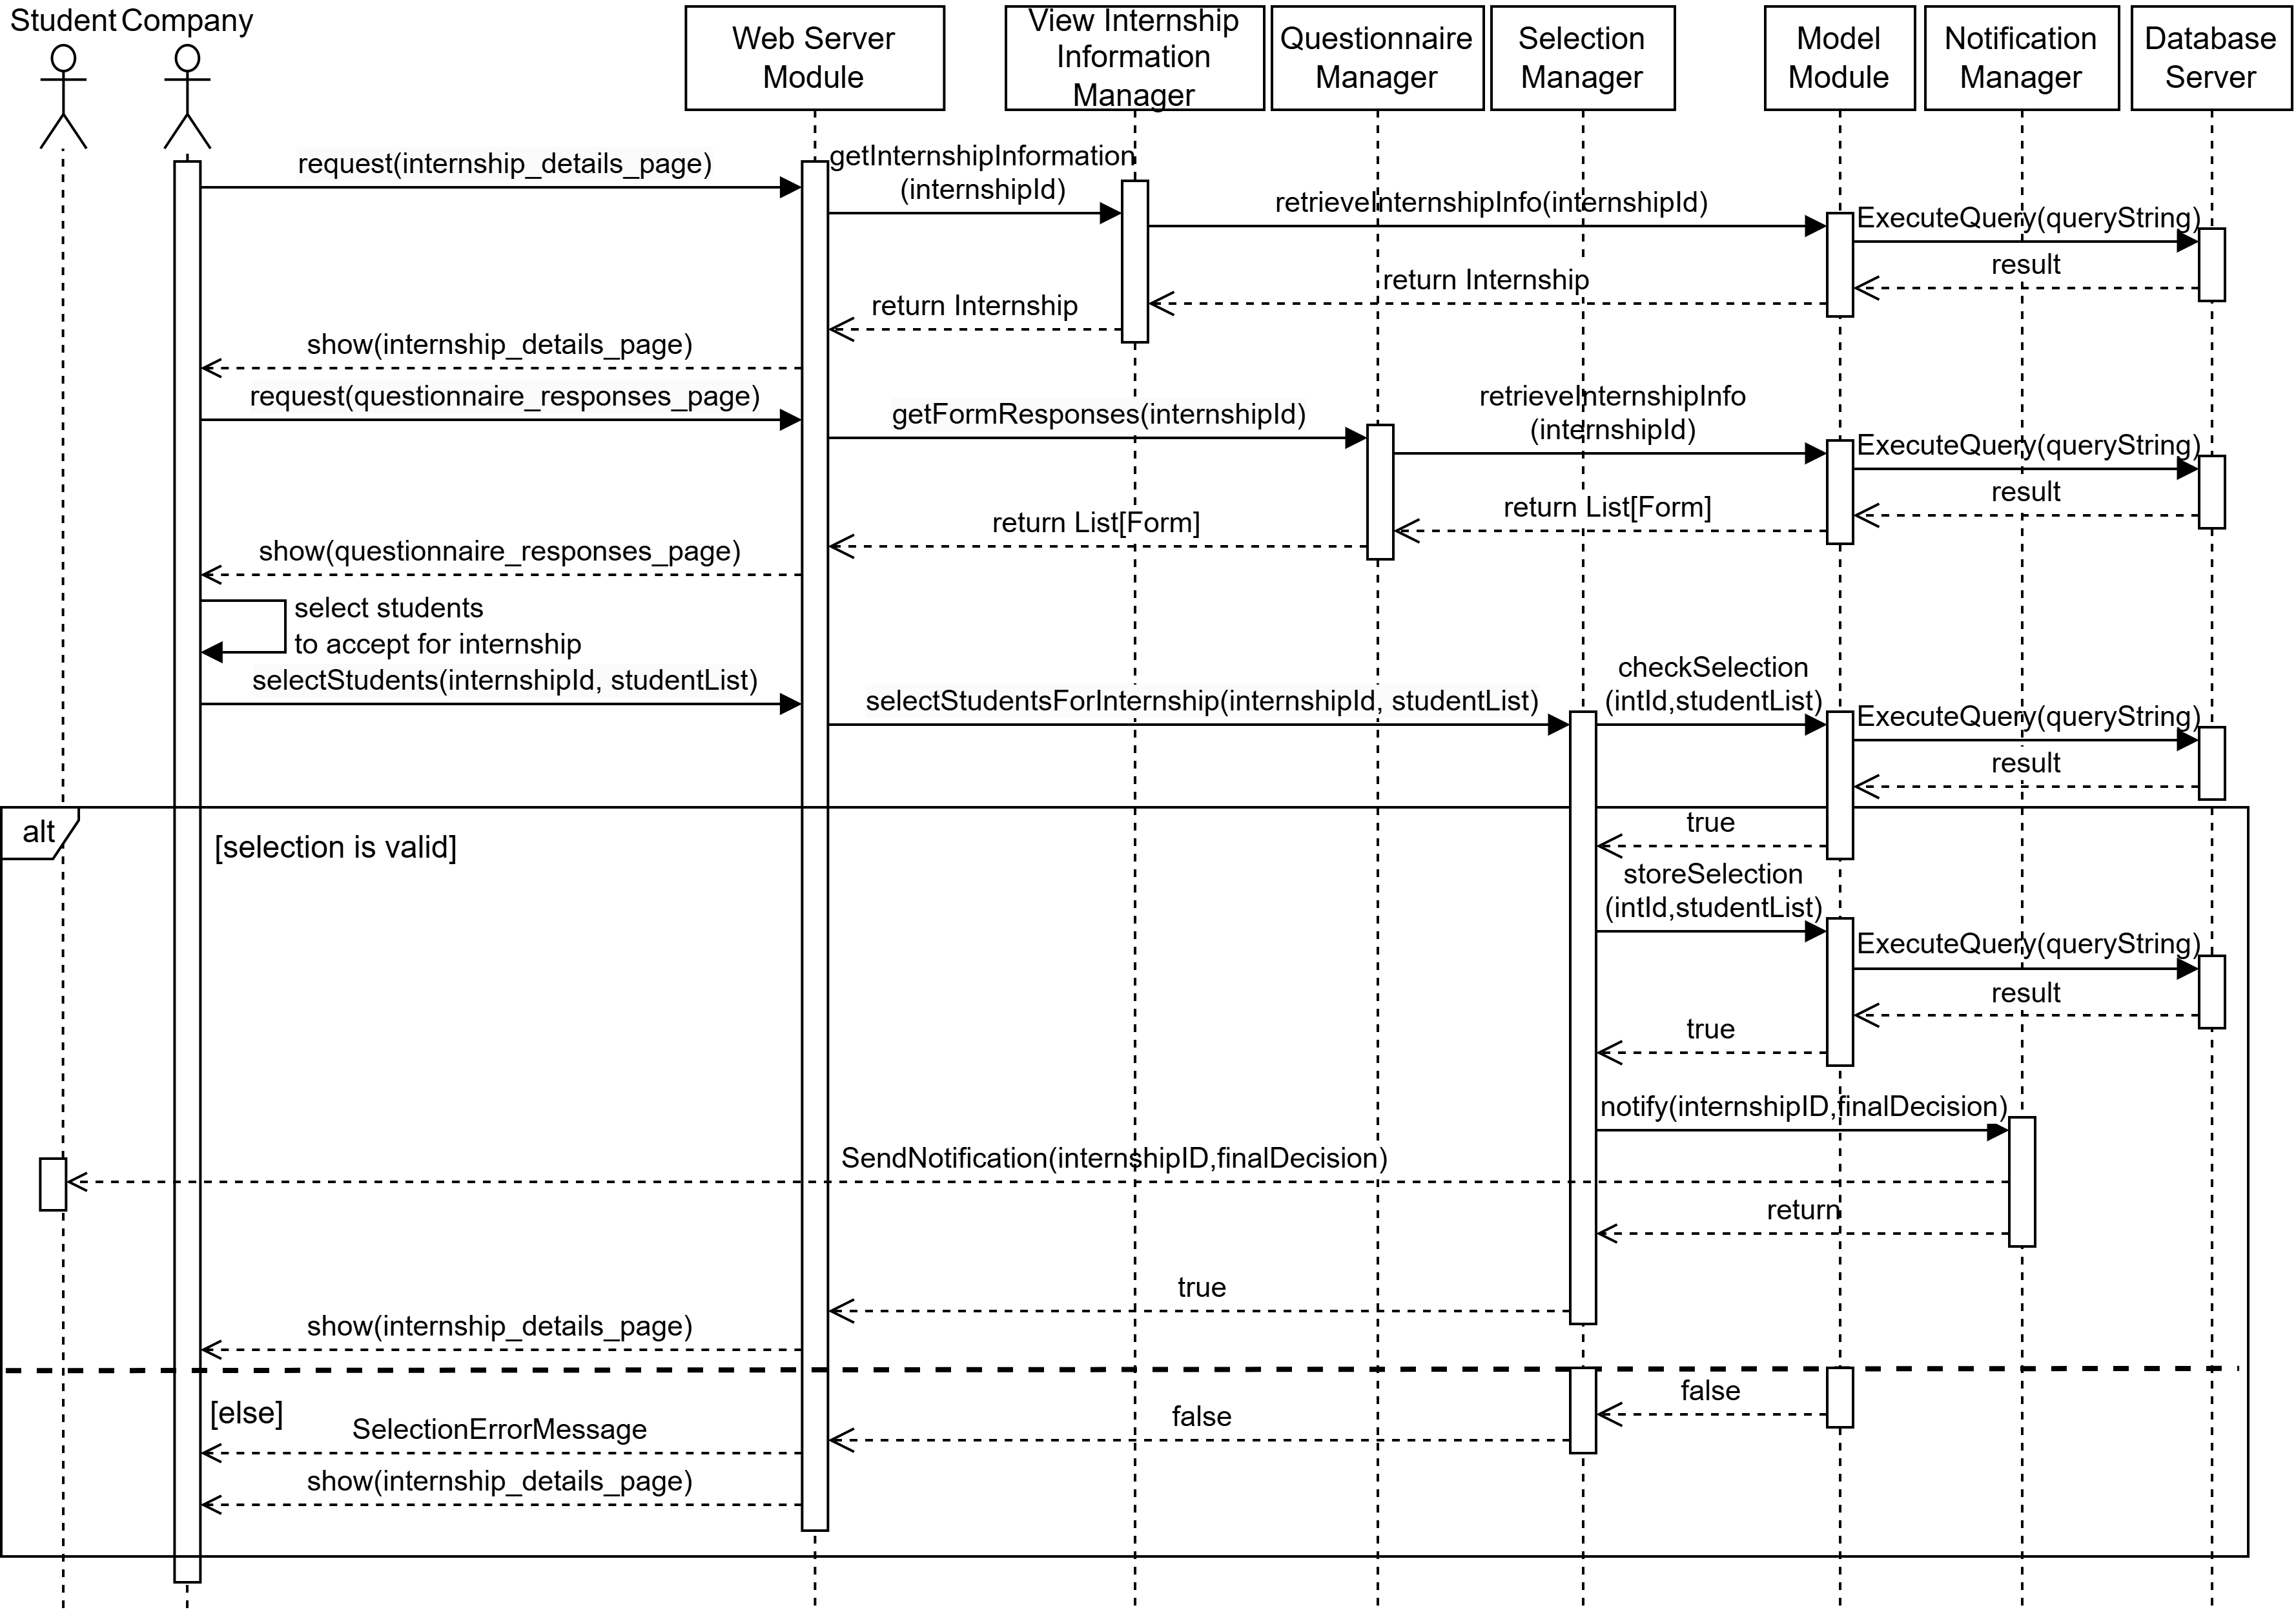
\includegraphics[width=1\textwidth]{Images/Runtime_view/intResults_SD.png}
    \caption{Company sends interview results Sequence Diagram}
\end{figure}
% Use Case 11
\begin{figure}[H]
    \centering
    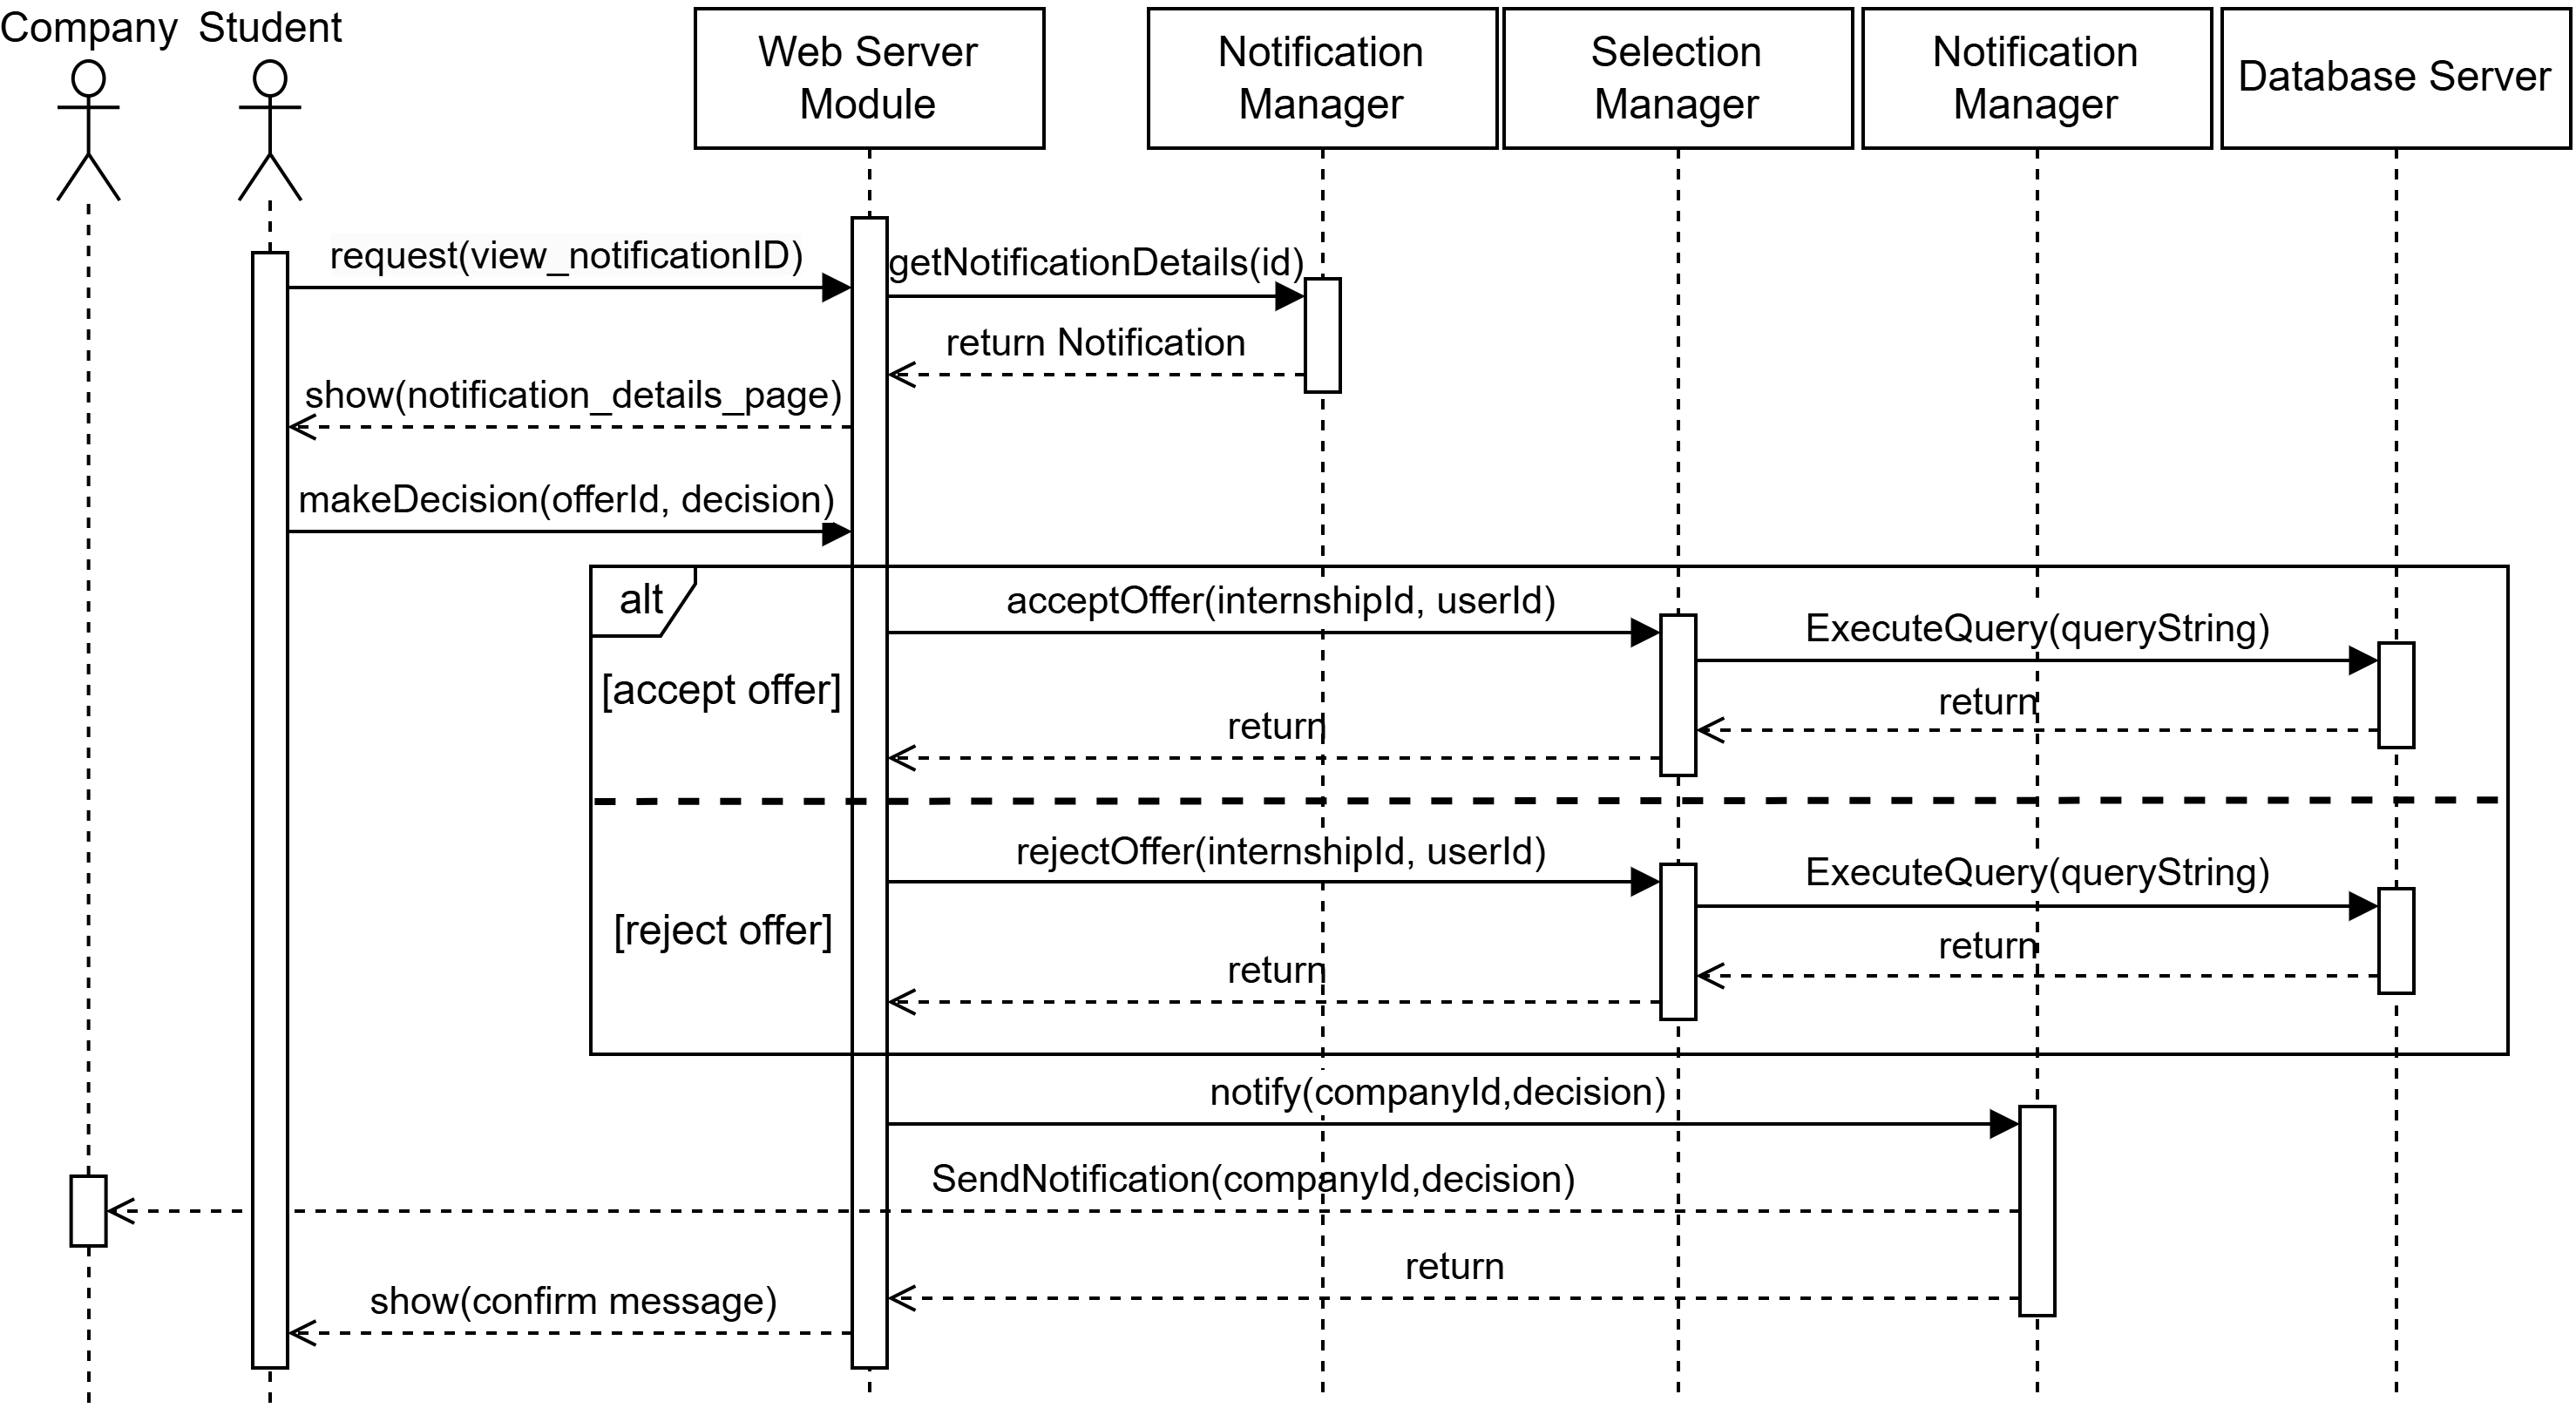
\includegraphics[width=1\textwidth]{Images/Runtime_view/acceptRej_SD.png}
    \caption{Student accepts/rejects an offer Sequence Diagram}
\end{figure}
% Use Case 12
\begin{figure}[H]
    \centering
    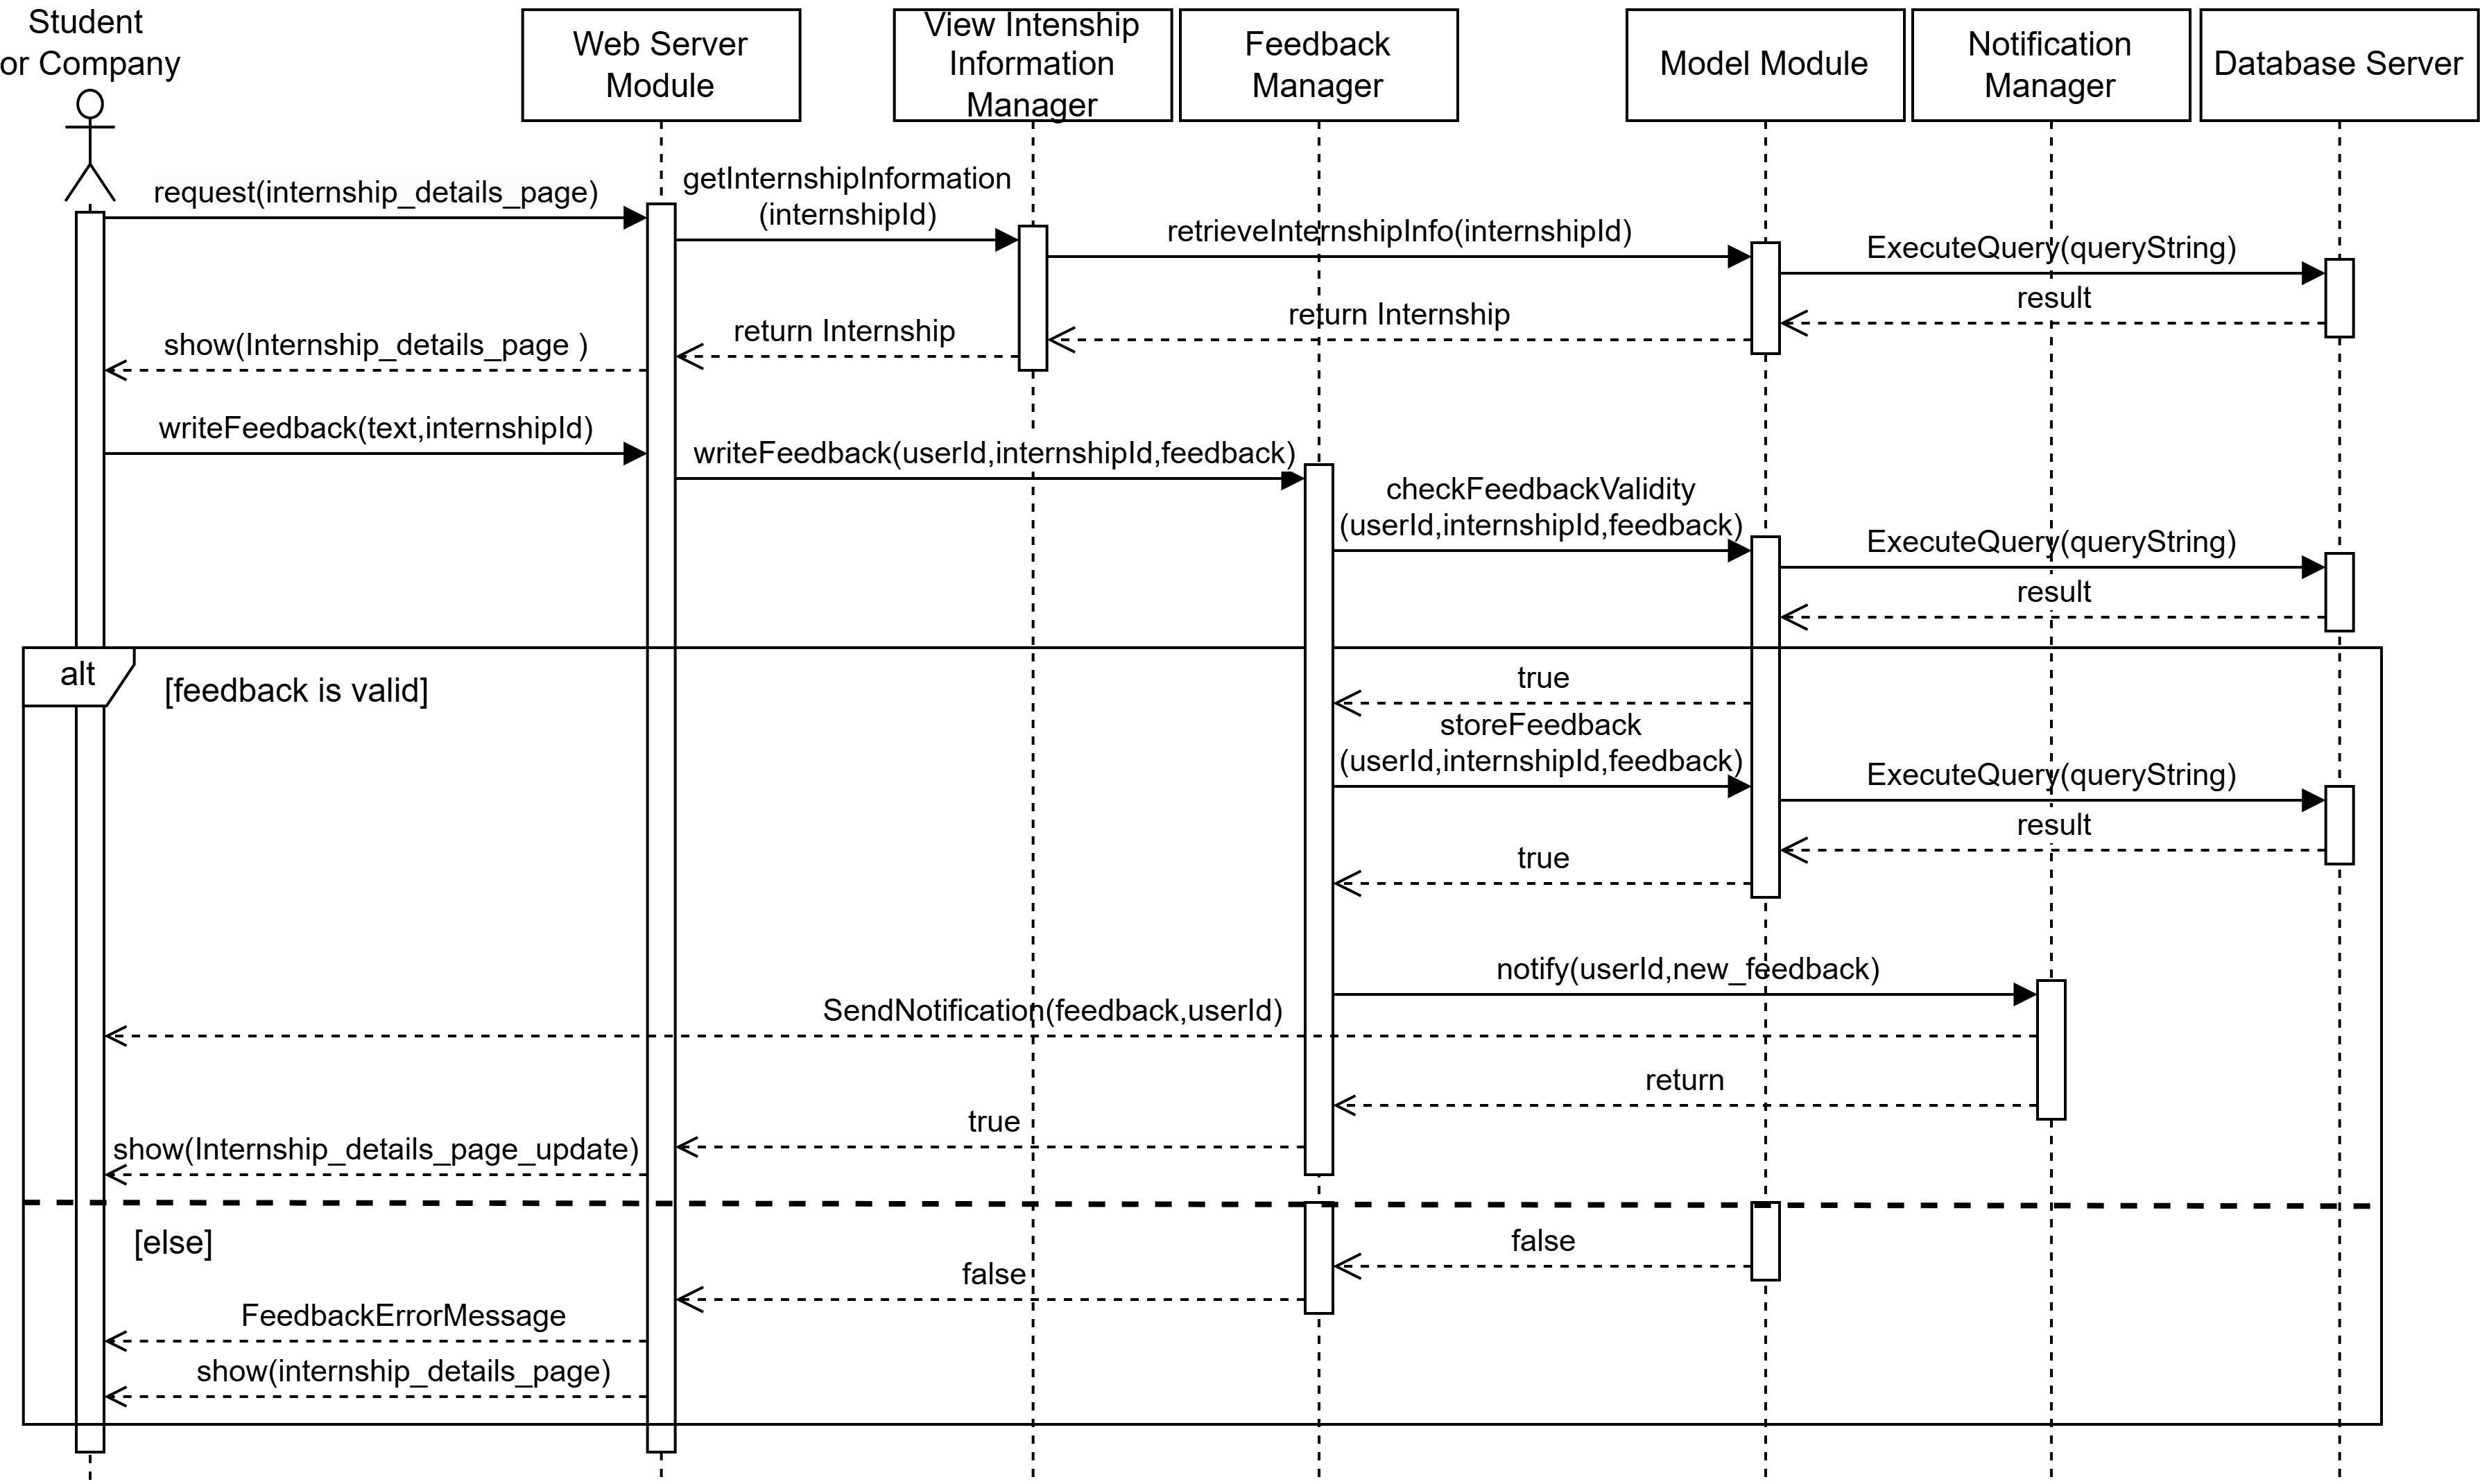
\includegraphics[width=1\textwidth]{Images/Runtime_view/feedback_SD.png}
    \caption{Student or Company writes feedback Sequence Diagram}
\end{figure}
% Use Case 13
\begin{figure}[H]
    \centering
    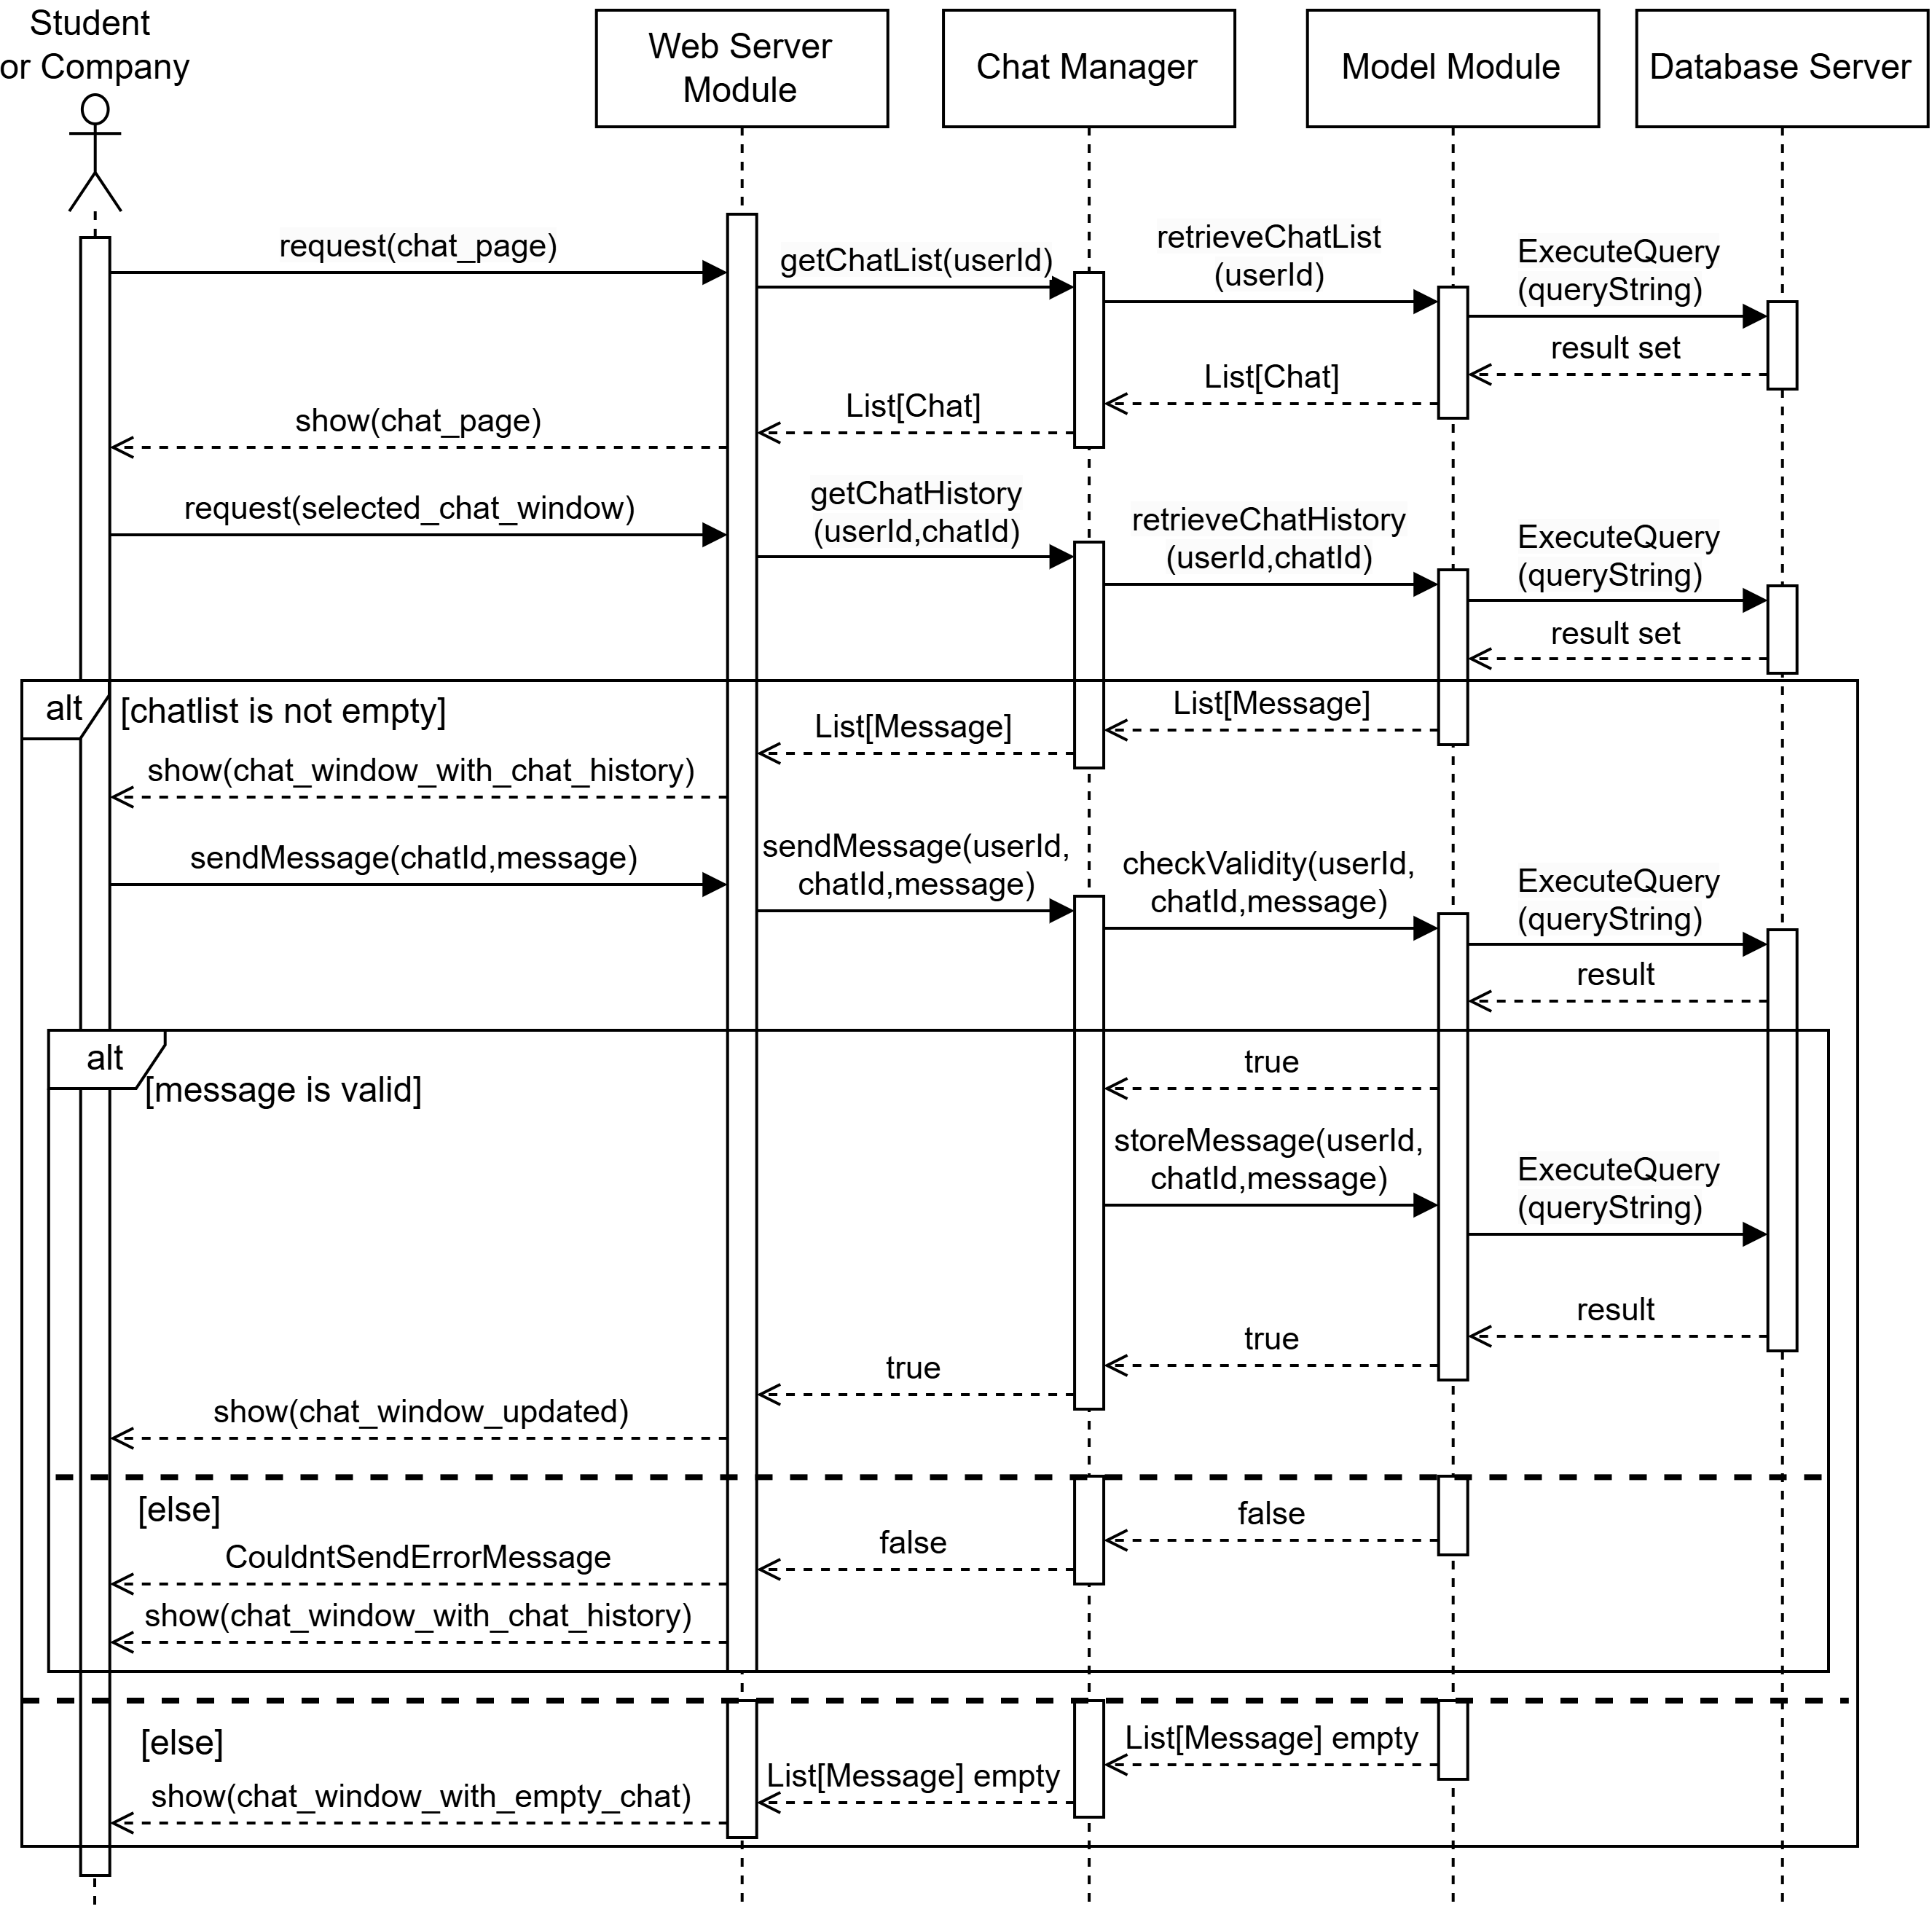
\includegraphics[width=0.86\textwidth]{Images/Runtime_view/chatting_SD.png}
    \caption{Student or Company chats with each other Sequence Diagram}
\end{figure}
% Use Case 14
\begin{figure}[H]
    \centering
    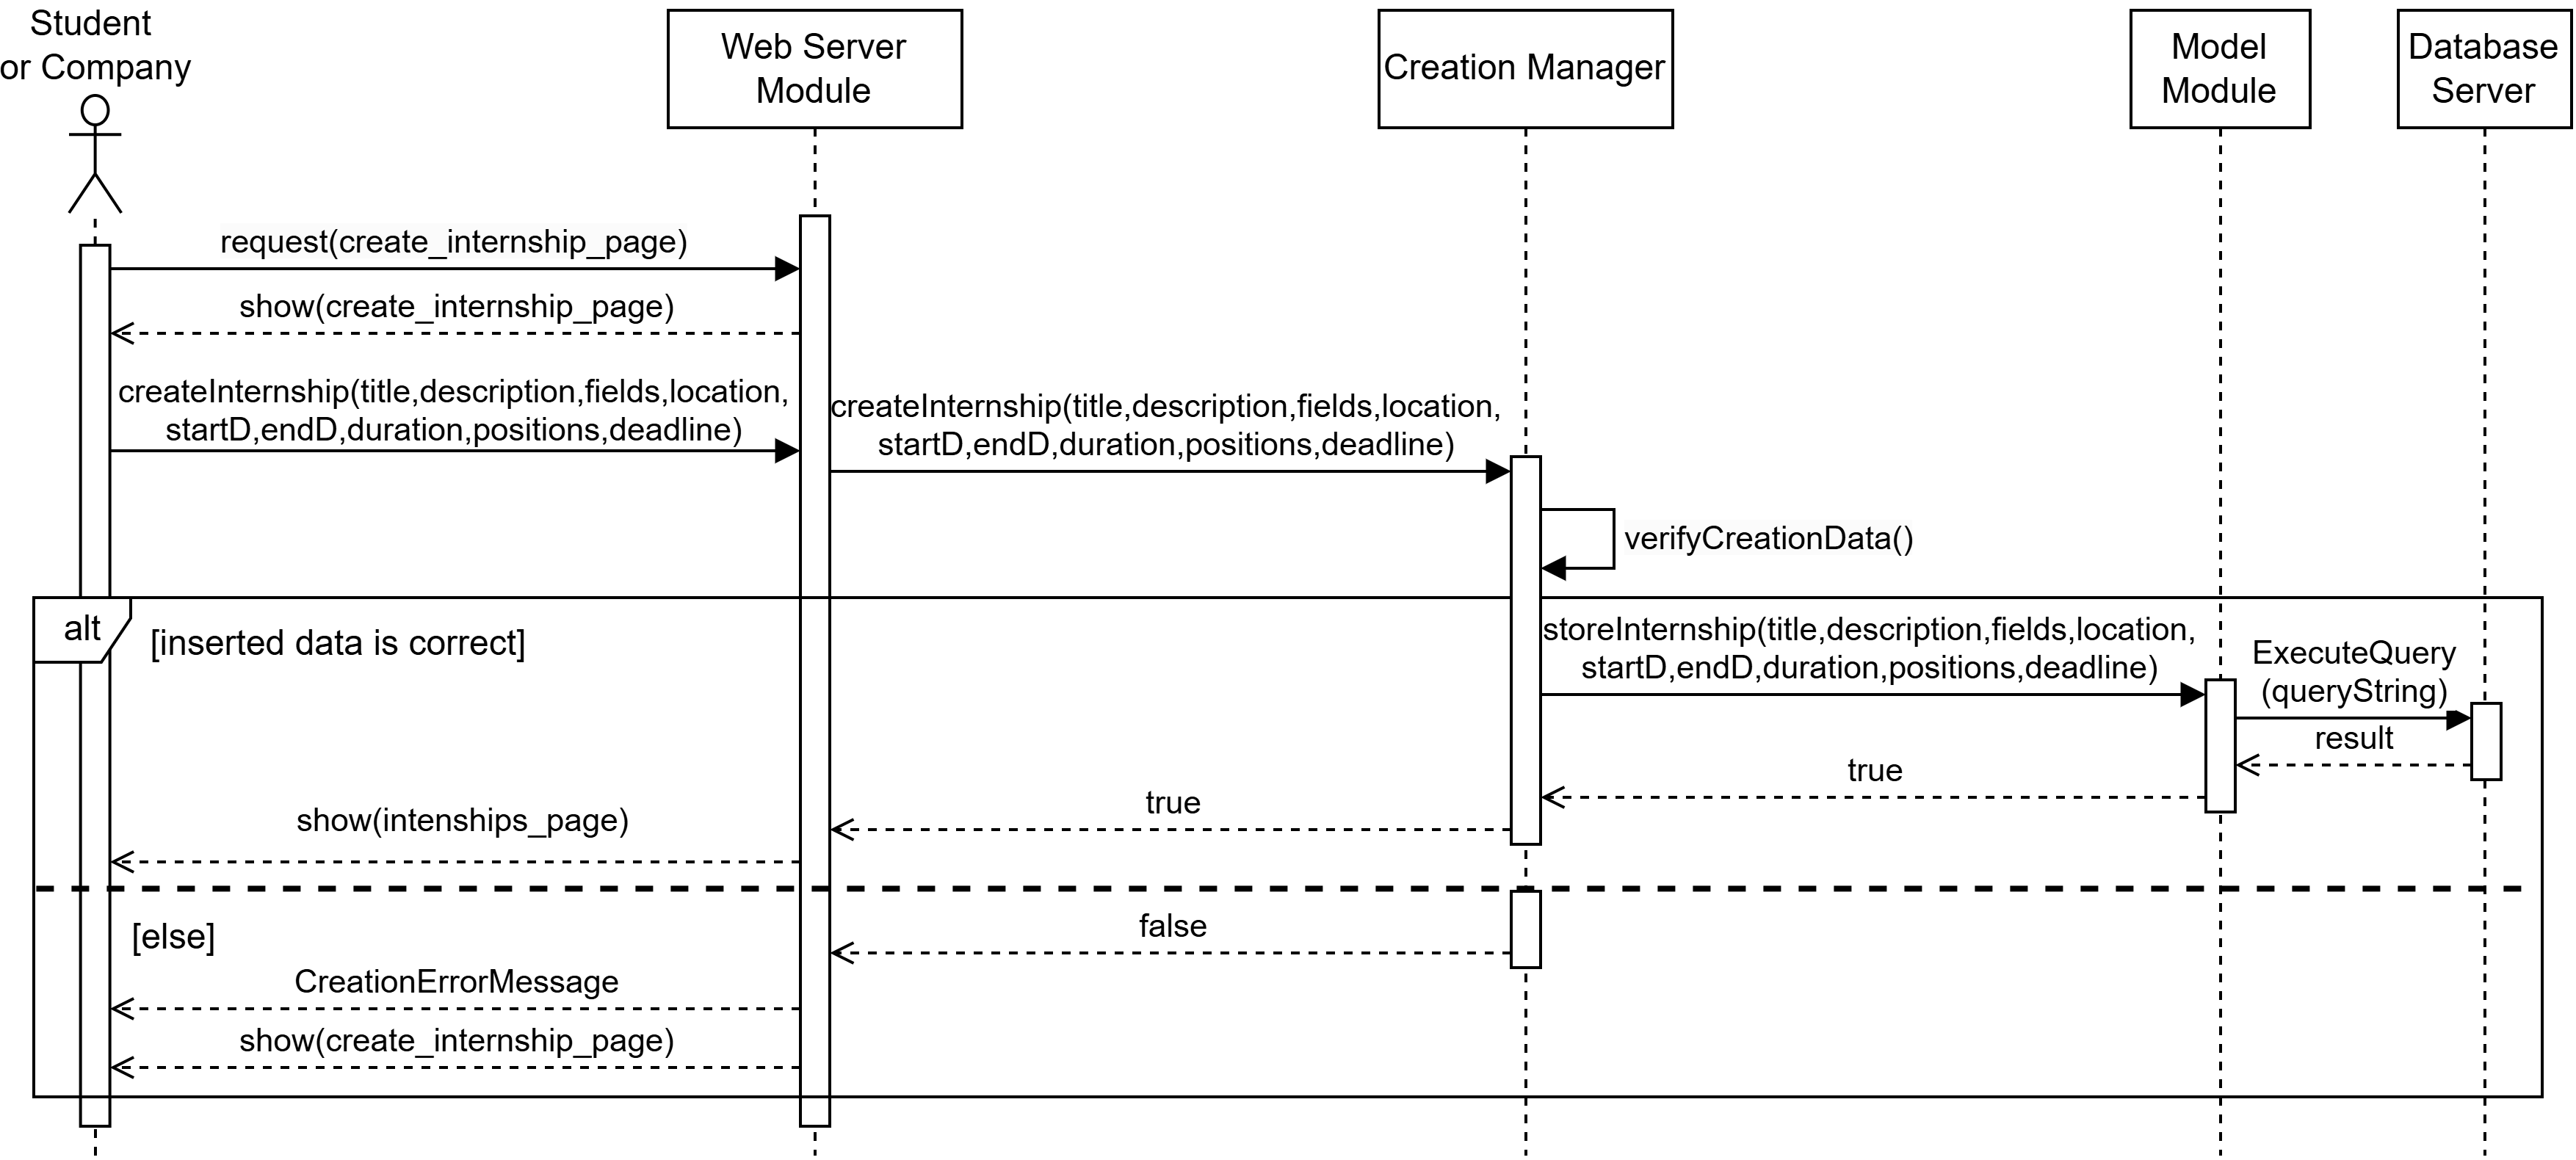
\includegraphics[width=0.94\textwidth]{Images/Runtime_view/createInt_SD.png}
    \caption{Company creates and publishes an internship Sequence Diagram}
\end{figure}
% Use Case 15
\begin{figure}[H]
    \centering
    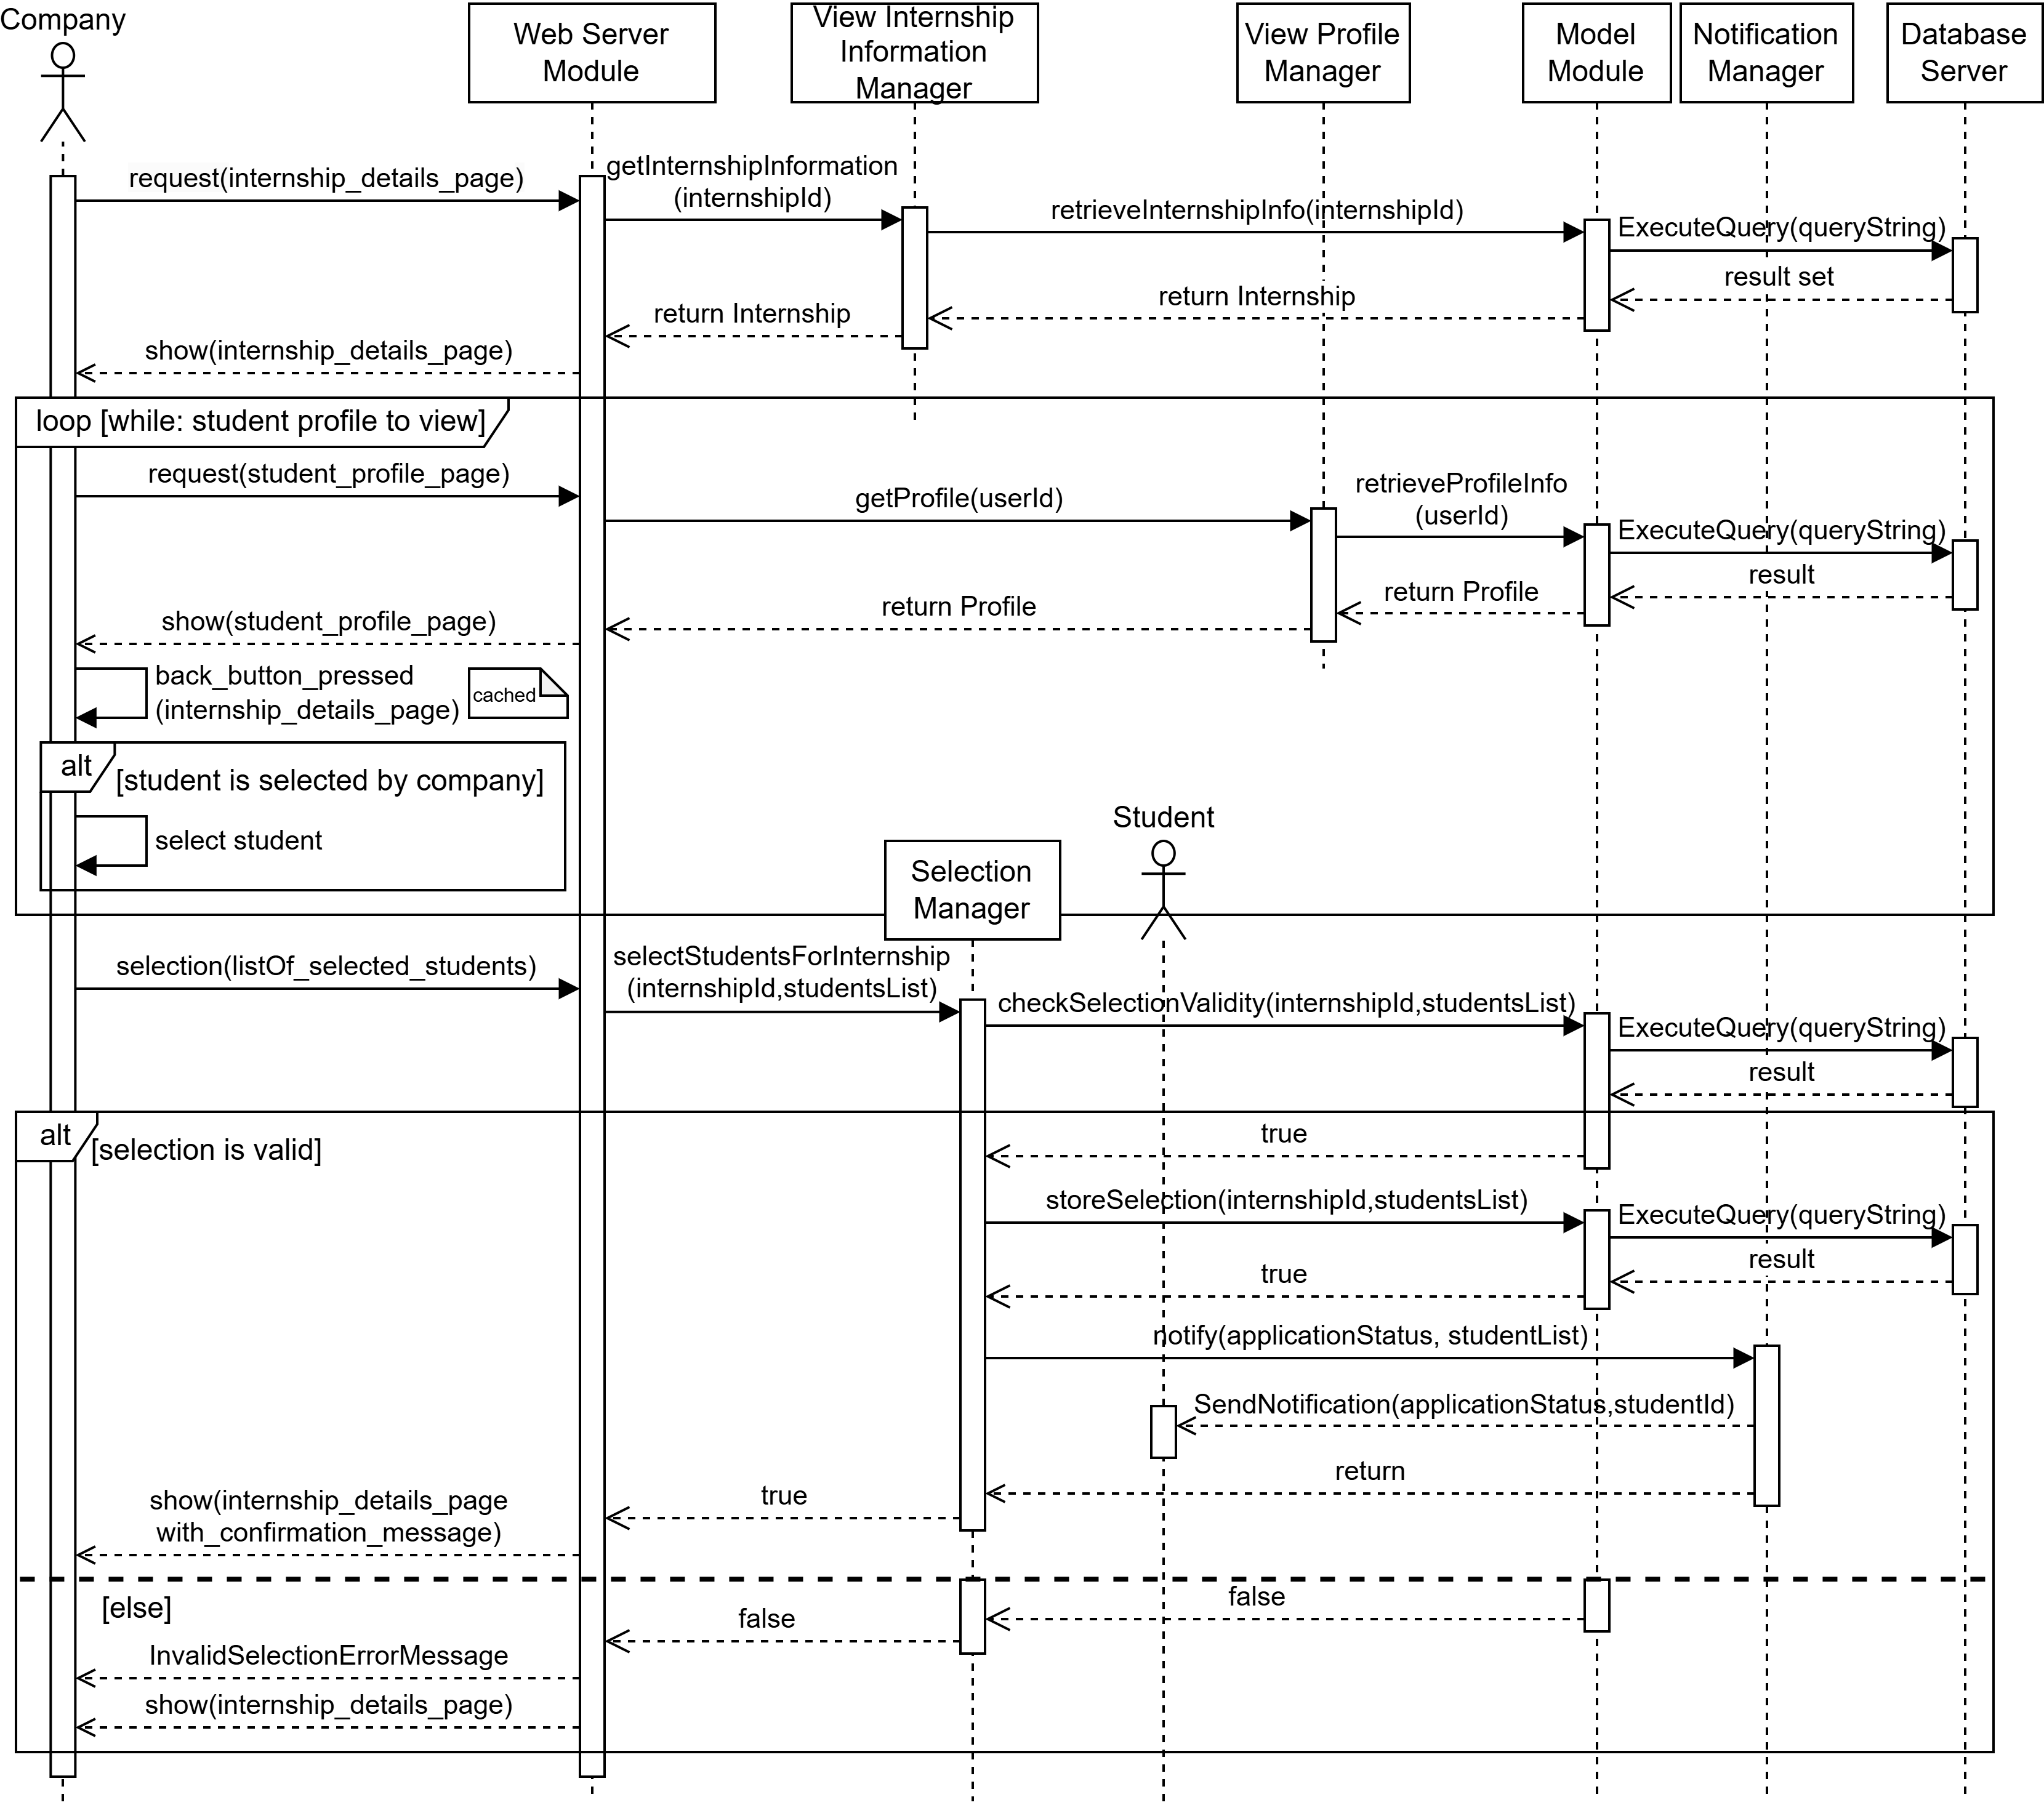
\includegraphics[width=1\textwidth]{Images/Runtime_view/select_SD.png}
    \caption{Company selects candidates Sequence Diagram}
\end{figure}
% Use Case 16
\begin{figure}[H]
    \centering
    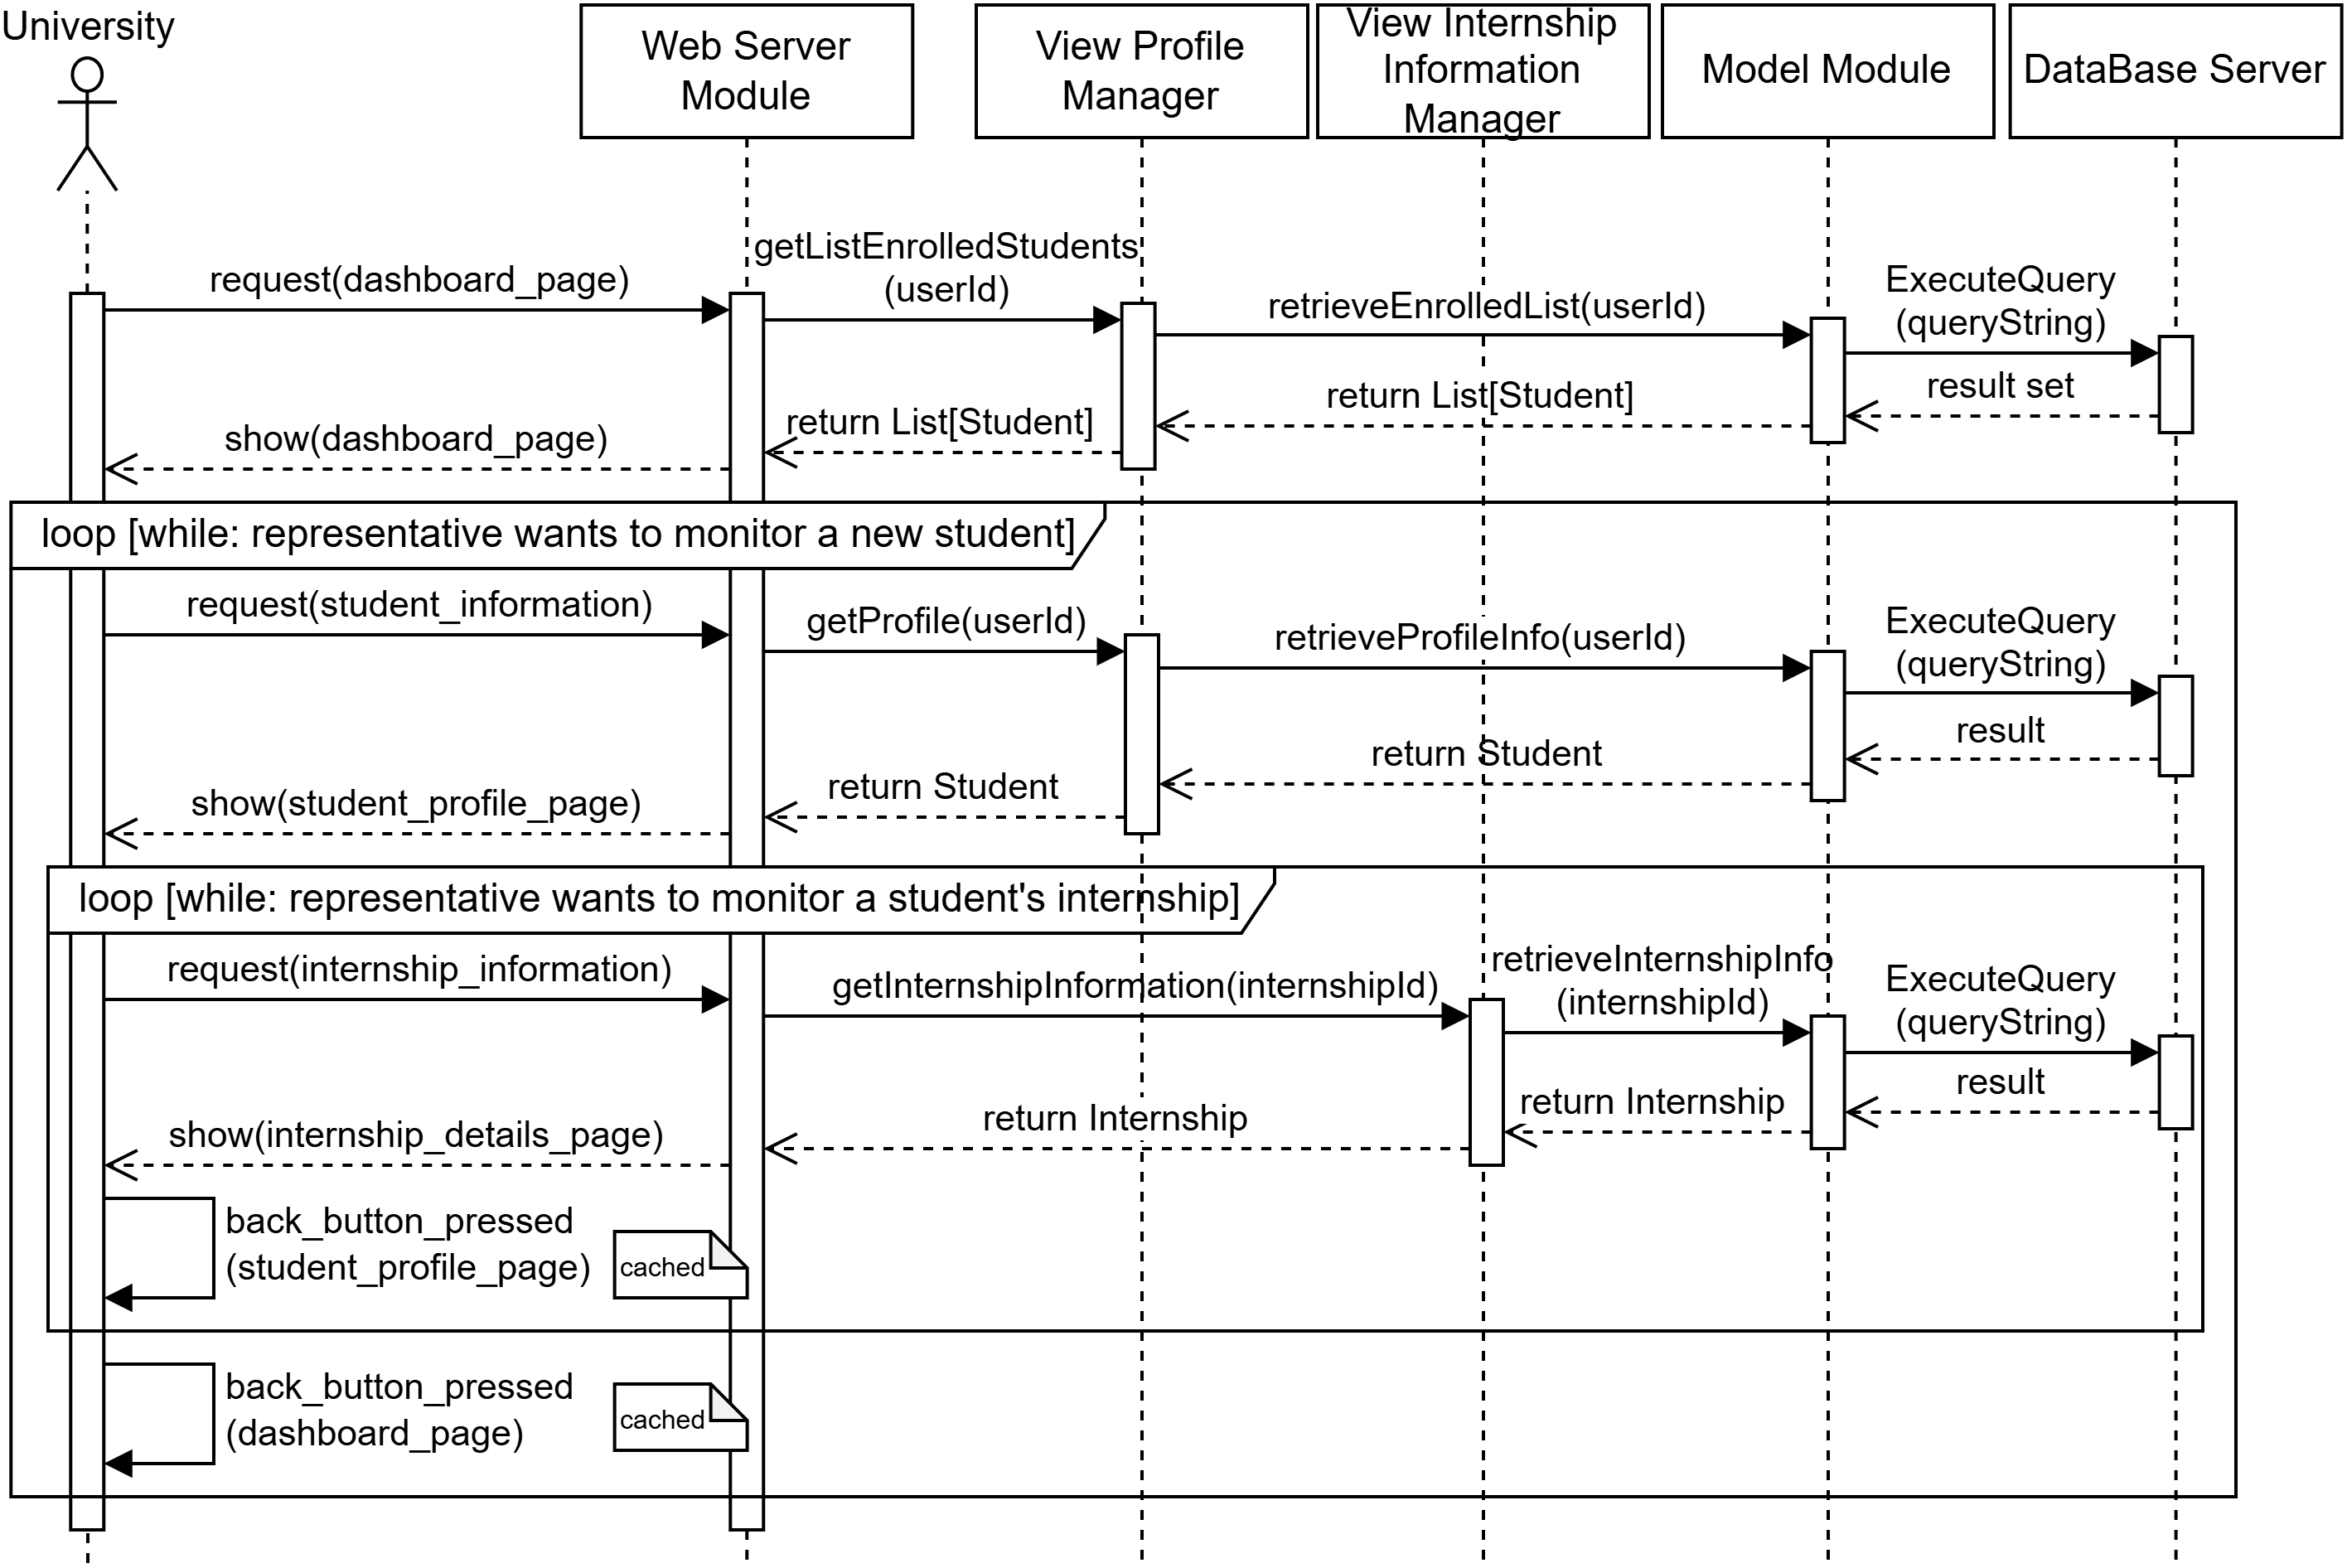
\includegraphics[width=1\textwidth]{Images/Runtime_view/monitor_SD.png}
    \caption{University monitors the internship processes of students Sequence Diagram}
\end{figure}


\section{Selected architectural styles and patterns}\label{sec:selected architectural styles and patterns}
\subsection{Three-Tiered Architecture}\label{subsec:three-tiered architecture}
As described in Section Overview, the Students\&Companies (S\&C) platform is build using a multi-tier architecture. This decision was made with the aim of 
providing a more scalable and flexible system.
The system is divided into three main layers: the presentation layer, the application layer, and the data layer.
Each layer has its own responsibilities and plays a specific role in the system: the presentation layer serves as the front end, accessible through the GUI, 
while the application layer and data layer together form the back end of the system, accessible via API-based methods.
\begin{itemize}
    \item \textbf{Presentation Layer:} The presentation layer is implemented as a generic web application accessible through a web browser.
    It is responsible for managing the presentation logic, including user interaction, the user interface, and rendering information.
    This layer serves as the front end of the system, the only part that the user can access directly.
    \item \textbf{Application Layer:} The application layer is implemented as a set of RESTful web services.
    It is responsible for managing the functional logic of the system, controlling communication between the presentation layer and the data layer.
    This layer allows the system to react to user input and generate appropriate responses accordingly.
    It includes the Application Server and is also used to interact with third-party services.
    \item \textbf{Data Layer:} The data layer is responsible for managing the data storage and access within the system.
    All operations that require data manipulation must be performed through interactions with the data layer.
    The platform uses a Relational Database Management System (RDBMS), making the data accessible through SQL queries.
\end{itemize}
\subsection{RESTful API}\label{subsec:restful api}
The Representational State Transfer (REST) style is designed to be stateless, enabling more efficient and seamless communication between the client and the 
server. It uses standard HTTP methods (GET, POST, PUT, DELETE) to perform operations on resources.
The decision to incorporate RESTful APIs into the architecture provides advantages in terms of performance, modifiability, and simplicity by defining conventions 
for interacting with resources in resource-oriented manner.
\subsection{Model-View-Controller (MVC) Pattern}\label{subsec:model-view-controller pattern}
One of the most recommended design patterns for the Three-Tier Architecture is the Model-View-Controller (MVC) pattern. It separates the application into three 
components: the model, the view, and the controller, minimizing interdependencies between the components and improving the maintainability, manageability, and 
scalability of the system. Each component can be developed, tested, and maintained independently.
\begin{itemize}
\item \textbf{Model:} Contains the state and application logic and is independent of the other components.
\item \textbf{View:} Represents the visual presentation logic of the Model and is responsible for displaying data to the user.
\item \textbf{Controller:} Acts as an intermediary between the Model and the View. It receives user input forwarded by the View, then processes operations and 
updates the Model and the View accordingly.
\end{itemize}

\section{Other design decisions}\label{sec:other design decisions}
\begin{itemize}
    \item \textbf{Design patterns related to the behavioral aspects:} Observer Pattern and State Pattern.
    \item \textbf{Design decisions related to the system's requirements:} Some design decisions are already described in the RASD, such as reliability, 
    availability, scalability, security, maintainability, and portability. 
    The following sections revisit availability, scalability, and security to emphasize their importance in the system.
\end{itemize}
\subsection{Observer Pattern}\label{subsec:observer pattern}
The Observer pattern is particularly useful when multiple objects need to be notified about a change in the state of another object. In the context of the 
S\&C platform, a large number of functionalities require the participation of multiple objects, such as notifying users about the results of an interview or 
updates on the status of an application.
\subsection{State Pattern}\label{subsec:state pattern}
The State pattern is recommended to efficiently manage operations across different states and handle transitions between them, as it allows objects to change 
their behavior when their internal state changes. In the context of the S\&C platform, the State pattern can be used to manage the lifecycle of an application 
for a internship position.

\subsection{Availability}\label{subsec:availability}
The system is designed to be highly available, ensuring that users can access the platform at any time, as described in the RASD, with at least 99.8 percent 
uptime. To achieve this, critical components should be replicated across multiple servers to provide redundancy and fault tolerance in case of failure. Load 
balancing is correctly configured to distribute incoming traffic, preventing overload on any single server. Continuous monitoring of the system's performance 
allows for the detection and resolution of any issues that may arise in real-time.
\subsection{Scalability}\label{subsec:scalability}
The platform is designed to handle increased user loads in the future by scaling individual layers independently, thanks to the architectural styles and patterns 
mentioned earlier. As described in the RASD, the system can be scaled horizontally by adding more servers or vertically by increasing the resources of existing 
servers, without affecting performance. This scalability is essential, especially as the number of users grows, leading to a higher volume of application 
requests over time.
\subsection{Security}\label{subsec:security}
The system is designed to ensure the privacy and security of user data both during transmission over the network and while stored in the database. This includes 
the use of authentication and authorization mechanisms to ensure that only authorized users can access the system, reducing the risk of unauthorized access. 
Additionally, a firewall and Intrusion Detection System (IDS) are set up in the network to protect the system from external threats and attacks. Protocols like 
HTTPS are used to encrypt communication between the client and server, and other encryption algorithms are employed to protect sensitive data stored in the 
database, such as user passwords.
